%%%%%%%%%%%%%%%%%%%%%%%%%%%%%%%%%
% Cerca la parola TODO all'interno di questo file per individuare ciò che devi personalizzare.
%%%%%%%%%%%%%%%%%%%%%%%%%%%%%%%%%
%
%
%


% Comandi per generare PDF-A2 con i relativi metadati 
\begin{filecontents*}[overwrite]{\jobname.xmpdata}
\Title{TODO Titolo del documento PDF}
\Author{TODO Nome autore}
\Language{it}
\Subject{TODO Breve frase descrittiva}
\Keywords{TODO\sep keyword2\sep keyword3}
\end{filecontents*}


%%%%%%%%%%%%%%%%%%%%%%%%%%%%%%%%%
%   PREAMBOLO DEL DOCUMENTO     %
%%%%%%%%%%%%%%%%%%%%%%%%%%%%%%%%%
\documentclass[a4paper,12pt,oneside,top=3cm,bottom=3cm,left=3.5cm,right=3.5cm,openright,reqno,table]{book}
% openany - fa iniziare i capitoli direttamente nella pagina successiva
% openright - fa iniziare i capitoli nella prima pagina destra disponibile 
% fleqn  - allinea le formule a sinistra anzichè centrarle
% leqno - dispone la numerazione delle formule sulla sinistra o destra
% reqno - dispone la numerazione delle formule sulla destra

% package fondamentali
\usepackage{graphicx}
\usepackage[T1]{fontenc}
\usepackage[utf8]{inputenc}
% se si realizza un documento in piu lingue bisogna istruire babel con
% [lingua_secondaria,lingua_principale]
\usepackage[italian]{babel}
\usepackage{colorprofiles}
\usepackage[colorlinks,hyperindex,pagebackref]{hyperref}
\hypersetup{
			citecolor=black,
			filecolor=black,
			linkcolor=black,
			urlcolor=black
}
% per generare il PDF-A2
\usepackage[a-2b,mathxmp]{pdfx}[2018/12/22]
\hypersetup{pdfstartview=}

% tutti i package sono specificati in un file a parte: packages.sty
\usepackage{packages}

% comandi personalizzati
\usepackage{utils}

% stile dei capitoli
\usepackage[SeSa]{fncychap}

% gli stili di capitolo disponibili sono i seguenti:
% SeSa, Sonny, Lenny, Rejne, Conny, PetersLenny, Bjornstrup, Glenn, Bjarne, Nicola

\linespread{1.5}

%%%%%%%%%%%%%%%%%%%%%%%%%%%%%%%%%
%   DOCUMENTO VERO E PROPRIO    %
%%%%%%%%%%%%%%%%%%%%%%%%%%%%%%%%%
\begin{document}

% frontespizio 
\begin{titlepage}
\changepage{}{}{}{-7.5 mm}{}{}{}{}{}
% parametri per cambiare le dimensioni di una singola pagina in ordine:
% {textheight}{textwidth}{evensidemargin}{oddsidemargin}{columnsep}
% {topmargin}{headheight}{headsep}{footskip}
% se voglio centrare la pagina devo mettere bindingoffset/2
% i primi 5 parametri posso usarli con \changetext


\begin{center}
\vspace{0.5cm}

\includegraphics [width=.15\columnwidth, angle=0]{covermatter/figure/logo-unisa}\\ % height
{\Large \scshape Università degli Studi di Salerno}\\
\vspace{0.5cm}
{\Large Dipartimento di Informatica}\\
\vspace{0.5cm}
{\Large Corso di Laurea Triennale in Informatica}\\
\vspace{1.5cm}
{\Large \scshape Tesi di Laurea} \\
\vspace{4cm}
{\Huge \bfseries Titolo della Tesi} \\
\vspace{4cm}

\begin{minipage}[t]{7cm}
\flushleft
{\large \textsc{Relatore}}

{\large Prof. Nome relatore} \\
{\large Dott. Nome tutor} \\
Università degli Studi di Salerno \\[0.25cm]
\end{minipage}
\hfill
\begin{minipage}[t]{7cm}
\flushright
{\large \textsc{Candidato}}

{\large \textbf{Nome Cognome}} \\
Matricola: 0123456789
\end{minipage}

\vspace{3cm}

{\small Anno Accademico YYYY-YYYY} %\\
%
%
\end{center}

\end{titlepage}


% sesalab
\begin{titlepage}
\nonumber
\null \vspace {\stretch{1}}
\begin{flushright}
{\textit{Questa tesi è stata realizzata nel} \hspace*{0.25cm}}
\\
\vspace{0.5cm}

\includegraphics[width=.40\columnwidth, angle=0]{logo-sesa}
\end{flushright}
\end{titlepage}


%dedica
\begin{titlepage}
\nonumber
\null \vspace {\stretch{1}}
	\begin{flushright}
%	\begin{verse}
\textit{Sono interessato al futuro perché vi passerò il resto della mia vita.} \\[5mm]

    Charles Franklin Kettering
%	\end{verse}
	\end{flushright}
\end{titlepage}

% abstract
\renewcommand{\abstractname}{Abstract}
\label{Abstract}

\begin{center}

\Large
\textbf{Abstract}
    
\end{center}


La presente tesi si propone di esplorare e implementare soluzioni avanzate di gestione dei dati per migliorare l'efficienza e l'efficacia del reparto di assistenza tecnica di un'azienda. La ricerca è suddivisa in due fasi cruciali.

Nella prima fase, vengono analizzati approfonditamente i concetti chiave relativi ai Big Data, data warehousing, analisi dati e business intelligence. Questa fase di studio fornisce una base teorica solida per comprendere le sfide e le opportunità nel contesto aziendale.

La seconda fase si concentra sull'applicazione pratica dei concetti appresi durante lo studio iniziale. Dopo un dettagliato briefing con gli stakeholder aziendali, viene progettato e implementato un sistema di data warehousing e business intelligence personalizzato per il reparto di assistenza tecnica. L'obiettivo principale è quello di fornire agli operatori del reparto strumenti avanzati per analizzare dati in tempo reale, identificare tendenze e inefficienze, e prendere decisioni informate per ottimizzare i processi.

Il lavoro si propone di dimostrare come l'integrazione di tecnologie di data warehousing e business intelligence possa portare a miglioramenti significativi nelle operazioni quotidiane del reparto di assistenza tecnica, consentendo all'azienda di rispondere in modo più rapido ed efficace alle esigenze dei clienti. La tesi contribuisce quindi al progresso della gestione aziendale attraverso l'applicazione concreta di metodologie avanzate di analisi dati e business intelligence.

\frontmatter
% quello che segue è in numerazione romana e i capitoli non verranno numerati
% se non si vuole che compaia il numero di pagina basta usare il comando:
%\nonumber

% indici 
\phantomsection

% Il simbolo * serve per evitare che comapaia nell'indice

\tableofcontents
\clearpage

\addcontentsline{toc}{chapter}{Elenco delle Figure}
\listoffigures
\clearpage

\addcontentsline{toc}{chapter}{Elenco delle Tabelle}
\listoftables
\clearpage



\mainmatter
% quello che segue sarà in numerazione araba e i capitoli verranno numerati

% TODO inserire capitoli
\chapter{Introduzione}
\label{ch:Introduzione}

\begin{citazione}
Non esiste alternativa alla trasformazione digitale. Le aziende visionarie si ritaglieranno nuove opzioni strategiche, quelle che non si adatteranno falliranno. Jeff Bezos \cite{jeff_bezos_cite}
\end{citazione}

Ormai da anni il mondo ha inglobato nel proprio essere la tecnologia, rendendola parte di esso e in alcuni casi anche imprescindibile. L’evoluzione della tecnologia ha contribuito esponenzialmente alla produzione di nuovi sistemi che migliorassero la vita delle persone, con automazioni e semplificazioni dei normali compiti tediosi o stancanti. Tale evoluzione ha comportato una sempre più importante evoluzione delle infrastrutture atte a permettere la creazione di tali sistemi e soprattutto di un ambiente interconnesso. Proprio per questo motivo, al giorno d'oggi molto spesso si da per scontato la tecnologia e la sua interazione con il mondo. Tuttavia, ciò non va sottovalutato, l'avvento della tecnologia fin dal primo istante ha comportato l'evoluzione del mondo intero dovuto alla necessità di adattamento a quest'ultima. Con il tempo ogni persona ha fatto parte di questo processo, utilizzando tale innovazione e migliorando il proprio stile di vita. Naturalmente, tale evoluzione ha condizionato anche il mondo aziendale, prendendo il nome di \textbf{trasformazione digitale}; più precisamente questa pratica corrisponde al processo di evoluzione dei modelli aziendali, basato sugli avanzamenti tecnologici. Consiste in un cambiamento radicale attuato mediante strumenti digitali \cite{redhat_digital_transformation}.

\section{Trasformazione Digitale}
Lo sviluppo economico deriva molto spesso da diversi cambiamenti sociali avvenuti nel tempo. La \textit{trasformazione digitale} (o \textit{digital tranformation, DT}) è uno degli esempi più importanti e recenti che manifestano tale cambiamento. Proprio per questo motivo, molti ricercatori hanno studiato approfonditamente questo fenomeno in modo da poterne identificare le possibili implicazioni, vantaggi, svantaggi e conseguenze sulle pratiche sociali e lavorative. Tutto allo scopo di sfruttare al massimo tale processo in modo da farlo diventare un importante punto fondamentale che permetta di migliorare ulteriormente \cite{sciencedirect_digital_transformation}.

Secondo uno studio svolto nel 2018 è stato previsto che durante lo stesso anno sarebbero stati investiti circa 1,3 miliardi di dollari da parte delle aziende per applicare tecniche digitali in modo da incrementare l'efficienza, aumentare il valore del cliente e creare nuove opportunità di monetizzazione. Tuttavia, tale trasformazione non è affatto un compito semplice; infatti, il 70\% di questi processi non è riuscita o riuscirà nel proprio intento, comportando  una perdita totale di oltre 900 milioni di dollari \cite{forbes_digital_transformation_fail}.

\subsection{Strategie della Trasformazione Digitale}

A seguito di approfonditi studi e dell'incremento dell'interesse in questo mondo, molte aziende negli ultimi anni hanno intrapreso un processo di esplorazione e innovazione adoperando nuove tecnologie digitali così da poterne sfruttare i benefici. Ciò ha comportato la necessità di svolgere procedimenti atti a trasformare anche le principali operazioni svolte dalle aziende in questione. Però, per svolgere tale procedura è necessario formulare una strategia di trasformazione corretta e coordinata \cite{digital_transformation_strategies}.

\subsection{Benefici}

La maggior parte dei benefici della trasformazione digitale nell'ambito professionale possono essere suddivisi in cinque differenti gruppi ~\cite{sciencedirect_digital_transformation_benefits}:
\begin{itemize}
    \item Miglioramento della produttività: i processi di sviluppo e progettazione hanno diminuito le relative tempistiche necessarie per essere eseguiti.
    \item Incremento della qualità: tramite apposite misurazioni ad alta precisione dei parametri di produzione e dei prodotti durante l'interno processo di produzione è possibile comprendere al meglio tutte le sue fasi, così da conoscere su quale di questi svolgere delle azioni che comportino un risparmio.
    \item Maggiore personalizzazione dei prodotti: svolgendo analisi sui dati rispetto alle interazioni con gli utenti e ulteriori analisi di mercato è possibile comprendere quale siano le preferenze del proprio pubblico.
    \item Aumento della sicurezza: naturalmente l’evoluzione digitale porta non solo migliorie in ambito economico, ma anche in quello della sicurezza del singolo utente che, grazie a nuovi strumenti e metodologie, può svolgere in maggiore sicurezza (o magari non farlo proprio) compiti pericolosi, venendo preventivamente avvisato di potenziali rischi e sulle possibili contromisure.
\end{itemize}

\section{Incremento dei dati}

Sicuramente, tra i vari processi di trasformazione digitale, il principale è stato quello di dematerializzazione dei documenti cartacei, che prende il nome di \textbf{digitalizzazione} (o \textit{digitalization}). Più precisamente quando si parla di digitalizzazione si parla del processo di trasformazione di un'immagine, di un suono, di un documento in un formato digitale, interpretabile da un computer \cite{wikipedia_digitalization_definition}.

A seguito di tale processo, le informazioni nel formato digitale, che in precedenza non era stato nemmeno immaginato, hanno acquisito sempre più importanza nel mondo con il nome di \textit{dati} fino a diventare uno, se non il valore più importante.

Lo scopo di tale progetto era riorganizzare la conoscenza in modo sempre più efficiente, semplificando la selezione delle notizie in un mondo sommerso dalle informazioni. Fu compreso fin dal primo istante quanto questo fosse ambizioso, tuttavia, forse in parte venne sottostimato quale potesse essere la portata di tale rivoluzione. Tale idea ha determinato non solo la ridistribuzione e organizzazione delle informazioni pregresse, ma anche la creazione di nuove informazioni dovute proprio a tale processo di modernizzazione. A queste, si sono poi aggiunte sempre più dati da dover salvare e gestire, dovute all'aumento del numero di nuove tecnologie messe a disposizione dal progresso evolutivo che il mondo stava e sta tutt'ora affrontando. 

\subsection{La Digital DataSphere}

L'azienda IDC \footnote{La \textit{International Data Corporation} (\textit{IDC}) è un fornitore globale di informazioni di mercato, servizi di consulenza ed eventi per i mercati della tecnologia dell'informazione, delle telecomunicazioni e della tecnologia di consumo.} ha localizzato e definito i tre principali ambienti dove la digitalizzazione avviene di continuo e dove tali dati vengono salvati, ovvero \cite{idc_digital_datasphere}:

\begin{enumerate}
    \item \textit{Core} (o “nucleo”): consiste nei datacenter tradizionali e cloud messi a disposizione dai provider;
    \item \textit{Edge} (o “bordo”): ovvero le infrastrutture delle imprese/aziende che non fanno parte dei datacenter principali; 
    \item \textit{Endpoint} (o “estremo”): sono tutti i dispositivi personali che posizionati agli estremi della rete, come PC, smartphone, dispositivi IoT, eccetera. 
\end{enumerate}
Per una maggiore comprensione, è stata di seguito riportata nella figura \ref{fig:Digital-Datasphere} una raffigurazione visiva di tale schema.

\begin{figure}[H]
    \centering
    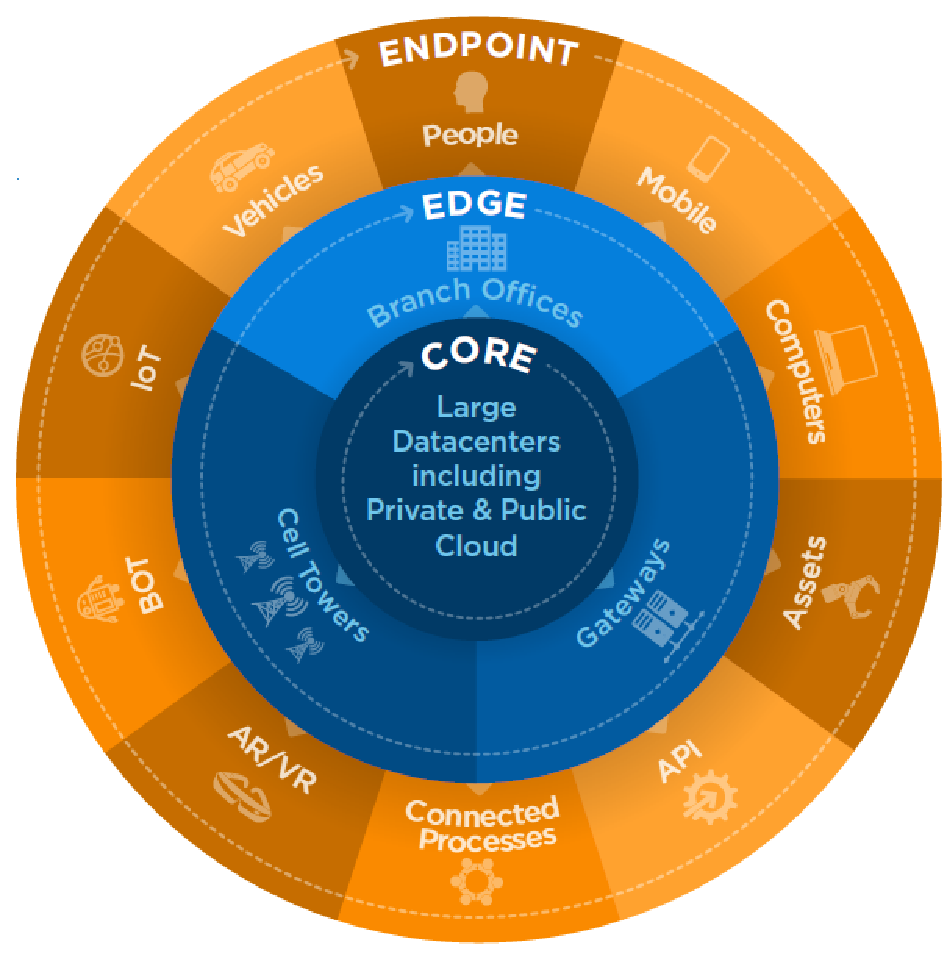
\includegraphics[width=0.5\linewidth]{figure/capitolo_1/Digital-Datasphere.pdf}
    \caption{Digital DataSphere}
    \label{fig:Digital-Datasphere}
\end{figure}

La somma di tutti questi dati forma ciò che loro definiscono come \textbf{Global DataSphere}; più precisamente la Global DataSphere quantifica ed analizza l'ammontare dei dati creati, recuperati e duplicati in un dato anno nell'intero mondo \cite{datadrivendaily_dimension_table}.

Secondo uno studio del 2018 svolto sull'incremento di tale Global DataSphere \cite{idc_global_datasphere}, la IDC ha denotato un andamento al quanto impressionante di tipo esponenziale. Ovvero secondo le stime entro il 2025 l'ammontare dei dati generati nell'intero mondo sarà pari a 175 Zettabyte (\textit{ZB}, ovvero 270 bit) rispetto ai "soli" 80 del 2022. Leggendo il grafico riportato nella figura \ref{fig:Annual Size Global Datasphere}, è possibile notare che nel triennio 2023-2025 è stata stimato l'ammontare di 430 Zettabyte di dati, mentre andando dal 2022 a ritroso l'ammontare totale è minore di 400; in altre parole, i dati dell'ultimo triennio superano il totale dei dati creati fino al 2022 dall'inizio della storia della digitalizzazione. Per poter comprendere meglio e farsi un'idea di quanto questo valore sia elevato, riporto qui un esempio: se volessimo scaricare l'intero DataSphere del 2025, ovvero 175 ZB di dati, con una connessione di 100 Mb/s \footnote{Il valore preso in esempio è stato ricavato facendo riferimento alla media italiana di velocità di download, verificata nel 2022 \cite{github_speed_connection}, e poi approssimato per semplicità di calcolo.} sarebbero necessari 554.552.923 anni (o più "semplicemente" 554.553 millenni) per completare l'operazione.

\begin{figure}[!h]
    \centering
    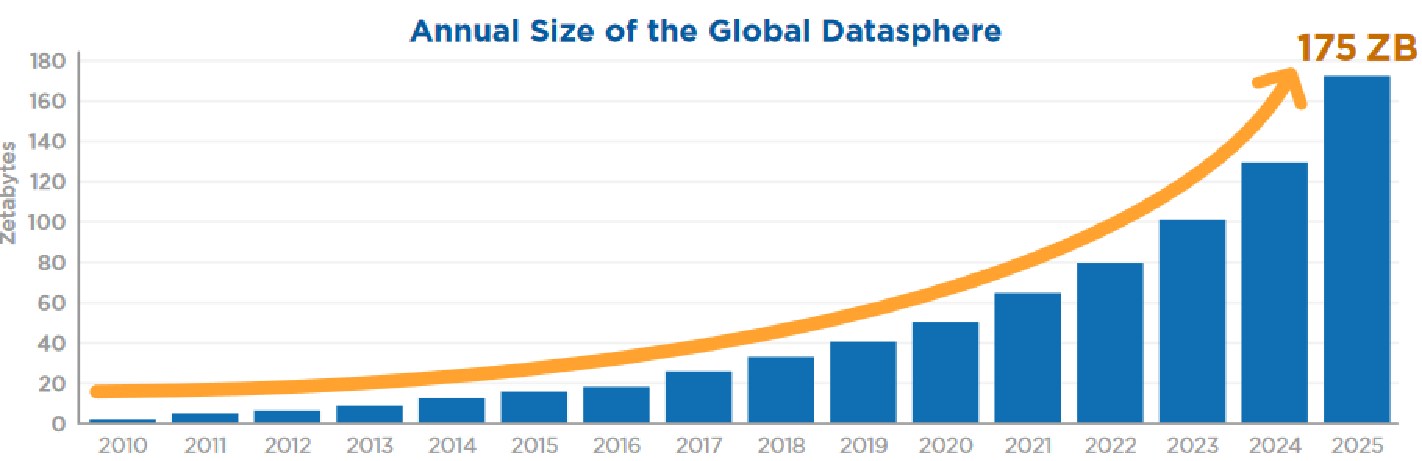
\includegraphics[width=1\linewidth]{figure/capitolo_1/Annual Size Global Datasphere.pdf}
    \caption{Dimensione annuale della Digital Datasphere globale}
    \label{fig:Annual Size Global Datasphere}
\end{figure}

\subsection{Salvataggio e Gestione Dati}

Naturalmente, come è possibile dedurre autonomamente, questo incremento della generazione dei dati è dovuto a molteplici fattori. Su tutti, sicuramente l'aumento di dispositivi utilizzabili per la generazione di tali dati e l'espansione nel mondo dell'Internet e del Web con tutti i relativi servizi annessi sono le maggiori cause. Attualmente siamo in un'era dove l'immensa quantità di dispositivi a nostra disposizione danno la possibilità alle persone di eseguire un'enorme quantità di azioni e interazioni, che non fanno altro che generare ulteriori dati e informazioni. L'incremento di tali dati ha generato in questo modo anche la necessità di salvarli e gestirli. Per questo motivo, lo storage dei dati, ovvero la raccolta e la conservazione di informazioni digitali, svolge un ruolo sempre più centrale nella gestione dei dati \cite{redhat_data_storage}.

Più precisamente quando si parla di \textit{gestione dei dati} si riferisce al processo di acquisizione, archiviazione e utilizzo dei dati che consente di sapere quali dati sono disponibili, dove si trovano, chi ne è il proprietario, chi può vederli e chi vi può accedere. Perciò, la gestione dei dati consente alle organizzazioni di eseguire il deployment delle applicazioni e dei sistemi critici in modo sicuro e conveniente e di facilitare le decisioni strategiche \cite{redhat_data_management}.

\section{Data-Driven Orientation}

Un aspetto molto importante, ma che purtroppo viene molto sottovalutato all'interno delle aziende, è la conoscenza reale del dato ancora prima della sua fruizione. Questo poiché non è possibile estrapolare informazioni da dati che si hanno a disposizione se non si ha una idea chiara su cosa essi possano effettivamente indicare e valorizzare. Proprio per sopperire a tale problematica, ormai l'approccio \textit{data-driven}, o \textit{data oriented}, è diventato sempre più comune nella maggior parte delle aziende.

\subsection{Il Processo Decisionale Basato Sui Dati}

La strategia di effettuare delle decisioni basate sui dati è stata introdotta per far risaltare l'importanza di questo nuovo orientamento che considera la raccolta dei dati come un punto cardine delle strategie aziendali. L'adozione di un insieme integrato di tecnologie apposite per l'analisi dei dati può contribuire a facilitare la comunicazione in tempo reale, coinvolgere gli attori nella presa di decisioni e consentire la costante ridefinizione delle interazioni tra gli utenti e la tecnologia così da migliorare il benessere ed ottenere, con l'avanzare del tempo, innovazione e resilienza \cite{emerald_data_driven_orientation}.

Più precisamente, il \textit{processo decisionale basato sui dati} (\textit{data-driven decision making, DDDM}) si definisce come l'utilizzo di elementi concreti, metriche e dati per orientare il processo decisionale aziendale in linea con obiettivi, scopi e iniziative. Cambiare il modo in cui la tua azienda prende decisioni non è semplice, ma incorporare dati e analisi nei cicli decisionali è il modo più efficace per l'evoluzione dell'organizzazione. Proprio per questo motivo, per una compagnia è necessario rendere il processo decisionale data-driven una prassi \cite{tableau_data_driven_decision_making}.

\subsection{Punti Chiave Delle Aziende Data-Driven}
Le aziende data-driven basano la loro organizzazione su cinque punti chiave \cite{researchgate_data_driven_orientation}:

\begin{enumerate}
    \item \textit{Digital transformation}. Per poter integrare i dati all'interno dei processi decisionali è necessario che questi siano presenti e disponibili. Per permettere ciò è necessaria una chiara strategia di trasformazione digitale.
    \item \textit{Data Science}. Con l'adozione di strumenti tecnologici, il modo in cui le organizzazioni producono, condividono e sfruttano i dati è cambiato radicalmente. Per tale motivo la Data Science (ovvero, lo studio dei dati per estrarre informazioni significative per il business) ha trovato nuovi modi per analizzare e ottenere valore dai dati.
    \item \textit{Data-Driven Business Model}. Al fine di generare ulteriore valore economico, le intuizioni aziendali acquisite devono essere sfruttate all'interno dei modelli di business. Una parte cruciale di questo processo è proprio la creazione di valore dalle informazioni digitalizzate, definendo come un DDBM si basi principalmente sul vedere i dati come una risorsa economicamente importante su cui investire.
    \item \textit{Data-Driven innovation}. Le aziende utilizzano i dati, da loro generati e raccolti, per trasformare le loro attività commerciali in innovazioni basate su questi. Attraverso tale innovazione, le organizzazioni sono adibite ad utilizzare e gestire coerentemente le loro enormi quantità di dati.
    \item \textit{Data Analytics}. Il valore dei dati ricercato deriva da un'attenta, corretta e congruente analisi dei dati a disposizione. Tale analisi permette alle compagnie di incrementare al meglio le proprie conoscenze aziendali.
\end{enumerate}

\begin{figure}[H]
    \centering
    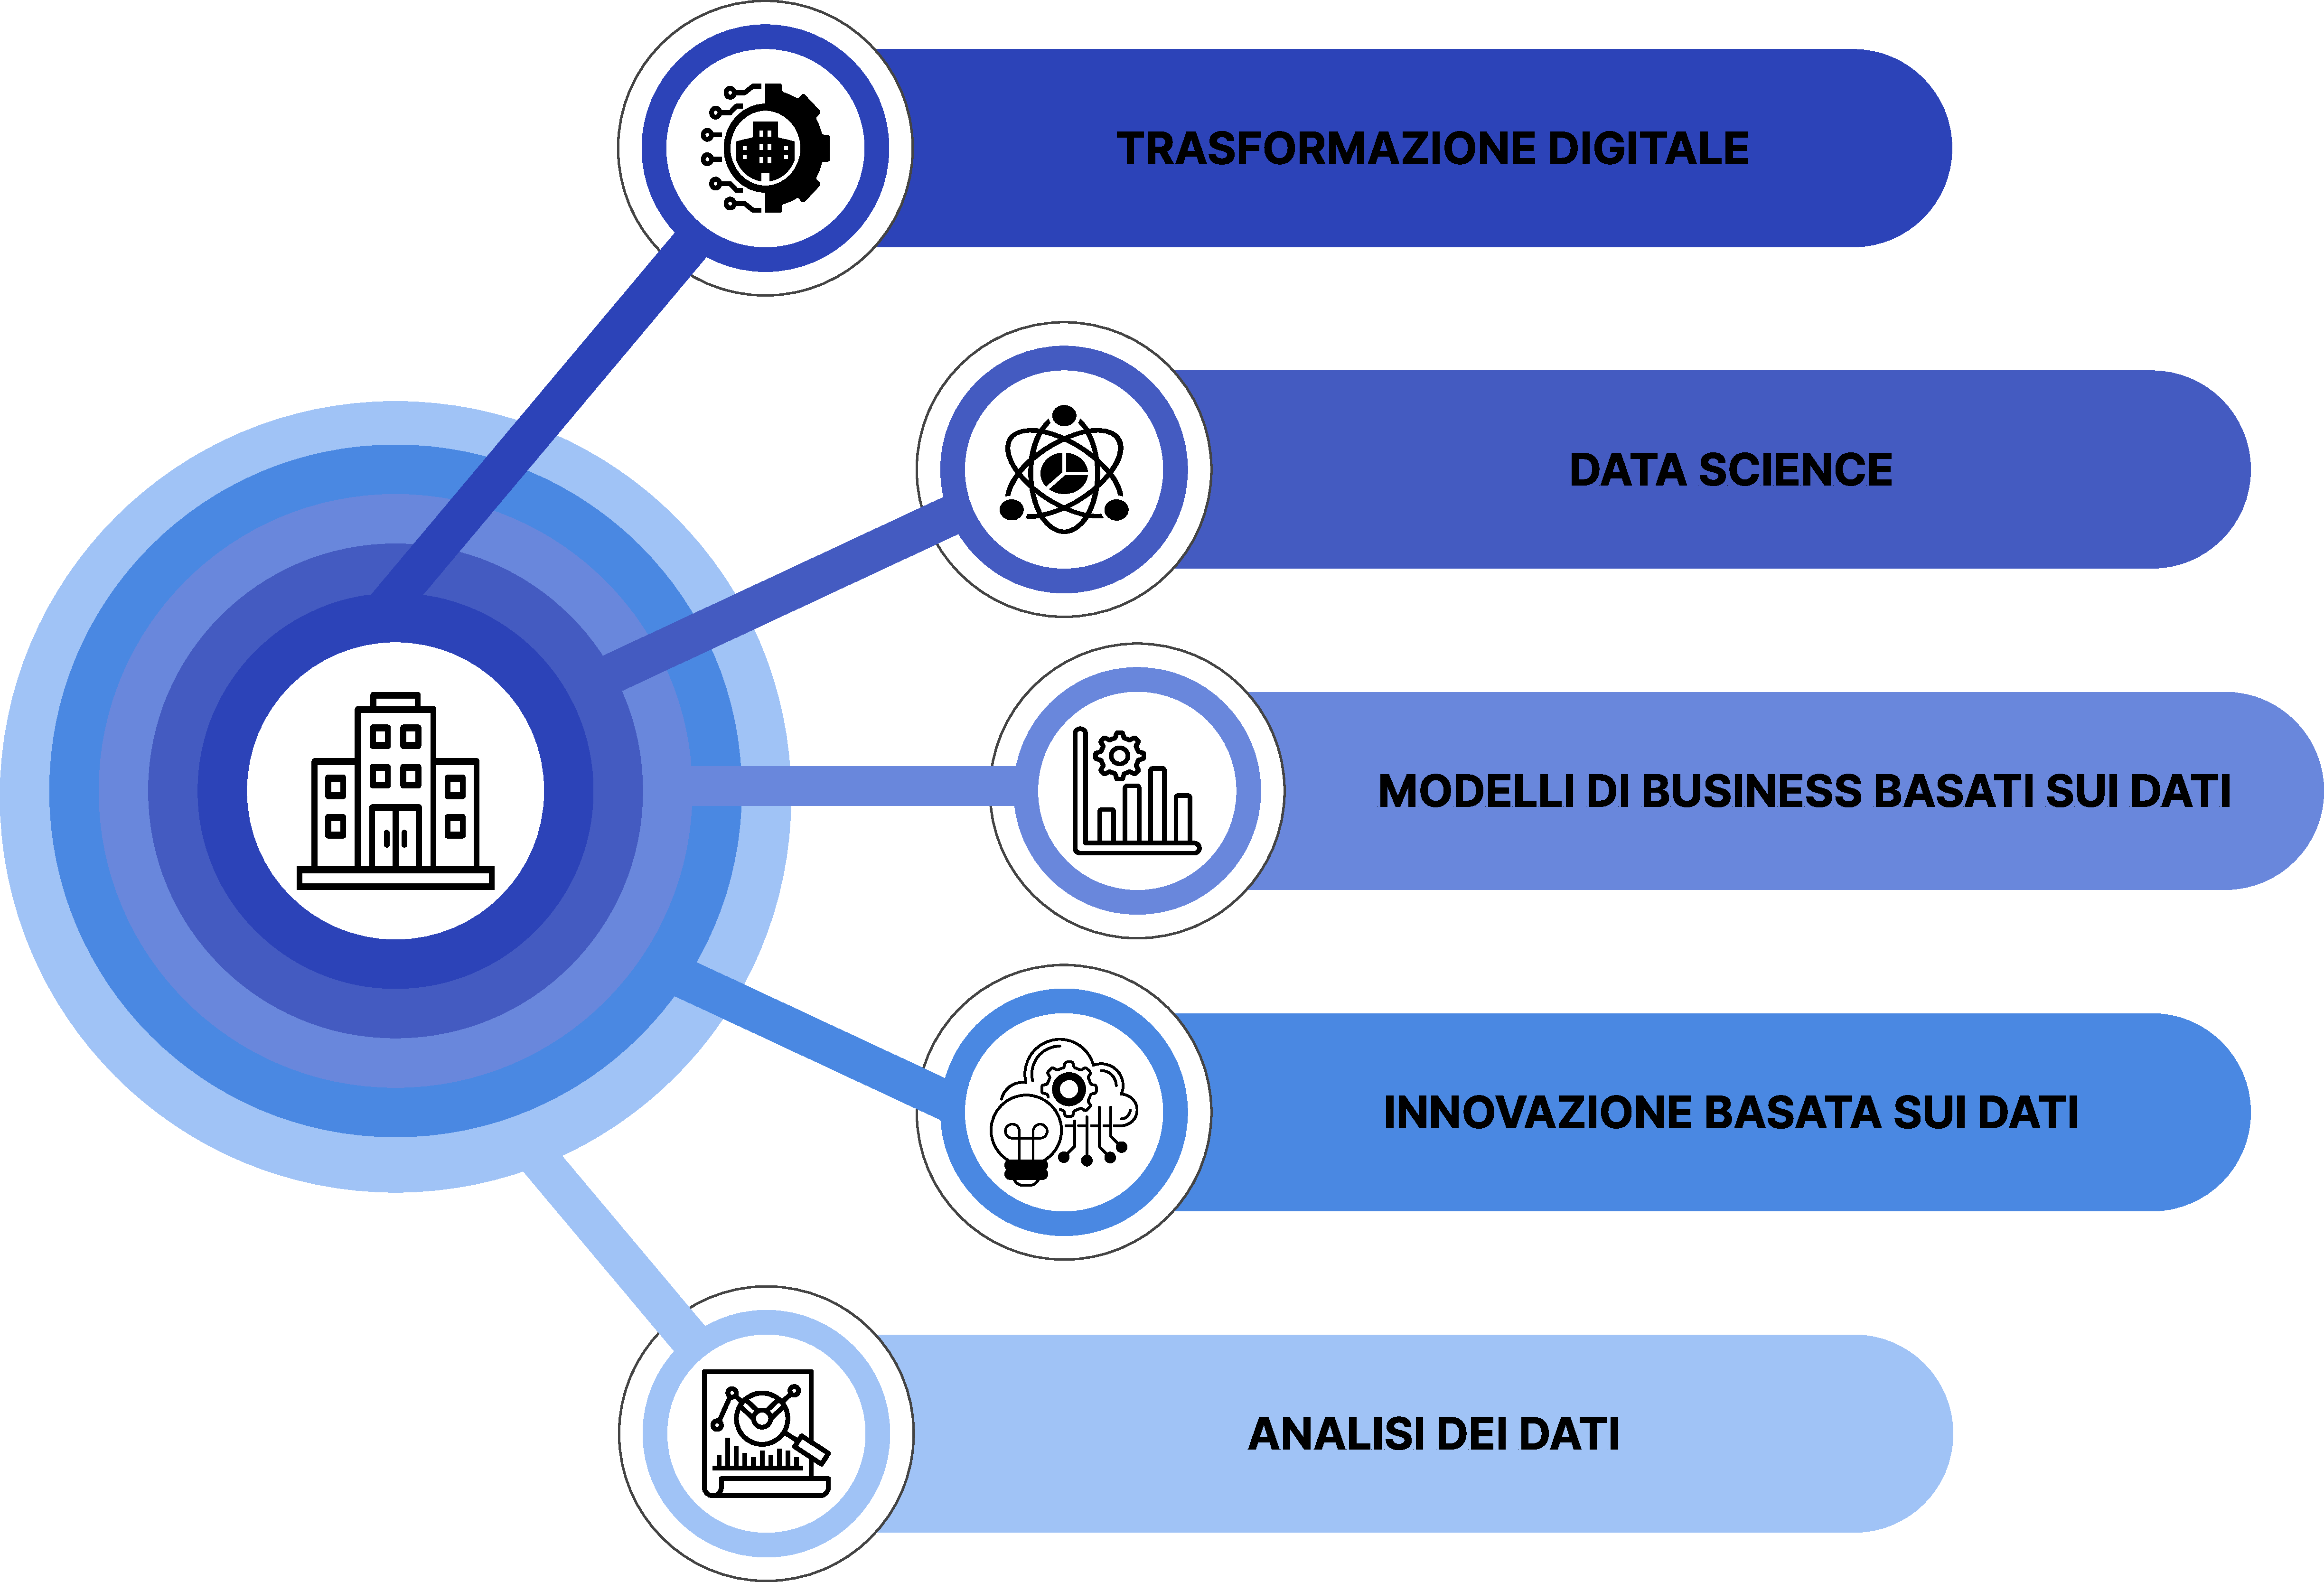
\includegraphics[width=0.75\linewidth]{figure/capitolo_1/Data-Driven company key points.pdf}
    \caption{Punti chiave delle aziende Data-Driven oriented}
    \label{fig:Data-Driven company key points}
\end{figure}

\section{Data Governance}
In un mondo come quello odierno in cui i dati sono uno degli asset di maggior valore, poterli gestire in modo efficace ed efficiente diventa fondamentale in qualsiasi ambito e a qualsiasi livello. Proprio per tale motivo l'Unione Europea ha presentato il documento \textit{Data Governance Act}\footnote{Il \textit{Data Governance Act} è una legge che mira a rendere disponibili più dati, regolando il riutilizzo di dati pubblici/protetti, incrementandone la condivisione attraverso una regolamentazione di nuovi intermediari e incoraggiandone l'adozione a scopi altruistici.} \cite{europe_data_governance_act}.

La \textbf{governance dei dati} (\textit{Data Governance, DG}) promuove la disponibilità, la qualità e la sicurezza di questi all'interno di un'azienda attraverso diverse policy e standard. Questi processi determinano i proprietari, le misure di sicurezza e gli usi previsti per i dati. Nel complesso, l'obiettivo della DG è mantenere dati di alta qualità che siano sicuri e facilmente accessibili per ottenere informazioni aziendali più approfondite \cite{ibm_data_governance}.
Più precisamente, secondo la definizione di Gartner «La governance dei dati è la specificazione dei diritti decisionali e un quadro di responsabilità per garantire il comportamento appropriato nella valutazione, creazione, consumo e controllo dei dati e delle analisi» \cite{gartner_data_governance_definition}.

\subsection{Domini della Data Governance}
Come espresso sopra, definire una governance dei dati all'interno di un'azienda permette di indicare chi detiene i diritti decisionali e le responsabilità riguardo gli asset dell'azienda in questione. Pertanto, è importante identificare quali sono i \textit{domini decisionali} di applicabilità in modo da assegnare correttamente le responsabilità e i doveri alle persone nel modo più consono. 

Tali domini, riportati nella figura \ref{fig:Data Governance Dominions}, sono: \textit{principi dei dati}, \textit{qualità dei dati}, \textit{metadati}, \textit{accesso ai dati} e \textit{ciclo di vita dei dati}. Più precisamente, i principi dei dati sanciscono i confini per l'uso degli asset dei dati che riguardano gli standard aziendali (stabilendo la direzione per tutti gli altri domini decisionali). La qualità dei dati rifinisce la base per come i dati debbano essere interpretati (sfruttando i metadati) e siano accessibili agli utenti (accesso ai dati). Infine, la decisione sul ciclo di vita dei dati definisce la loro produzione, conservazione e ritiro, svolgendo un ruolo fondamentale nell'operazionalizzare i principi dei dati nell'ambito delle infrastrutture IT \cite{data_governance_activities}.

\begin{figure}[!h]
    \centering
    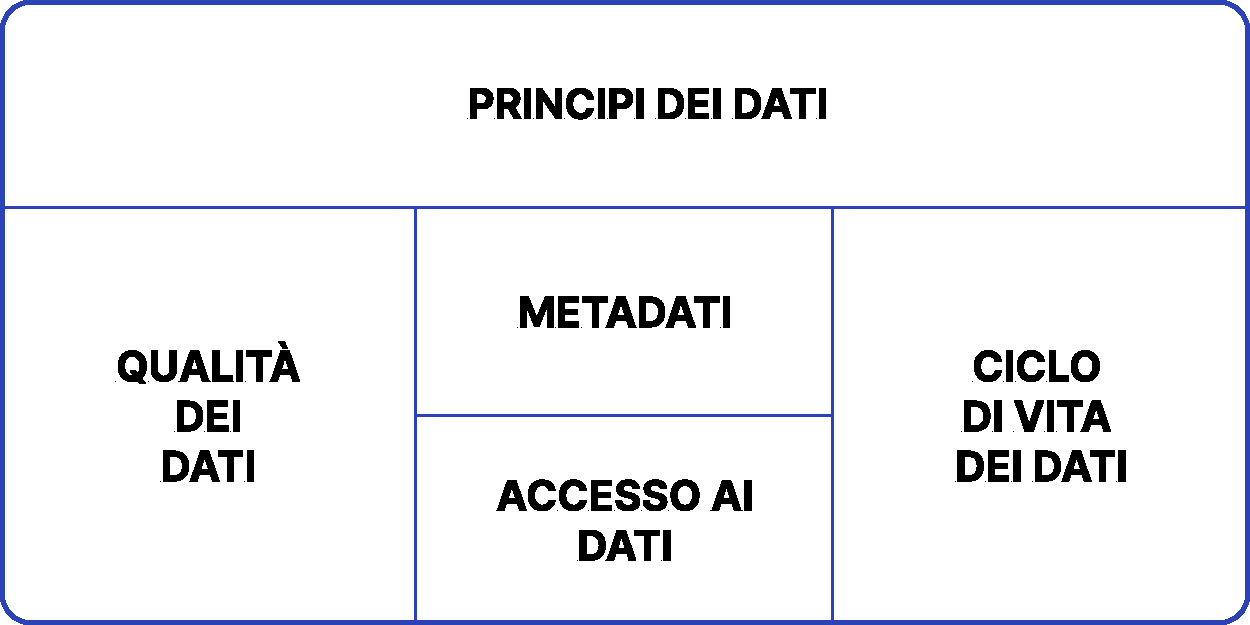
\includegraphics[width=0.75\linewidth]{figure/capitolo_1/Data Governance Dominions.pdf}
    \caption{Domini della Data Governance}
    \label{fig:Data Governance Dominions}
\end{figure}

\subsection{Vantaggi Della Governance Dei Dati}

Di seguito sono riportati i vantaggi che una corretta governance dei dati può comportare all'interno di un'azienda \cite{google_data_governance}:
\begin{itemize}
    \item Prendere decisioni migliori in minor tempo. I dipendenti di un'azienda acquisiscono i dati di cui necessitano per raggiungere e assistere i clienti, progettare e migliorare prodotti e servizi, sfruttando eventuali occasioni.
    \item Migliorare la gestione dei costi. I dati aiutano a gestire le risorse più efficacemente. Grazie ad una corretta gestione sarà inoltre possibile eliminare possibili duplicazioni dei dati, risparmiando spazio e soldi.
    \item Migliorare le conformità normative. Il costante cambiamento del mondo delle leggi e conformità da seguire rende ancora più importante per le organizzazioni una gestione solida e sicura in tale ambito, diminuendone i rischi.
    \item Guadagnare maggiore fiducia da parte dei clienti. La creazione di un sistema preciso, corretto e ben gestito permette alle aziende di avere un impatto più positivo e rassicurante agli occhi delle persone con cui deve interagire.
    \item Gestire i rischi in modo più semplice. Adoperando una governance corretta è possibile aumentare la sicurezza sull'esposizione dei dati sensibili, sulla violazione della sicurezza da parte di malintenzionati.
    \item Consentire a più persone l'accesso ad una maggiore quantità di dati. Una governance ben strutturata permette ad un numero maggiore di utenti di accedere ai dati per loro necessari in minor tempo.
\end{itemize}

\section{Obiettivo della tesi}
La seguente tesi ha sancito una collaborazione diretta tra l'Università degli Studi di Salerno, in particolare con il Dipartimento di Informatica e l'azienda ``Acca Software'' con sede a Bagnoli Irpino. Quest'ultima è il leader italiano del \textit{Building Information Modelling} (BIM) e del software tecnico per l'edilizia, l'ingegneria e l'architettura. L'azienda fornisce servizi a livello internazionale con una suite di software dedicati ai molteplici aspetti relativi alla costruzioni: dalla progettazione, fino alla manutenzione. Nel contesto di un mercato edilizio in continua evoluzione e fortemente interconnesso a livello globale, la qualità dell'assistenza emerge come elemento chiave per il successo di un'azienda. Il nostro studio rappresenta un impegno significativo nel campo dello sviluppo software, mirato a potenziare il settore del supporto tecnico.

L'iniziativa si pone l'obiettivo ambizioso di creare soluzioni software all'avanguardia, sfruttando le tecnologie emergenti legate ai Big Data mirando a fornire all'azienda gli strumenti necessari per una governance dei dati efficiente, permettendo una visione chiara e dettagliata delle informazioni cruciali. Ciò non solo facilita la presa di decisioni tempestive ma contribuisce anche a ottimizzare le risorse, garantendo un'allocazione dinamica delle risorse in base alle esigenze specifiche delle diverse aree di assistenza.

\section{Struttura della tesi}
Questa tesi può essere strutturata nel seguente modo:

\begin{itemize}
    \item \textbf{Capitolo 2}: Una visione generale relativa alle definizione del concetto di Big Data, e le relative caratteristiche da rispettare.
\end{itemize}
\chapter{Background}
\label{ch:Background}

L'incremento di quantità, la possibilità di ridurre rischi e permettere di avere una previsione sulle possibili tendenze di mercato, migliori prestazioni in ambito dei processi decisionale e la presa di coscienza da parte delle aziende su tutti i benefici acquisibili migrando il proprio sistema in un orientamento data-driven. Questi sono solo alcune delle motivazioni che hanno portato i dati a incrementare il proprio valore e importanza all'interno del mondo. Per questa ragione, con il tempo sono state diverse le tecnologie e i processi applicati a quest'ultimi per poter migliorare la loro gestione ed efficienza (e di conseguenza il valore da loro ricavabile). I più importanti tra questi sono i \textit{Big Data}, i \textit{Data Warehouse} e l'\textit{Analisi dei dati}.

\section{I Big Data}

Come accennato in precedenza le esigenze di salvataggio e gestione dei dati sono diventate sempre più importati, proprio per tale motivo ha guadagnato importanza a sua volta anche il mondo dei \textit{Big Data}. Ovvero il campo emergente in cui l'evoluzione del mondo e della sua tecnologia offre nuovi modi per recuperare il valore dalla marea di informazioni generate. La capacità di gestire efficientemente le informazioni e di estrarre conoscenza da quest'ultime è diventato un vantaggio sempre più importante a cui ogni azienda aspira. Di conseguenza, molte compagnie si stanno ponendo come obiettivotanto da farlo diventare anche il proprio core business, la capacità di raccogliere e analizzare i dati, così da ricavarne il maggior numero di informazioni utili possibili. L'adozione della tecnologia dei Big Data nell'ambito delle compagnie non può più definirsi una scelta opzionale, bensì una necessità obbligata per sopravvivere ed ottenere un vantaggio competitivo \cite{new_horizon_for_a_data_driven_economy}.

Ciò è dovuto al fatto che senza informazioni che possano considerarsi adeguate (definite tali poiché consentirebbero di svolgere scelte corrette dettate dalla conoscenza ricavata dalla lettura di tali dati), difficilmente si potrebbe ottenere una strategia vincente. I Big Data sono ciò che permette di svolgere questo compito al meglio, trattandosi di beni da cui è possibile estrarre moltissime informazioni che poi potranno essere impiegate per prendere le decisioni nel miglior stato di conoscenza possibile \cite{iusitinere_big_data}.

Ad avvalorare tali affermazioni, la Acumen Research Consulting (ARC), fornitore globale di servizi di market intelligence e di consulenza per le tecnologie dell'informazione, ha svolto un analisi del mercato dei Big Data relativo al 2021. La Figura \ref{fig:Global-Big-Data-Market} mostra i risultati che hanno attribuito ai Big Data un valore complessivo di 165,5 miliardi di dollari. Inoltre, a seguito di approfonditi studi, è stato previsto un incremento del valore fino a 473,6 miliardi nel 2030 dovuto ad un CAGR\footnote{Il \textit{Compound Annual Growth Rate} (\textit{CAGR}), o \textit{Tasso di crescita annuale composto}, corrisponde alla crescita percentuale media di una grandezza in un lasso di tempo \cite{borsa_italiana_cagr}.} del 12,7\% \cite{acumen_big_data_market}.

\begin{figure}[H]
    \centering
    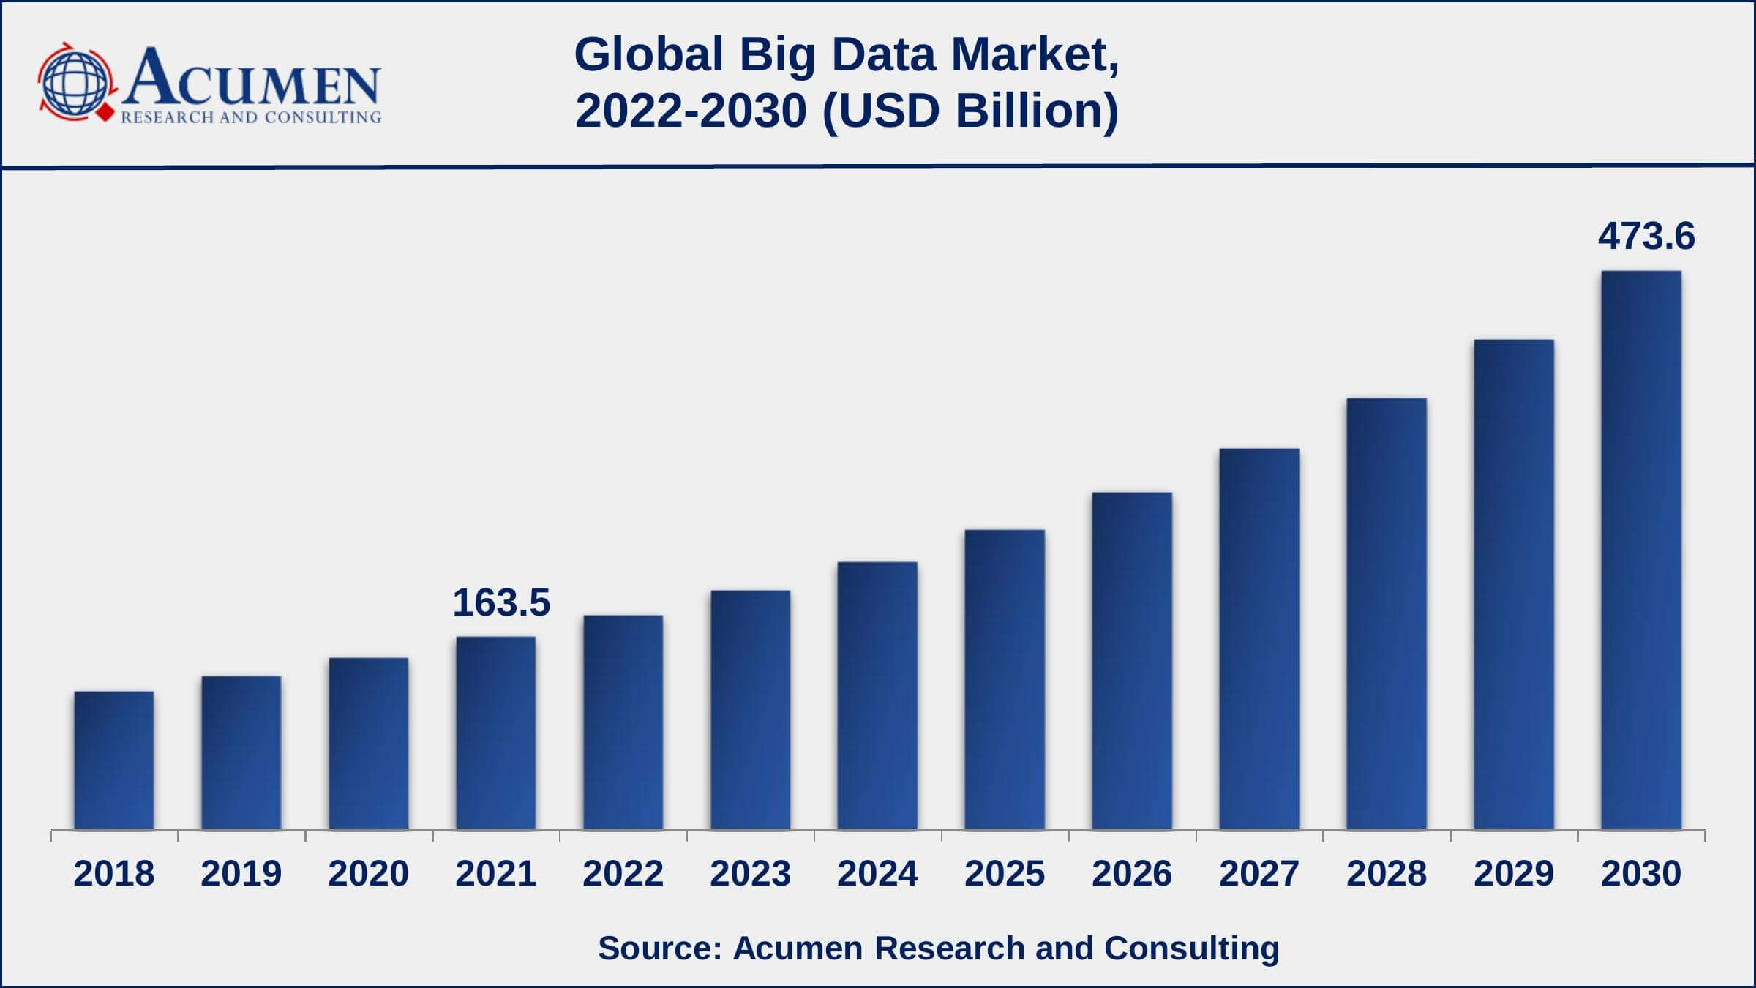
\includegraphics[width=0.7\linewidth]{figure/capitolo_2/Global-Big-Data-Market.pdf}
    \caption{Valore del mercato globale dei Big Data}
    \label{fig:Global-Big-Data-Market}
\end{figure}

\subsection{Definizione di ``Big Data''}

Poiché il dominio dei Big Data è molto eterogeneo, non è ancora possibile evidenziare l'esistenza di una definizione univoca capace di rappresentare tutti i contesti di utilizzo. Per garantire un'analisi completa, abbiamo esaminato le definizioni più pertinenti seguendo le linee guida proposte da Garousi et al. \cite{GAROUSI}. Questo studio ha coinvolto l'esame sia della letteratura ``grigia'' che di quella ``bianca'', includendo sia le pubblicazioni scientifiche che quelle non pubblicate.

Facendo ciò ci è stato possibile comprendere come, anche senza un vero e proprio riferimento ad una definizione ufficiale, molti sono stati i riferimenti eterogenei al mondo dei Big Data. Per poter capire effettivamente cosa siano i Big Data bisogna quindi adoperare una definizione ufficiale, purtroppo però ad oggi non è stata ancora creata. Per questo motivo, di seguito sono riportate le più rilevanti e significative definizioni pubblicate nel tempo.

\begin{longtable}{|p{11cm}|p{3cm}|}
    \hline
    \textbf{Definizione} & \textbf{Autore} \\
    \hline
    \endfirsthead
    %\label{tab:big_data_definitions} \\
    %\caption{Definizioni di Big Data} \\

    \multicolumn{2}{c}%
    {{\bfseries Tabella \thetable{} continua dalla pagina precedente}} \\
    \hline
    \textbf{Definizione} & \textbf{Autore} \\
    \hline
    \endhead

    \hline \multicolumn{2}{|r|}{{Continua nella pagina successiva}} \\ \hline
    \endfoot

    \hline
    \endlastfoot

    «I Big Data sono risorse informative ad alto volume, alta velocità e/o alta varietà che richiedono nuove forme di elaborazione per consentire una migliore presa di decisioni, scoprire nuove intuizioni e ottimizzare i processi.» 
    & Laney Doug (2001) \cite{laney_3d_data_management}\\
    \hline
    «Quando le dimensioni dei dati stessi diventano parte del problema e le tecniche tradizionali per lavorare con i dati perdono efficacia.» 
    & Mike Loukides (2010) \cite{loukides_data_science}\\
    \hline
    «Dati le cui dimensioni ci costringono a guardare oltre i metodi collaudati e consolidati in quel momento.» 
    & Jacobs Adam (2009) \cite{jacobs_big_data}\\
    \hline
    «Le tecnologie Big Data rappresentano una nuova generazione di tecnologie e architetture progettate per estrarre valore in modo economico da volumi molto ampi di dati di varie tipologie, consentendo la cattura ad alta velocità, la scoperta e/o l'analisi.» 
    & IDC (2011) \cite{idc_big_data}\\
    \hline
    «I Big Data sono un insieme enorme di dati complessi che richiedono metodologie, strumenti e competenze atte a gestirli, processarli, estrarli ed analizzarli.» 
    & Elisa Iandiorio (2021) \cite{iandorio_big_data}\\
    \hline
    «Una raccolta di insiemi di dati grandi e complessi che possono essere elaborati solo con difficoltà utilizzando strumenti di gestione di database normalmente disponibili.» 
    & Mike 2.0. (2014) \cite{mike_big_data}\\
    \hline
    «Il termine “Big Data” comprende l'uso di tecniche per catturare, elaborare, analizzare e visualizzare potenzialmente grandi insiemi di dati in un periodo di tempo ragionevole non accessibile alle tecnologie informatiche standard.» 
    & NESSI (2012) \cite{nessi_big_data}\\
    \hline
    «I Big Data di solito includono insiemi di dati di dimensioni oltre la capacità dei comuni strumenti software di recuperare, pulire, gestire ed elaborare dati entro un tempo trascorso tollerabile.» 
    & Wikipedia (2023) \cite{wikipedia_big_data}\\
    \hline
    «Insiemi di dati estremamente grandi che possono essere analizzati computazionalmente per rivelare modelli, tendenze e associazioni, specialmente in relazione al comportamento umano e alle interazioni.» 
    & Google dictionary (2023) \cite{google_big_data}\\
    \hline
    «Definiamo i Big Data come un fenomeno culturale, tecnologico e accademico che si basa sull'interazione tra: (1) Tecnologia: massimizzare la potenza di calcolo e l'accuratezza algoritmica per raccogliere, analizzare, collegare e confrontare grandi insiemi di dati. (2) Analisi: trarre vantaggio da grandi insiemi di dati per identificare modelli al fine di formulare affermazioni economiche, sociali, tecniche e legali. (3) Mitologia: la diffusa convinzione che grandi insiemi di dati offrano un livello superiore di intelligenza e conoscenza che può generare intuizioni che in passato erano impossibili, con l'aura di verità, oggettività e precisione.» 
    & danah boyd, Kate Crawford (2012) \cite{routledge_big_data}\\
    \hline
\end{longtable}

\begin{figure}[H]
    \centering
    
\includegraphics[width=0.8\linewidth]{figure/capitolo_2/Big_Data.pdf}
    \caption{I Big Data}
    \label{fig:Big_Data}
\end{figure}

Naturalmente, queste sono solamente le definizioni identificate come le più rilevanti o anche discordanti tra loro, ma non tutte quelle esistenti. Ciò permette di apprendere come, per quanto non esista una definizione standard, tra tutte quelle esistenti create arbitrariamente dagli studiosi, a seguito di ampie ricerche, siano presenti delle caratteristiche comuni. Perciò, da tali tratti distintivi è possibile affermare che:

\begin{center}
\textit{Il termine Big Data fa riferimento ad un processo adoperante un insieme di dati, anche eterogenei fra loro, la cui dimensione, complessità e velocità di acquisizione ne rendono difficile la gestione, in tempi accettabili, attraverso strumenti e processi tradizionali; tuttavia, grazie ad apposite risorse (personale, hardware e software) tale processo permette di svolgere una gestione ed analisi dei dati tale da ricavare valore da questi in quantità, qualità e tempistiche prima impensabili.}
\end{center}

Quindi, è possibile semplificare il concetto dicendo che con l'espressione “Big Data” si indica la raccolta di una grande mole di dati digitali che, per acquisire valore, richiedono l'utilizzo di specifiche infrastrutture, metodologie di gestione e modelli di analisi. Come è possibile dedurre, il motivo per cui non è stato possibile creare una definizione specifica e che potesse essere assoluta è dovuto al concetto stesso di Big Data. Esso dipende principalmente dal fatto che si parla di una gestione ed analisi di dati che non sarebbe applicabile con tecnologie comuni, con l'evoluzione di quest'ultime dovute al passare degli anni le capacità di elaborazioni migliorerebbero e quindi ciò che era considerato Big Data in passato potrebbe non essere considerato tale oggi o in futuro. Proprio per questo motivo la definizione di Big Data deve essere generica, relativa e dinamica data la sua possibile continua evoluzione.

Sicuramente sentendo le parole “Big Data” una delle prime associazioni che si hanno nella propria mente è quella di un grande volume di dati, tuttavia se si volesse conoscere la quantità precisa per comprendere quando effettivamente si stia parlando di Big Data ciò non sarebbe possibile per due motivi:

\begin{itemize}
    \item sono definiti “grandi” non solo per il loro volume, ma anche per la varietà e la complessità che li contraddistingue;
    \item per lo stesso motivo del “problema” che affligge la definizione del termine Big Data, non è possibile quantificare il volume minimo per parlare di Big Data poiché le dimensioni che si hanno al giorno d'oggi, come abbiamo potuto apprendere in precedenza, non sono paragonabili a quelle passate o future.
\end{itemize}

\subsection{Caratteristiche}

A seguito del proprio studio sul fenomeno dei Big Data, Doug Laney elaborò un nuovo modello in grado di definire quali fossero le loro caratteristiche. Prese il nome di “\textbf{Modello delle 3V}”, poiché pone i 3 concetti di \textit{Volume, Velocità e Varietà} alla base della definizione di Big Data (riportata nella tabella \ref{tab:big_data_definitions}). Col passare degli anni e con l'evoluzione del fenomeno tale modello è stato integrato con altre quattro proprietà in grado di definire e interpretare ancor di più nello specifico le caratteristiche di ogni dato, ovvero \textit{Valore, Veridicità, Valenza e Visualizzazione}. (È importante precisare che risulta difficile isolare le singole caratteristiche poiché esiste una forte legame tra di loro.) Di seguito sono riportate le definizioni delle caratteristiche elencate \cite{agcom_big_data}.
\begin{itemize}
    \item \textbf{Volume} (\textit{Volume}). Il volume rappresenta la caratteristica che più facilmente si può accostare ai Big Data; però come detto in precedenza numerosi sono stati gli studi che cercano di misurare tale caratteristica, tuttavia è stata riscontrata l'impossibilità di conoscerne il preciso ammontare.
    \item \textbf{Varietà} (\textit{Variety}). La varietà fa riferimento all'eterogeneità delle fonti sorgenti dei dati, dei loro formati, da cui vengono acquisite le informazioni e della rappresentazione e analisi dei dati immagazzinati.
    \item \textbf{Velocità} (\textit{Velocity}). La velocità è connessa alle tempistiche con cui le banche dati vengono alimentate, in particolare alla alta frequenza con cui i dati circolano da un punto di origine a uno di raccolta. Tuttavia, la velocità non riguarda esclusivamente il flusso di origine dei dati, ma anche la necessità di processare questi in maniera rapida e per prendere decisioni ad un ritmo sempre più veloce, spesso anche in tempo reale.
    \item \textbf{Valore} (\textit{Value}). Il valore corrisponde alla capacità di estrarre/ricavare dai dati il loro relativo valore economico, o più precisamente le informazioni che possano diventare un valore aggiunto per svolgere decisioni, di qualsiasi genere o ambito di riferimento, che comportino un guadagno economico. 
    \item \textbf{Veridicità} (\textit{Veracity}). La veridicità pone l'attenzione sulla rilevanza degli aspetti qualitativi legati ai dati e, di conseguenza, alla fiducia che in essi si può riporre. In altri termini, la veridicità garantisce che i dati siano accurati; ciò comporta la necessità di impedire l'accumulo nei sistemi di dati che non siano “utili”.
    \item \textbf{Variabilità} (\textit{Variability}). Per prima cosa bisogna sottolineare che la variabilità è differente dalla varietà. I significati e le interpretazioni di questi agglomerati di dati grezzi dipendono molto dal loro contesto. Quando si tratta di analizzare le impressioni, questo è fondamentale. Gli algoritmi devono essere in grado di comprendere il contesto in cui operano e decifrare il significato preciso di ogni parola nel loro specifico ambiente. La variabilità illimitata dei Big Data presenta quindi una sfida di decodifica unica se si vuole sfruttare tutto il suo valore.
    \item \textbf{Visualizzazione} (\textit{Visualization}). Per visualizzazione dei dati si intende ricavare informazioni sintetiche e renderle di facile comprensione da una vastità di dati, essa rappresenta indubbiamente una delle sfide più ardue da affrontare.
\end{itemize}

\begin{figure}[h!]
    \centering
    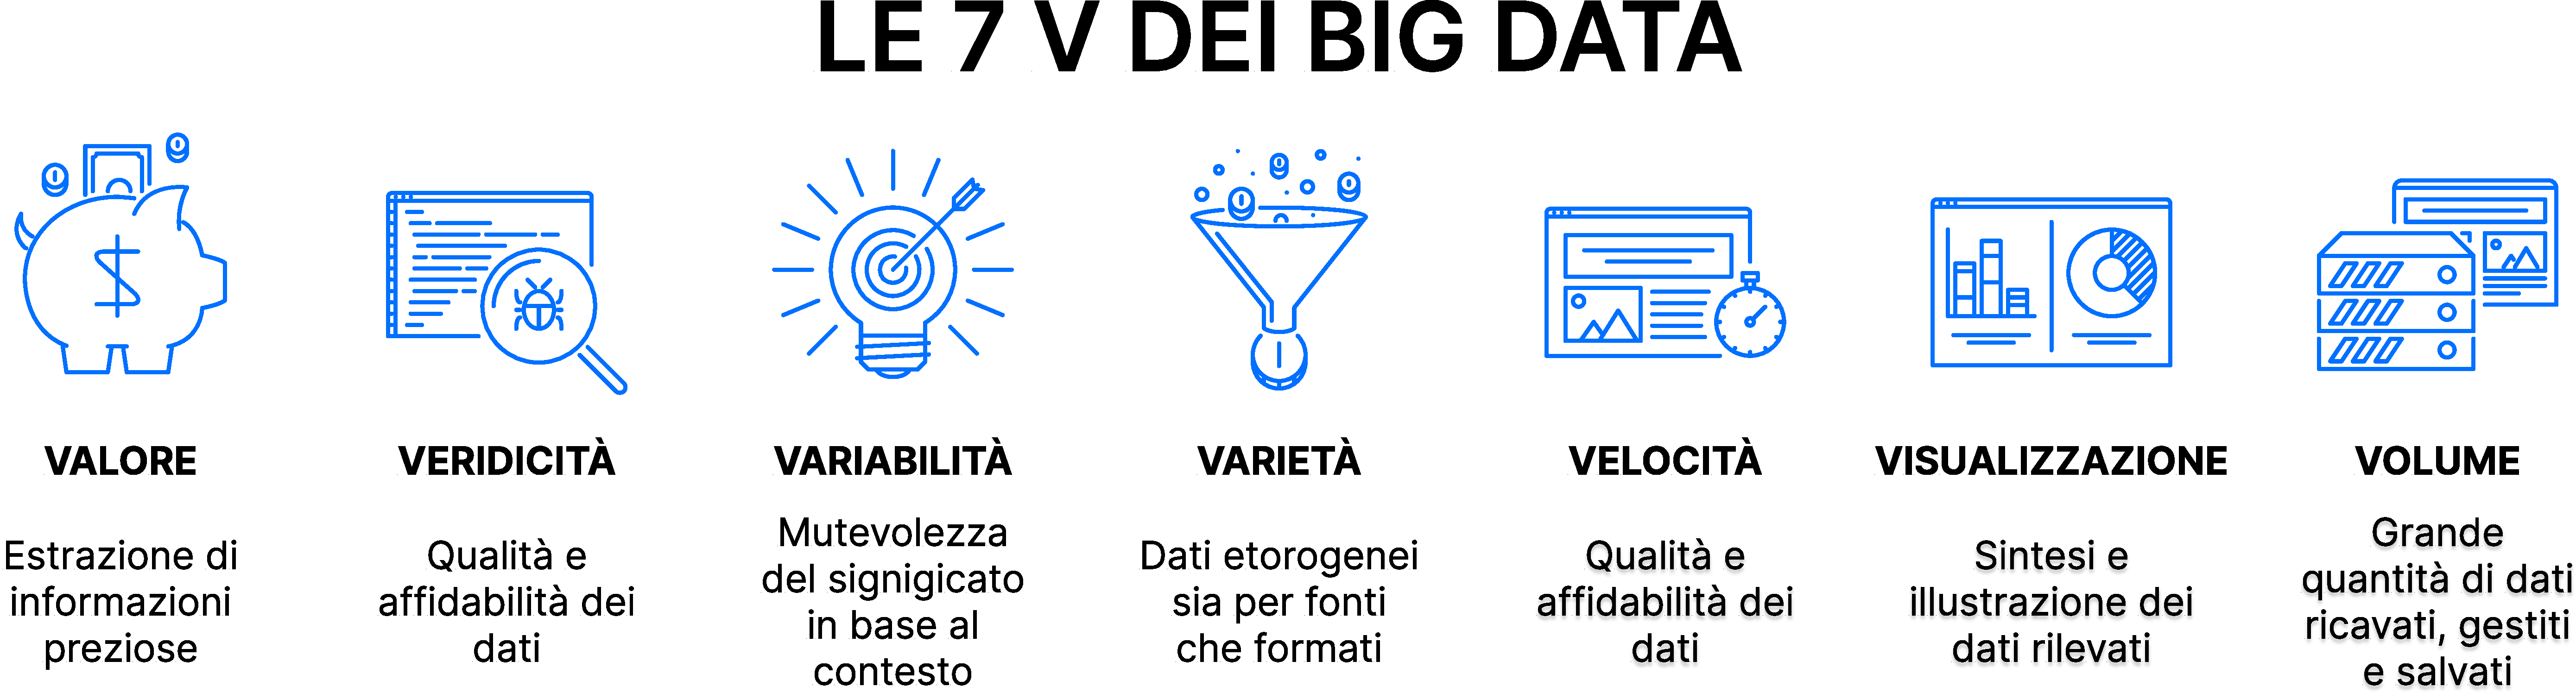
\includegraphics[width=1\linewidth]{figure/capitolo_2/Le 7 V dei Big Data.pdf}
    \caption{Le 7 V dei Big Data}
    \label{fig:Le 7 V dei Big Data}
\end{figure}

\subsection{Strutturazione dei Dati}

Come affermato sopra, una delle caratteristiche dei Big Data è la varietà poiché in un ambiente possibilmente eterogeneo come questo, i dati vengono ricevuti quasi sempre in formati differenti. In base al loro formato, o per meglio dire la loro \textit{struttura}, è necessario adoperare approcci distinti per ottenere le informazioni necessarie.

Quando si parla di \textbf{struttura dei dati} si riferisce ai metodi di organizzazione delle unità di dati all'interno di insiemi più grandi. La creazione e il mantenimento di specifiche strutture di dati aiutano a migliorare l'accesso al valore di quest'ultimi. Man mano che i dati vengono organizzati in modo più elaborato essi diventano più funzionali \cite{theastrologypage_data_structure}.

In base alle necessità, all'architettura del progetto e al loro scopo, i dati possono essere salvati in tre diversi modi:

\begin{itemize}
    \item \textbf{Dati strutturati}. I dati strutturati sono dati la cui struttura è predefinita e quindi rispettano tutti la stessa forma prima di essere inseriti all'interno dell'archivio dati. Ciò permette di avere lo stesso insieme di proprietà per i dati che rispettano il medesimo formato. Tali dati vengono anche chiamati dati relazionali poiché è possibile rappresentarli facilmente in un formato tabellare relazionabile tra loro \cite{geeksforgeeks_big_data_structure}.
    \item \textbf{Dati semi-strutturati}. I dati semi-strutturati sono una tipologia di dati che non è conforme ad una struttura formale di modelli di dati, ma che sfrutta alcuni tipi di tag organizzativi per separare gli elementi semantici che li compongono così da definire delle gerarchie per i campi che contengono le informazioni. Solitamente queste strutture sono adoperate per il salvataggio dei metadati, che contengono delle informazioni strutturate ma non sempre gli stessi campi \cite{magnimind_big_data_structure}.
    \item \textbf{Dati non strutturati}. I dati non strutturati sono il tipo di dati che non aderiscono ad uno schema o insieme di regole definito e quindi si presentano in forme o strutture ignote e diverse tra loro. Questo tipo di dati ha una forma sconosciuta e non può essere archiviato in modi tradizionali o analizzato a meno che non vengano trasformati in un formato strutturato. Proprio per questo motivo la gestione di tali dati è un compito impegnativo \cite{altervista_big_data_structure}.
\end{itemize}

Principalmente, i dati contenenti le informazioni vengono salvati in formati strutturati o non strutturati e per questo motivo spesso si incorre nel dubbio sul quale scegliere tra i due formati per il proprio progetto. Di seguito è riportata una tabella che mostra le differenze fra le due tipologie di dati \cite{analytixlabs_big_data_structure}.

\begin{longtable}{|p{2cm}|p{6cm}|p{6cm}|}
    %\label{tab:data_structure_differences} \\
    % \caption{Differenze tra dati strutturati e non strutturati} \\
    \hline
    \textbf{Ambito di paragone} & \textbf{Dati Strutturati} & \textbf{Dati Non Strutturati} \\
    \hline
    \endfirsthead

    \multicolumn{3}{c}%
    {{\bfseries Tabella \thetable{} continua dalla pagina precedente}} \\
    \hline
    \textbf{Ambito di paragone} & \textbf{Dati Strutturati} & \textbf{Dati Non Strutturati} \\
    \hline
    \endhead

    \hline \multicolumn{3}{|r|}{{Continua nella pagina successiva}} \\ \hline
    \endfoot

    \hline
    \endlastfoot

    Struttura & I dati strutturati nei Big Data si basano su RDBMS e seguono una struttura a righe-colonne. &  I dati non sono organizzati in un modo definito, per questo motivo non funzionano con alcun set di modelli di dati. \\
    \hline
    Fonti & Provengono principalmente da database relazionali, sistemi di gestione, siti web, applicazioni, dati finanziari, archivi dati, sensori e dispositivi IoT. & Provengono principalmente da file di testo, immagini, video, audio, documenti PDF, e-mail, social media, log e dati di tracciamento, documenti di elaborazione e bot di assistenza.\\
    \hline
    Formati & I loro possibili formati di origini sono: CSV, Excel, DB Relazioni, XML, Parquet ed Avro. & I loro possibili formati di origini sono: TXT, PDF, JPEG, PNG, MP3 e MP4.\\
    \hline
    Modelli & Modello che rispetta una struttura predefinita prima di essere salvati nell'archivio dati. & Sono memorizzati nel proprio formato originale senza essere elaborati finché non eseguiti.\\
    \hline
    Salvataggio & I dati vengono salvati in un formato tabellare e richiedono meno spazio di archiviazione. & Questi dati vengono archiviati come file multimediali o database NoSQL, richiedendo maggiore spazio di archiviazione.\\
    \hline
    Formato & Segue uno schema rigido che fornisce sia coerenza che efficienza. & Non segue una struttura costante e per questo è incoerente.\\
    \hline
    Facilità di analisi & Esistono diversi strumenti di analisi rodati per il recupero, la gestione e l'analisi dei dati. & Gli strumenti per il recupero, la gestione e l'analisi dei dati sono ancora in fase di sviluppo.\\
    \hline
\end{longtable}

In altre parole, analizzando le differenze riportate nella tabella precedente, la scelta di adoperare uno dei due formati di dati dipende da quale sia lo scopo e soprattutto la tipologia di informazioni che si vorrebbero salvare. Non esiste un formato che prevale sull'altro in qualsiasi caso, ma solamente in base alla propria esigenza.

\begin{figure}[h!]
    \centering
    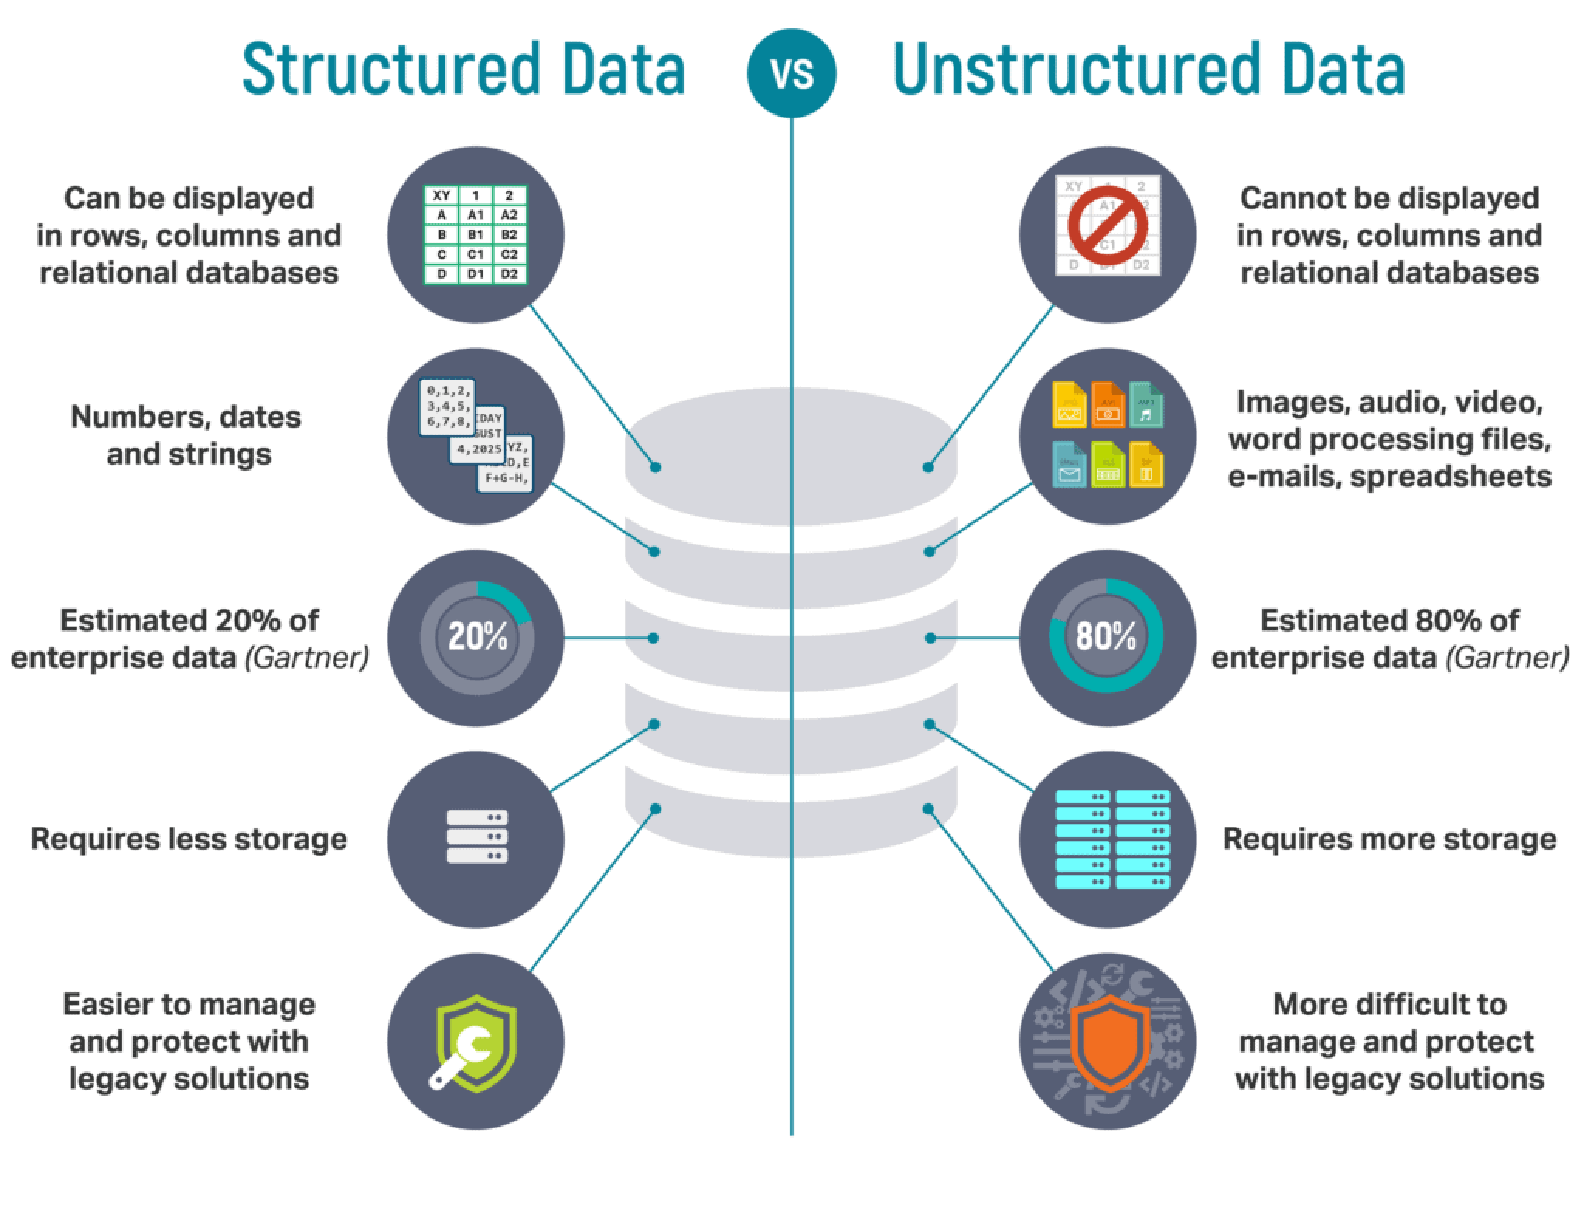
\includegraphics[width=0.55\linewidth]{figure/capitolo_2/structured-data-vs-unstructured-data.pdf}
    \caption{Differenze tra dati strutturati e dati non strutturati}
    \label{fig:structured-data-vs-unstructured-data}
\end{figure}

\subsection{Vantaggi e Problematiche dei Big Data}

I Big Data rappresentano il fattore produttivo chiave in un'economia data-driven; molti sono gli ambiti, sia privati che pubblici, in cui l'utilizzo di tecniche di analisi di Big Data ha permesso di creare nuovi servizi, migliorare quelli esistenti, innovare i processi produttivi e distributivi, rendere l'offerta di tutti i prodotti e servizi, migliorare quelli esistenti, innovare i processi produttivi e distributivi, rendere l'offerta di tutti i prodotti e servizi (anche non digitali) più rispondenti alle esigenze dei consumatori e cittadini. Tuttavia, benché stimolante, l'analisi dei Big Data è un'operazione complessa. I data scientist si occupano dell'analisi dei dati per offrire all'azienda informazioni e raccomandazioni utili e i data engineer sono responsabili di identificare, assemblare e gestire gli strumenti necessari in un flusso di dati. Ogni singola fase rappresenta delle sfide in termini di integrazione, capacità di storage e riduzione dei budget IT \cite{redhat_big_data}.

Pertanto di seguito sono riportate alcune delle problematiche da considerare se si ha l'intenzione di predisporre un sistema per l'applicazione dei Big Data \cite{microsoft_big_data}:

\begin{itemize}
    \item \textit{Organizzazione e accessibilità dei dati}. La principale problematica associata ai Big Data consiste nel capire come gestire il volume di informazioni ottenute affinché pervengano correttamente nelle applicazioni.
    \item \textit{Controllo qualità}. Garantire l'accuratezza e la qualità dei dati può essere difficile e dispendioso in termini di tempo, soprattutto quando tali dati arrivano rapidamente e a volumi molto elevati. Prima di effettuare qualsiasi analisi, occorre assicurarsi che i processi di raccolta, elaborazione e pulizia dei dati siano integrati, standardizzati e ottimizzati.
    \item \textit{Sicurezza dei dati}. Con l'aumento delle violazioni di dati, la protezione di quest'ultimi ha sempre più importanza. Così come il sistema di analisi cresce, aumenta anche la possibilità di riscontrare problemi di sicurezza sotto forma di dati fittizi, fughe di informazioni, problematiche relative alla conformità e alla vulnerabilità del software. Per ridurre alcune di tali preoccupazioni, occorre crittografare i dati e condurre regolarmente controlli di sicurezza.
    \item \textit{Scelta degli strumenti giusti}. Dover scegliere tra i tantissimi strumenti e tecnologie disponibili può creare confusione. Ecco perché è importante provvedere alla formazione, rimanere sempre aggiornati e, se possibile, assumere o consultare uno specialista ove necessario.
\end{itemize}

Una volta mostrate le problematiche a cui fare attenzione per sviluppare un sistema di gestione dei Big Data, è ora importante mostrare quanto siano rilevanti i vantaggi nell'intraprendere questa scelta \cite{oracle_big_data}.

\begin{itemize}
    \item \textit{Sviluppo di prodotti e servizi}. L'analisi dei Big Data consente agli sviluppatori di prodotti di analizzare dati non strutturati, quali le recensioni dei clienti e le tendenze culturali, e di reagire prontamente anche predicendo le eventuali richieste anticipando la domanda della propria utenza.
    \item \textit{Manutenzione predittiva}. I fattori che possono prevedere guasti meccanici possono essere nascosti tra i dati strutturati, riguardanti le informazioni della strumentazione, oppure nei dati non strutturati, riguardanti le informazioni generate da tali dispositivi. Analizzando queste indicazioni di potenziali problemi prima che si verifichino, le aziende possono svolgere la manutenzione in modo più efficiente in termini di costi e tempistiche.
    \item \textit{Customer Experience}. I Big Data consentono di raccogliere dati da social media, visite sui siti web, registri delle chiamate e altre fonti allo scopo di migliorare l'esperienza di interazione tra l'utente e l'azienda. In altre parole, l'analisi di tali dati permette alle organizzazioni di migliorare l'esperienza vissuta dai clienti con il loro brand in modo da ottenere una maggiore soddisfazione da parte dell'utente, che corrisponde a possibili nuovi introiti.
    \item \textit{Frode e conformità}. Gli scenari di sicurezza e i requisiti di conformità sono in continua evoluzione. I Big Data aiutano a identificare i modelli nei dati che indicano frodi e ad aggregare grandi volumi di informazioni per rendere i rapporti normativi molto più veloci. Gli insight generati dall'analisi dei tali dati consentono alle aziende di anticipare il rischio e a prepararsi ad eventuali malevoli imprevisti.
    \item \textit{Efficienza operativa}. L'efficienza operativa potrebbe non essere sempre un argomento innovativo, ma ha molta rilevanza nel mondo dei Big Data. In tale ambito, è possibile analizzare e valutare la produzione, i feedback e i resi da parte dei clienti, e ulteriori fattori per ridurre le interruzioni e anticipare le future richieste. I Big Data possono essere utilizzati anche per migliorare il processo decisionale in linea con l'attuale domanda di mercato.
    \item \textit{Incentivare l'innovazione}. I Big Data possono aiutare ad innovare studiando le interdipendenze tra essere umani, istituzioni, entità e processi e quindi determinando nuovi modi per utilizzare tali insight. Sfruttare gli insight così generati crea infinite possibilità, dal migliorare le decisioni su considerazioni interne a fornire nuovi prodotti e servizi.
\end{itemize}

\subsection{Thick Data}

Come abbiamo potuto comprendere, i Big Data non riescono a mostrare tutte le informazioni che si potrebbero recuperare da una determinata fonte. Per questo motivo, esiste un'altra famiglia di dati che ha la sua rilevanza nel mondo dell'analisi dei dati, ovvero i \textit{thick data}.

I \textbf{thick data} riguardano le informazioni sul significato e le connessioni che le persone attribuiscono ai servizi o alle tecnologie, così come il processo con cui li consumano. L'idea alla base è che l'analisi interpretativa dei dati deve seguire un approccio non solamente quantitativo ma anche qualitativo puntando a ulteriori fattori come quelli esterni ai dati a disposizione. Di seguito è riportata una tabella riepilogativa che permette di comprendere la differenza tra i Big Data ed i thick data \cite{big_data_and_thick_data}.

\begin{comment}
\begin{table}[!ht]
    \centering
    \caption{Differenza tra i Big Data e i Thick Data}
    \begin{tabular}{|l|l|l|}
    \hline|
        \textbf{Caratteristiche} & \textbf{Big Data} & \textbf{Thick Data} \\ \hline
        Formato & Dati in formato numerico. & Dati non numerici, qualitativi formato. \\ \hline
        Volume & Solitamente quantità elevate. & Solitamente quantità basse. \\ \hline
        Metodi di collezione & Documenti digitali, archivio digitalizzato record, streaming di dati, log di trasmissione, dati numerici recuperati da Internet. & Osservazioni e interviste dirette ai partecipanti, focus group, sondaggi a risposta aperta, video registrazioni, dati qualitativi provenienti da Internet \\ \hline
        Analisi & Ricerche di scienziati sociali e computazionali. & Ricerche di antropologi e etnografi. \\ \hline
        Requisito di immersione & Non è necessario che gli analisti siano in loco per analizzare i dati. & Di solito in loco o con l'osservazione diretta online, e immersi nel contesto. \\ \hline
        Ruolo nella soluzione dei problemi & Generare soluzioni a problemi in gran parte noti, generando decisioni automatiche. & Identifica i problemi che contano di più per le parti interessate e testa le soluzioni prima di espanderle. \\ \hline
        Punti di forza & \textit{Scala}: generare insight generalizzabili a un'ampia porzione o a un'intera popolazione. & \textit{Profondità}: identificare ciò che interessa in primo luogo agli stakeholder; dipingere un quadro olistico di determinate esperienze. \\ \hline
    \end{tabular}
    \label{BG vs TD}
\end{table}
\end{comment}

In altre parole, i thick data, analizzando il contesto in cui i dati vengono recuperati, permettono di comprendere le motivazioni che hanno portato le persone a svolgere determinate scelte, ciò permette anche di comprendere quali sono stati i ragionamenti e le sensazioni che hanno portato a prendere una determinata decisione da parte di un utente. Di conseguenza, quando i Big Data vengono combinati con i thick data, è possibile generare un quadro più completo delle esigenze, dei requisiti e delle preferenze dei consumatori.

\begin{figure}[h!]
    \centering
    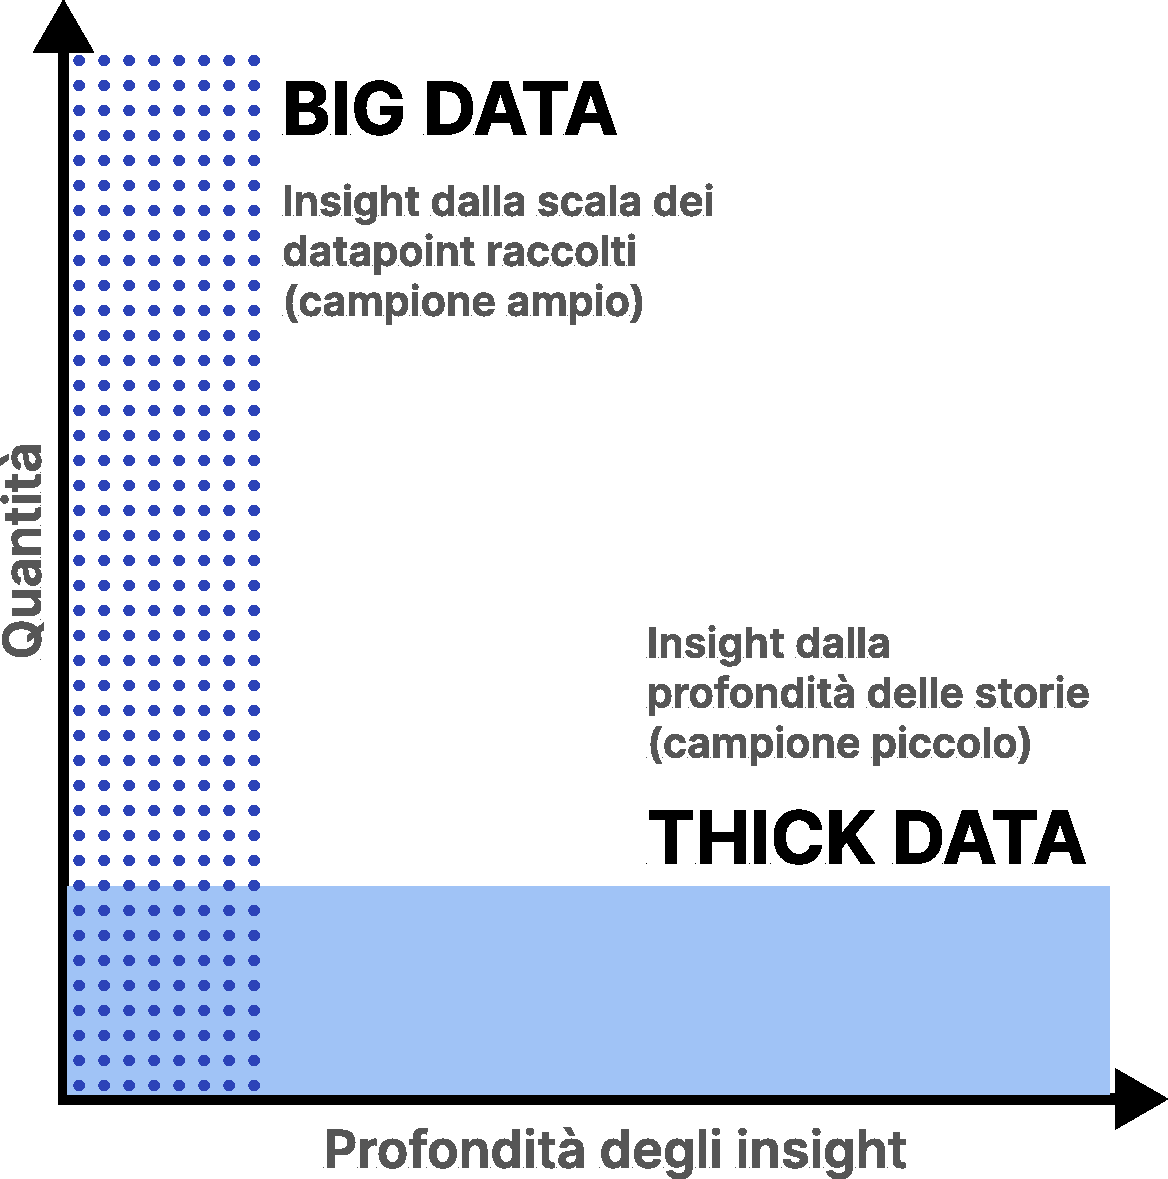
\includegraphics[width=0.5\linewidth]{figure/capitolo_2/Thick and Big Data.pdf}
    \caption{Schema dei Thick e Big Data}
    \label{fig:Thick and Big Data}
\end{figure}

\subsection{Differenza Tra i Big Data e i Dati Tradizionali}

Di seguito è riportata una tabella che permette di descrivere le differenze tra i Big Data e i dati tradizionali \cite{big_vs_traditional_data}.

\begin{comment}
\begin{table}
    \centering
    \begin{tabular}{ccc}
        Caratteristica & Big Data & Dati tradizionali\\
        Dimensioni & Volumi approssimativamente misurati in petabyte, exabyte o zettabyte. & Volumi approssimativamente misurati in gigabyte e terabyte\\
        Organizzazione & Dati, principalmente, grezzi o non strutturati con schemi dinamici & Dati strutturati organizzati in record, file e tabelle, solitamente sono dati relazionali\\
        Architettura & Quasi sempre gestiti adoperando sistemi distribuiti dato il volume e la complessità & Solitamente gestiti adoperando sistemi con strutture centralizzate\\
        Fonti & Derivano da fonti di qualsiasi genere: programmi, social media, dispositivi IoT, ecc. & Derivano in genere da determinati programmi con uno scopo specifico\\
        Analisi & L'analisi può essere svolta sia in modo incrementale che in tempo reale & Analisi incrementale: si verifica un evento, i dati vengono generati, gestiti e poi analizzati\\
    \end{tabular}
    \caption{Differenza tra Big Data e dati tradizionali}
    \label{tab:big_vs_traditional_data}
\end{table}
\end{comment}

I Big Data e i dati tradizionali hanno scopi diversi ma correlati, che ben possono collaborare tra loro.

\section{I Data Warehouse}

Il \textit{data warehousing} ha iniziato il proprio percorso negli anni '70 grazie a William H. Inmon e Ralph Kimball poiché ritenevano che i database basati sui modelli, per quanto efficienti nel trattamento dei dati relazionali, non lo gossero altrettanto per casi di report analitici complessi. Le aziende necessitavano di un'analisi dei dati migliore per prendere decisioni aziendali efficaci e ben ragionate. Ai tempi non esisteva una metodologia di integrazione adeguata disponibile per rappresentare i dati necessari che le compagnie immagazzinavano nei vari sistemi di supporto \cite{researchgate_data_warehouse}.
Per sopperire a tali necessità Inmon e Kimball condussero una ricerca dettagliata sui \textit{sistemi di supporto decisionale} e sui \textit{data warehouse}, sviluppando un loro approccio nella creazione di tali sistemi che permettessero attività di analisi, centralizzando grandi quantità di dati derivanti da più origini e formati.

\subsection{Definizione}

Il padre del termine \textbf{data warehouse} è William H. Inmon che, nel finire degli anni '90, lo definì come «una raccolta di dati orientati al soggetto, integrati, non volatili e varianti nel tempo, finalizzata a supportare le decisioni della direzione aziendale». In quest'ottica, i data warehouse assumono un doppio scopo nella gestione dei dati \cite{inmon_building_the_data_warehouse}:

\begin{itemize}
    \item Possibilità di essere interrogati per recuperare specifiche informazioni necessarie nell'immediato.
    \item Mantenimento dei dati con l'obiettivo di sfruttarli in futuro quando avranno assunto maggior valore.
\end{itemize}

Analizzando meglio la suddetta definizione di Inmon, è possibile affermare che essa si basi su quattro caratteristiche fondamentali che riguardano i dati di cui un data warehouse si compone. Per avere una migliore comprensione del concetto, di seguito sono riportate le spiegazioni di tali caratteristiche \cite{researchgate_data_warehouse_architecture}:

\begin{enumerate}
    \item \textit{Orientati al soggetto}: tutti i dati, ritenuti importanti, relativi ad un determinato argomento vengono raccolti e archiviati come un unico insieme in un formato utile; tali dati vengono presentati in base a soggetti specifici oppure aree di interesse.
    \item \textit{Integrati}: i dati vengono archiviati in modo globalmente accettabile, ovvero rispettando una determinata convenzione cosicché le loro strutture e attributi possano essere coerenti anche indipendentemente dal caso in cui il loro formato originale di archiviazione, dovuto a sistemi operativi eterogenei, siano differenti o addirittura incompatibili.
    \item \textit{Non volatili}: le informazioni ricavabili dai dati archiviati non devono cambiare ogni volta che viene eseguito un processo di recupero o analisi; tali informazioni sono coerenti indipendentemente dal momento in cui vengono richieste al data warehouse.
    \item \textit{Varianti nel tempo}: questa caratteristica, per quanto a primo impatto possa sembrare in contraddizione con la precedente, in realtà la avvalora. Quando si parla di “varianti nel tempo” si intende che le informazioni recuperate possano variare dipendentemente dal periodo in cui vengono recuperate e ciò permette di mantenere una traccia dei cambiamenti avvenuti così che possano descrivere la storia del soggetto a cui si fa riferimento. Ciò naturalmente è possibile inserendo il periodo di riferimento all'interno delle informazioni registrate nei dati salvati e salvando tutti gli stati che li contraddistinguono.
\end{enumerate}

\subsection{Obiettivi dei Data Warehouse}
Per comprendere meglio cosa sono i data warehouse è utile fare una ricapitolazione di quali sono gli obiettivi per cui vengono utilizzati \cite{kimball_the_data_warehouse_toolkit}.

\begin{itemize}
    \item \textit{Rendere le informazioni facilmente accessibili}. I dati devono essere intuitivi e ovvi per l'analista e non solo per lo sviluppatore. Le strutture e le etichette dei dati dovrebbero rappresentare i processi mentali e il vocabolario dell'azienda. 
    \item \textit{Presentare le informazioni in modo coerente}. I dati devono essere attentamente raccolti da una varietà di fonti, puliti, sottoposti a controlli di qualità e resi disponibili solo quando adatti all'uso da parte degli utenti preposti.
    \item \textit{Il sistema deve adattarsi ai cambiamenti}. Le esigenze degli utenti, le condizioni aziendali, i dati e la tecnologia sono tutti soggetti a cambiamenti. Il sistema DW deve essere progettato per gestire cambiamenti inevitabili in modo delicato, tale da non invalidare i dati o le applicazioni esistenti. Se i dati descrittivi nel sistema devono essere modificati, è necessario tener conto in modo appropriato delle modifiche e rendere queste modifiche trasparenti agli utenti.
    \item \textit{Presentare le informazioni tempestivamente}. Venendo adoperato in modo sempre più intensivo per le decisioni operative, i dati grezzi possono dover essere convertiti in informazioni utilizzabili entro ore, minuti o addirittura secondi.
    \item \textit{Proteggere i “beni informativi”}. Le informazioni più preziose di un'azienda sono solitamente conservate nei data warehouse. Proprio per questo motivo tali sistemi devono controllare efficacemente l'accesso alle informazioni confidenziali della compagnia.
    \item \textit{Il sistema deve essere affidabile per migliorare i processi decisionali}. I dati presenti all'interno del sistema devono essere sicuri e appropriati per supportare le eventuali decisioni prese dall'azienda. Il processo decisionale di una compagnia viene solitamente avvalorato dall'analisi dei dati rispetto all'ambito della scelta e per questo motivo i dati in esso contenuti devono essere corretti e coerenti.
\end{itemize}

\subsection{Tipologia di Dati}

È possibile identificare in tre principali categorie i dati che alimentano un sistema di data warehouse \cite{vercellis_business_intelligence}:
\begin{itemize}
    \item \textbf{Dati interni}. Sono principalmente archiviati nei database, denominati \textit{sistemi transazionali} o \textit{operativi}, che corrispondono ai punti cardine di un sistema informativo aziendale. I dati interni vengono raccolti attraverso applicazioni transazionali che supervisionano regolarmente le operazioni di un'azienda. Questa collezione di applicazioni software transazionali è chiamata \textit{Enterprise Resource Planning (ERP)}. Questi dati, fondamentali per l'analisi e i reporting aziendali, provengono solitamente da diverse componenti del sistema informativo:
        \begin{itemize}
            \item \textit{Sistemi back-office}: raccolgono record transazionali derivanti dalle azioni/attività svolte dai software;
            \item \textit{Sistemi front-office}: raccolgono dati derivanti dalle attività svolte per rapportarsi con gli utenti finali;
            \item \textit{Sistemi web-based}: raccolgono dati creati dalle interazioni dei sistemi con i clienti che li utilizzano.
        \end{itemize}
    \item \textbf{Dati esterni}. Esistono diverse fonti di dati esterni che possono essere utilizzate per arricchire il valore delle informazioni archiviate nei database interni. Ad esempio, è possibile fare riferimento ad alcune agenzie che raccolgono e mettono a disposizione dati relativi alle vendite, alla quota di mercato e alle previsioni future per specifici settori industriali, nonché economici e finanziari. 
    \item \textbf{Dati personali}. Solitamente gli analisti e i decision maker che svolgono ricerche aziendali si affidano anche ad informazioni e valutazioni personali archiviate all'interno di fogli di lavoro o database locali situati nei propri computer. Il recupero di tali informazioni e la loro relativa integrazione con i dati strutturati provenienti sia da fonti interne che esterne è uno degli obiettivi dei \textit{sistemi di gestione delle informazioni} (\textit{Knowledge Managament Systems, KMS}).
\end{itemize}

\subsection{La Modellazione dei Dati}
Esistono molte tecnologie di database e strumenti per l'elaborazione dei dati, inoltre, insiemi di dati differenti richiedono strumenti ad hoc per far sì che le analisi svolte possano reputarsi efficaci. La creazione di \textit{modelli di dati}, o \textit{modellazione di dati}, offre la possibilità di comprendere i dati che bisogna gestire e prendere le giuste decisioni a riguardo \cite{aws_data_modeling}.
La \textbf{modellazione dei dati} è un processo adoperato per analizzare e definire tutti i diversi tipi di dati che l'azienda gestisce (raccoglie o produce) che siano di supporto a processi aziendali nel relativo ambito di competenza. Poiché sono le compagnie a determinare il modo ed il momento dell'applicazione di tali dati, il processo di modellazione di quest'ultimi è un importante esercizio utile a comprendere e chiarire quali sono i requisiti a loro associati \cite{microsoft_data_modeling}.

\subsubsection{Categorie dei Modelli di Dati}

Esistono tre categorie principali che rappresentano i livelli di pensiero durante lo sviluppo di un modello di dati, esse si dividono dipendentemente dal loro grado di astrazione, ovvero \cite{ibm_data_modeling}:

\begin{itemize}
    \item \textit{Modelli di dati concettuali}. Anche denominati modelli di dominio, offrono una visione d'insieme di ciò che il sistema andrà a contenere, come esso sarà organizzato e quali regole di business saranno adoperate. Tali modelli sono di solito creati durante il processo di raccolta dei requisiti iniziali del processo. In genere includono le classi di entità, le loro caratteristiche ed i relativi vincoli, le relazioni tra loro e i requisiti di sicurezza ed integrità dei dati associati.
    \item \textit{Modelli di dati logici}. Sono meno astratti e forniscono maggiori dettagli sui concetti e le relazioni rispetto al dominio in esame, o in altre parole il flusso dei dati e il contenuto del database. Si esegue uno dei vari sistemi di notazione formale per la modellazione dei dati. Tali modelli indicano gli attributi dei dati e mostrano le relazioni tra le entità. I modelli di dati logici sono utili in ambienti di implementazione altamente procedurali o in caso di progetti orientati intrinsecamente ai dati.
    \item \textit{Modelli di dati fisici}. Questi modelli forniscono uno schema di come i dati saranno fisicamente immagazzinati in un database definendo le specifiche delle modalità di realizzazione del modello logico. Tali modelli, come è facile dedurre, sono i meno astratti tra le tre tipologie. Offrono un design finalizzato che può essere implementato come un database relazionale, includendo tabelle associative che illustrano le relazioni tra le entità.
\end{itemize}

\subsubsection{Tipologie di Modellazione}

Più precisamente, il tipo di modellazione dei dati definisce la struttura logica di quest'ultimi, ovvero il modo in cui essi vengono archiviati logicamente, comportando anche la definizione delle modalità di archiviazione, organizzazione e recupero. Le principali tipologie sono tre, ovvero \cite{sap_data_modeling}:

\begin{itemize}
    \item \textbf{Relazionale}. È il modello di database maggiormente in uso, esso archivia i dati in record di formato fisso e li organizza in tabelle strutturate in righe e colonne. Il fattore più importante di questa tipologia di database sono naturalmente le relazioni definite all'interno di tale struttura, il cui compito è di creare un legame tra due dati comuni (detti chiavi) che permettono di collegare due tabelle tra loro. Il tipo di modello di dati più semplice presenta due elementi in cui i dati grezzi vengono suddivisi in “misure” (i valori numeri adoperati nei calcoli matematici) e “dimensioni” (valori numerici o testuali che danno informazioni secondarie non adoperabili per dei calcoli).
    \item \textbf{Dimensionale}. È un approccio meno rigido e strutturato che favorisce una struttura di dati contestuale rispetto all'ambito di utilizzo o all'ambiente aziendale. Gli elementi fondamentali di questa struttura di database sono definiti “fatti” (i dati primari) e sono accompagnate da informazioni di riferimento definite “dimensioni” (i dati associativi). Il recupero dei dati può essere rapido ed efficiente, ma la mancanza di collegamenti relazioni può rendere tale processo più complicato. 
    \item \textbf{Entità-Relazione}. È un approccio che sfrutta il modello E-R (Entità-Relazione) con una struttura di dati aziendali in formato grafico contenete caselle di varie forme che rappresentano attività o funzioni (entità) e righe che rappresentano associazioni e dipendenze (relazioni). Tale modello viene adoperato per creare database relazioni in cui ogni riga rappresenta un'entità e i campi in quella riga contengono degli attributi.
\end{itemize}

\subsection{Componenti dei Data Warehouse}
Il processo di data warehousing viene definito dalla piattaforma Corporate Finance Institute come «il processo di raccolta e archiviazione dei dati da varie fonti e dalla loro gestione per fornire preziose intuizioni aziendali. Il data warehousing è una combinazione di tecnologia e componenti che consentono un utilizzo strategico dei dati» \cite{cfi_data_warehousing}. Per comprendere al meglio come funziona, sarebbe utile analizzare quali sono i componenti che definiscono la struttura dei data warehouse \cite{altexsoft_data_warehouse_concepts}:

\begin{itemize}
    \item \textbf{Fonti di dati}. Queste rappresentano tutte le origini da cui i dati recuperati in un formato grezzo.
    \item \textbf{Livello di ingestione}. Tale livello rappresenta il componente atto al recupero dei dati che andranno a comporre un data warehouse. Per eseguire tale compito esiste il cosiddetto \textit{processo ETL} (\textit{Extract, Transform, Load}). Tale procedura consiste nel connettersi alle fonti di dati per estrarre, trasformare e caricare i dati grezzi in un sistema di archiviazione centralizzato.
    \item \textbf{Staging Area (opzionale)}. Corrisponde ad un'area di archiviazione intermedia, utilizzata dagli strumenti di ETL per eseguire le operazioni di elaborazione prima che i dati vengano effettivamente caricati all'interno del data warehouse. In altre parole, è il punto in cui i dati vengono ripuliti, deduplicati, suddivisi, uniti e convertiti in un formato unificato per adattarsi al modello da adoperare, precedentemente definito, all'interno del DW. 
    \item \textbf{Livello di archiviazione}. Corrisponde allo spazio di archiviazione dove i dati vengono caricati.
    \item \textbf{Modulo dei metadati}. Tutti i metadati relativi ai dati recuperati, sono archiviati in questo apposito modulo e sono gestiti da un manager predisposto. In alcuni casi, potrebbe essere presente uno strato aggiuntivo costruito sopra l'intera infrastruttura per curare i metadati. 
    \item \textbf{Data mart (opzionale)}. In alcuni casi, un DW può essere un insieme di sottosezioni più piccole chiamate \textit{data mart}, costituite da dati riguardanti ognuno un determinato ambito di riferimento.
    \item \textbf{Livello di presentazione}. Il blocco finale di un data warehouse, ma non per importanza, riguarda gli strumenti che forniscono un accesso semplificato e diretto ai dati per gli utenti finali. Questo livello serve come interfaccia per la visualizzazione dei dati, la generazione di report aziendali e l'estrazione di informazioni separate per specifici compiti.
\end{itemize}

\begin{figure}[H]
    \centering
    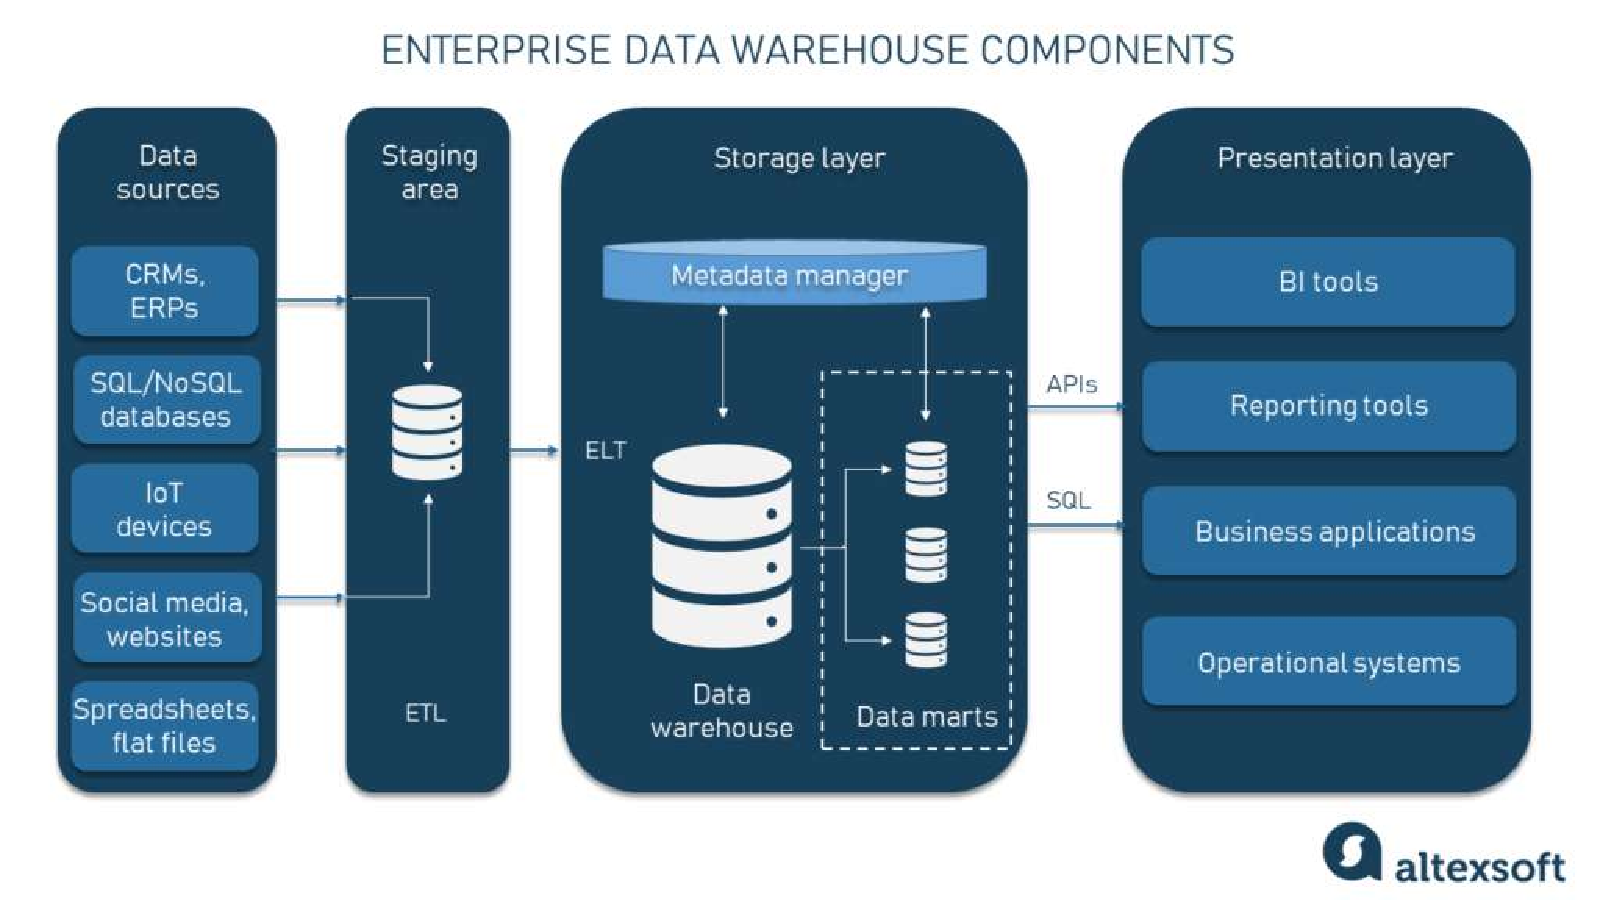
\includegraphics[width=0.8\linewidth]{figure/capitolo_2/Data Warehouse Components.pdf}
    \caption{Componenti di un Data Warehouse}
    \label{fig:Data Warehouse Components}
\end{figure}

\subsection{Architettura dei Data Warehouse}

I data warehouse non sono sistemi semplici. La loro complessità intrinseca, derivata dalla tipologia di problemi che sono destinati a risolvere, ovvero fornire agli analisti una visione unificata e facilmente leggibile delle informazioni, si aggiunge alla mancanza di un preciso modello che permetta di definire quali tecniche o approcci debbano essere applicati e quale sia il metodo per lo sviluppo di tali sistemi \cite{kelly_data_warehousing_in_action}.

Durante gli anni sono state sviluppate diverse architetture per la creazione di un sistema di data warehousing, principalmente possono essere suddivise in tre tipologie \cite{interviewbit_data_warehouse_architecture}:

\begin{itemize}
    \item \textbf{Architetture a singolo livello}. Sono utilizzate per l'elaborazione di dati batch e in tempo reale. I dati vengono prima trasferiti ad un'architettura a singolo livello dove vengono poi convertiti in un formato adatto per l'elaborazione in tempo reale. A questo punto i dati sono trasferiti in un sistema di analisi in tempo reale. Questa architettura è quella più usata poiché la più facile da implementare e poiché la più affine all'elaborazione dei dati operativi. In altre parole, con tale architettura si hanno uno o più database connessi direttamente alle interfacce di analisi che l'utente finale sfrutta per svolgere query di ricerca. L'unica cosa che si frappone tra le interfacce e i database è un middleware per l'elaborazione e la memorizzazione dei dati allo scopo di determinare la qualità dei dati prima che siano adoperati dalle interfacce analitiche.
    \item \textbf{Architetture a doppio livello}. In un'architettura a due livelli il processo analitico è separato da un processo di logica di business, permettendo in questo modo un maggiore livello di controllo ed efficienza. Tale sistema fornisce una migliore comprensione dei dati e permette decisioni più informate. In questa architettura viene aggiunto il livello di data warehouse e ciò permette alla stessa di descrivere un flusso dei dati suddiviso in quattro differenti fasi:
        \begin{enumerate}
            \item \textit{L'origine dei dati} è critica per l'integrità del DW. L'integrità dei dati memorizzati deve essere garantita poiché essa è la rappresentazione del grado di veridicità ed accuratezza dei dati registrati ed un data warehouse deve essere composto di dati che possano essere definiti affidabili.
            \item La \textit{fase di staging dei dati} è un punto chiave del processo ETL e può ridurre significativamente il tempo necessario per la sua esecuzione. L'operazione di ETL è estremamente fondamentale per un processo di data warehousing e per questo motivo migliorare il più possibile tale ambito.
            \item I \textit{metadati} sono un elemento di grande rilevanza in un data warehouse poiché corrispondono alle informazioni che aiutano un amministratore del sistema a decidere le logiche da applicare sulla gestione dei dati. Tali informazioni, permettono di mantenere una coerenza della logica di gestione applicata all'interno del DW, che è un valore critico per una eventuale analisi o report sviluppato su tali dati.
            \item La \textit{profilazione dei dati}\footnote{La \textit{profilazione dei dati} è il processo di esame dei dati disponibili da una fonte di informazioni esistente e la raccolta di statistiche o riepiloghi formativi su tali dati \cite{wikipedia_data_profiling}.} è l'ultimo livello poiché si occupa di convalidare l'integrità dei dati e gli standard di una possibile presentazione. Esso comprende anche analisi avanzate come la generazione di rapporti in tempo reale e batch e le visualizzazioni.
        \end{enumerate}
    \item \textbf{Architetture a triplo livello}. Una architettura a tre livelli aggiunge al livello di origine quello di conciliazione e di data warehouse. Il principale svantaggio del livello di conciliazione è che non sia possibile ignorare completamente i problemi dei dati prima che questi vengano effettivamente conciliati. Più precisamente, il focus principale di chi si occupa di questo compito corrisponde a verificare l'integrità, l'accuratezza e la coerenza dei dati. Ogni volta che si verifica una modifica nei dati, viene eseguito uno strato aggiuntivo di revisione ed analisi di quest'ultimi per garantire che non ne siano stati inseriti nuovi errati. Questa architettura è molto affine a sistemi con un ciclo di vita lungo.
\end{itemize}

%TODO: Sistemare
\begin{comment}  
\begin{figure}[b]
     \centering
     \begin{subfigure}[b]{0.16\textwidth}
         \centering
         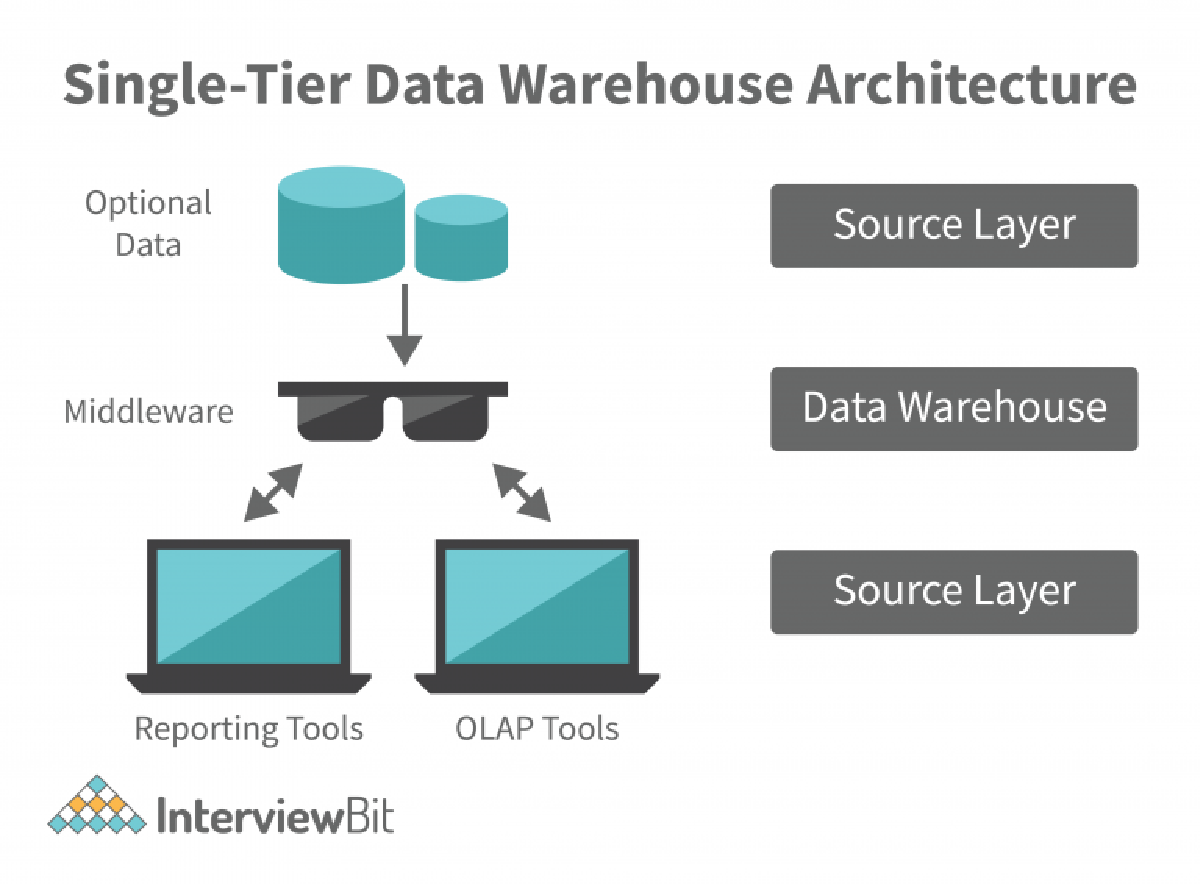
\includegraphics[width=\linewidth]{figure/capitolo_2/DW - Single Tier Architetcure.pdf}
         \caption{Singolo livello}
         \label{DW - Single Tier Architetcure}
     \end{subfigure}
     \hfill
     \begin{subfigure}[b]{0.16\textwidth}
         \centering
         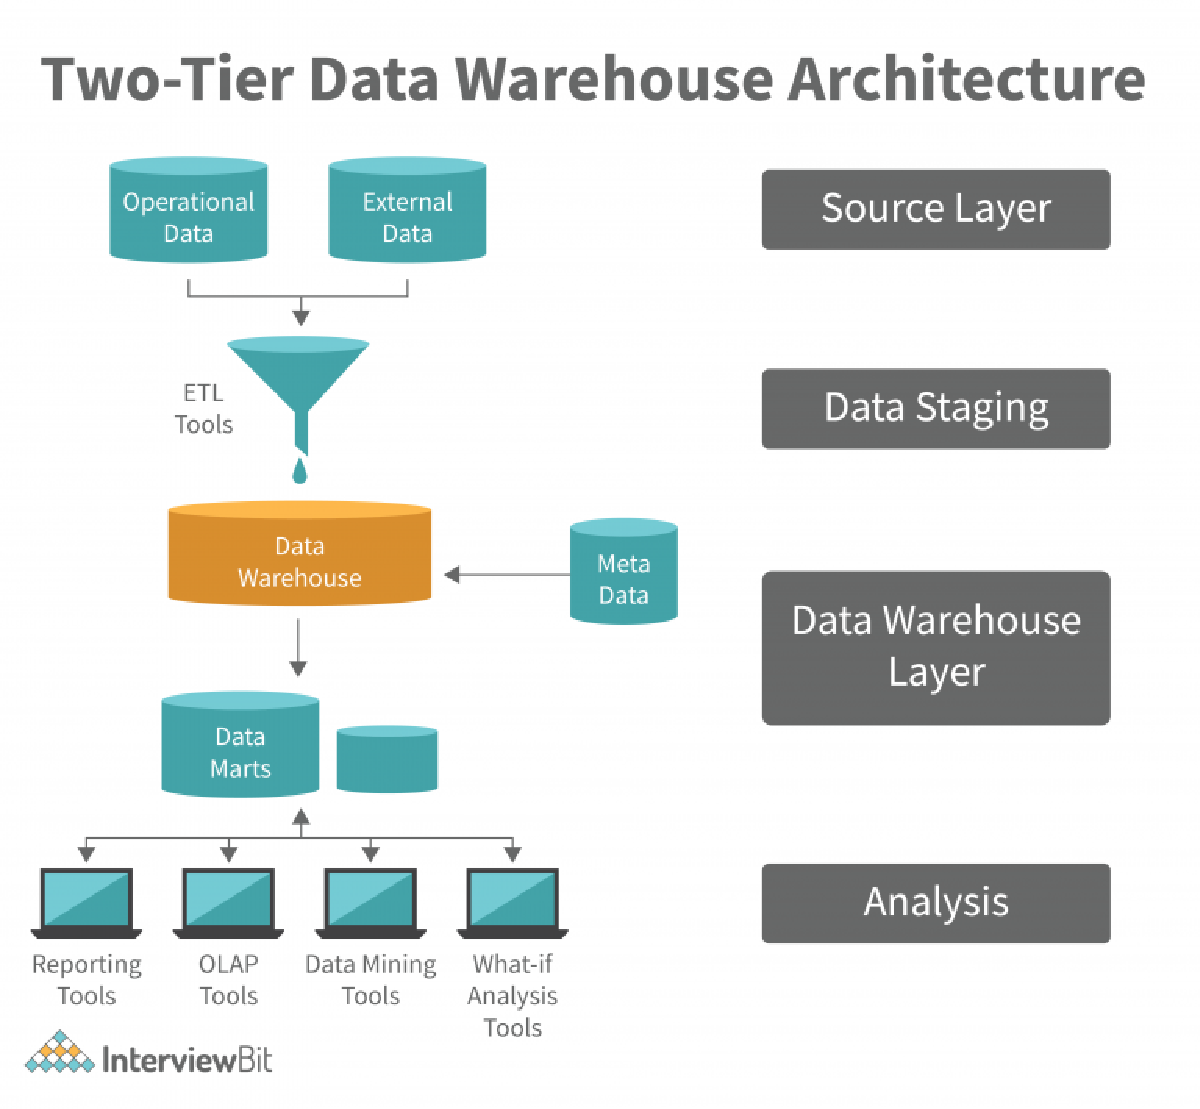
\includegraphics[width=\linewidth]{figure/capitolo_2/DW - Two Tier Architetcure.pdf}
         \caption{Due livelli}
         \label{DW - Two Tier Architetcure}
     \end{subfigure}
     \hfill
     \begin{subfigure}[b]{0.16\textwidth}
         \centering
         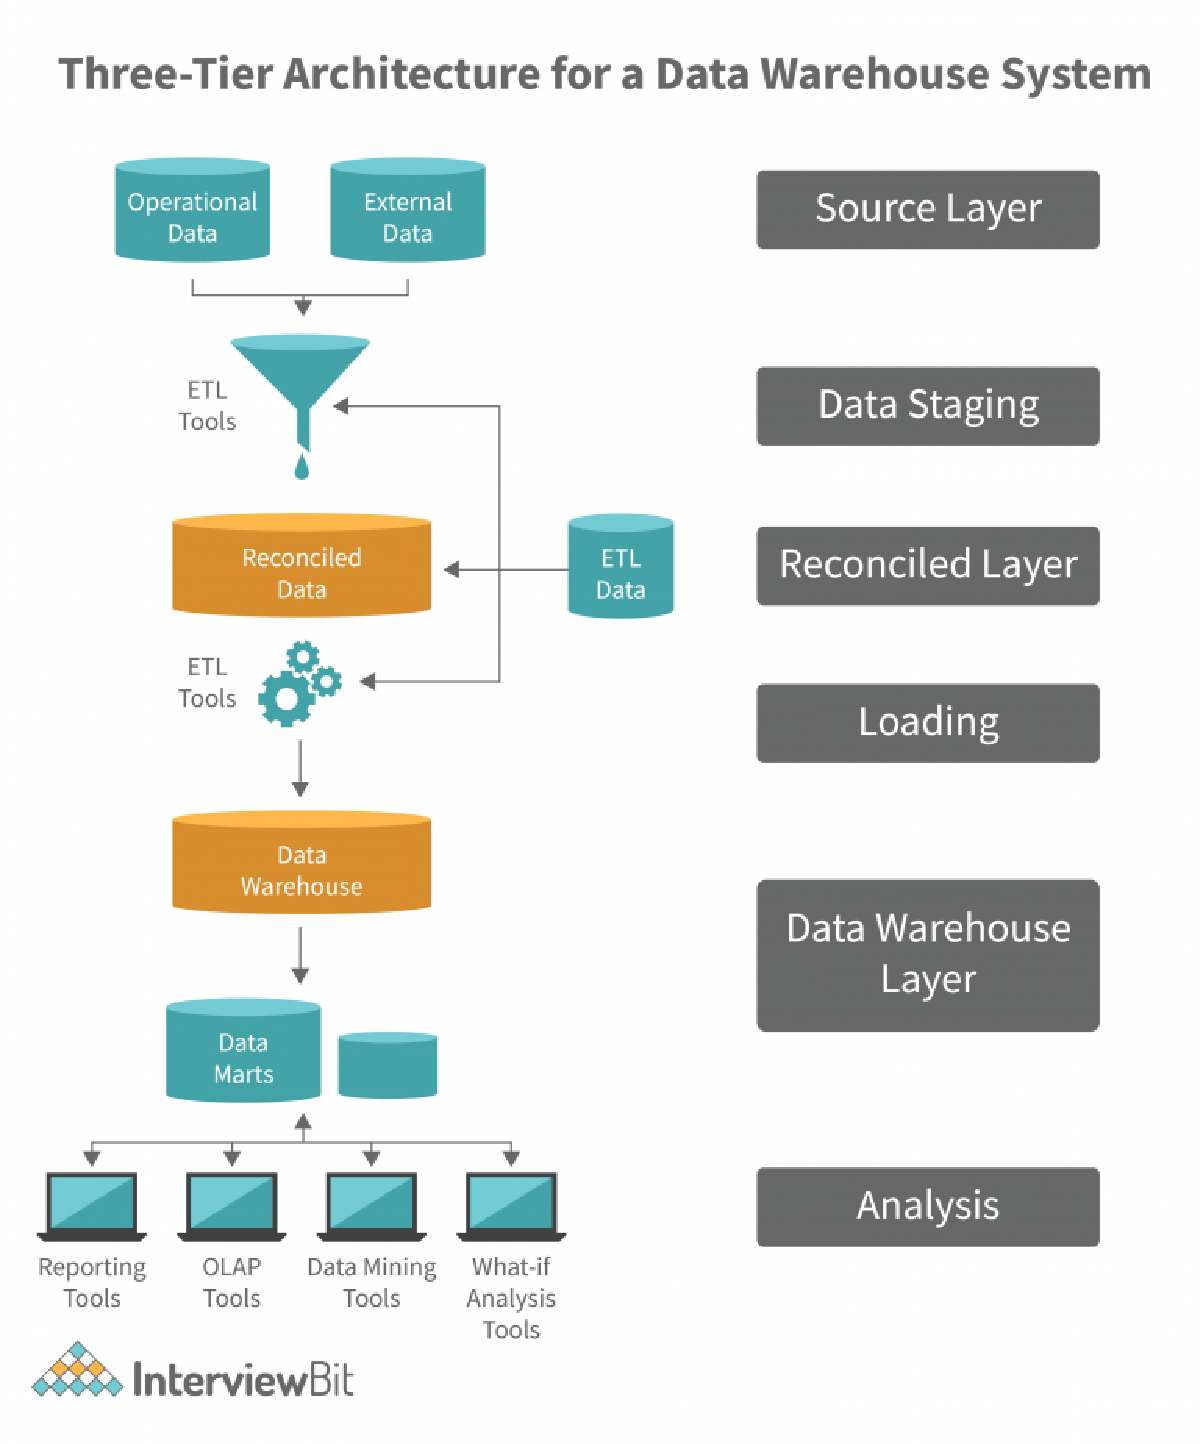
\includegraphics[width=\linewidth]{figure/capitolo_2/DW - Three Tier Architetcure.pdf}
         \caption{Tre livelli}
         \label{fig:DW - Three Tier Architetcure}
     \end{subfigure}
        \caption{Livelli di architetture dei data warehouse}
        \label{fig:data_warehosue_architecture_levels}
\end{figure}
\end{comment}

\subsection{Processo ETL (Extract, Transform, Load)}

In precedenza è stato fatto riferimento alla procedura fondamentale per i data warehouse di raccolta, organizzazione e gestione dei dati dalle varie sorgenti a cui si fa riferimento. Il compito di questa procedura è rendere i dati di un'azienda disponibili recuperandoli da molteplici fonti, ripulire e trasformare tali dati in modo da evitare l'inflazionamento delle informazioni reperibili da eventuali analisi da parte di dati errati o non logicamente corretti. Alcuni esperti del settore hanno indicato che lo sforzo impiegato per questa procedura all'interno di un progetto di data warehousing è pari ad un valore tra il 60\% e l'80\% del totale. Questo perché tale procedura di recupero e gestione dei dati permette di avere informazioni utili/strategiche all'interno del DW. Se questo procedimento non viene fatto correttamente, i dati originari non avrebbero alcuna utilità per la fase di interrogazione ed analisi degli stessi, rendendo l'uso del sistema di data warehousing inutile \cite{researchgate_etl_process}.

Tale procedura si basa su tre operazioni principali, ovvero \cite{sciencedirect_data_warehouse_model}:
\begin{itemize}
    \item \textbf{Estrazione} (\textit{Extract}). Tale operazione è responsabile per il recupero dei dati dai sistemi di origine. Ogni fonte di dati ha un insieme di caratteristiche differenti che devono essere gestite correttamente per permettere un'estrazione efficiente. Per questo motivo, tale fase deve integrare efficacemente sistemi che utilizzano piattaforme, database, sistemi operativi o protocolli diversi tra loro.
    \item \textbf{Trasformazione} (\textit{Transform}). Tale operazione è responsabile di effettuare pulizia ed adattamento (mappatura, trasformazioni, ecc.) dei dati in questione per ottenere dei dati in formati precisi in modo che siano corretti, completi, coerenti e assolutamente non ambigui. Le regole applicate per svolgere ciò dipendono dalle politiche aziendali e da quale tipologia di dati (formati e ambiti trattati) bisogna gestire. Tutte le regole applicate sono descritte nel modulo dei metadati così da poterne tenere traccia.
    \item \textbf{Caricamento} (\textit{Load}). Tale operazione è responsabile del salvataggio dei dati recuperati all'interno del sistema di data warehouse. Naturalmente, essendo molto probabile che la quantità di dati da gestire sia elevata, tale fase deve utilizzare tecniche di ottimizzazione che permettano di aumentare le prestazioni così da permettere agli utenti finali dia vere a disposizione il prima possibile i dati di cui necessitano.
\end{itemize}


\begin{figure}[H]
    \centering
    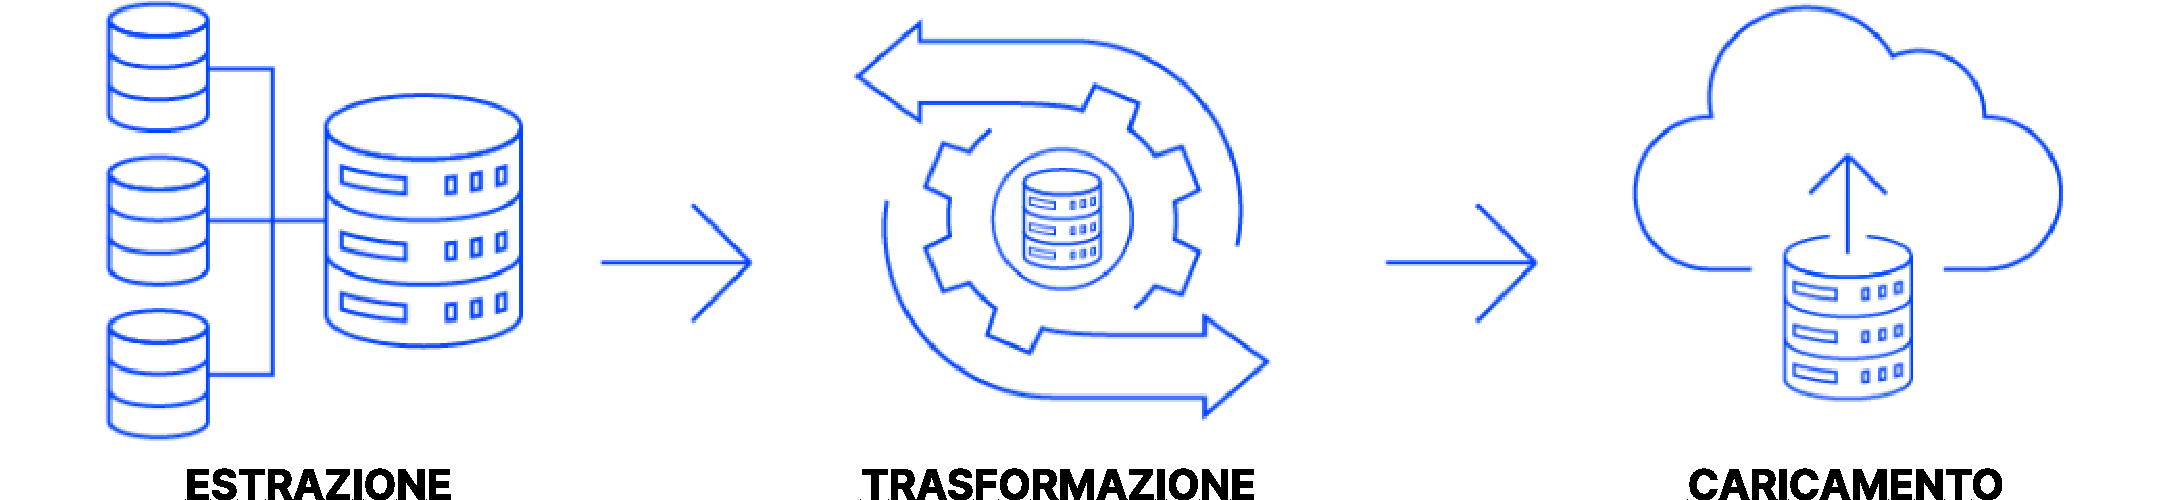
\includegraphics[width=1\linewidth]{figure/capitolo_2/ETL Process.pdf}
    \caption{Processo di ETL}
    \label{fig:ETL Process}
\end{figure}

\subsection{I Metadati}

Nel mondo dei dati, non esistono solo le informazioni essenziali riportate dai dati stessi, ma anche altre informazioni “secondarie” che permettono di descrivere, spiegare, localizzare o contestualizzare le informazioni “principali” dei dati; anche questi sono dei dati, più precisamente prendono il nome di \textit{metadati} (a volte anche definiti grossolanamente come “dati su dati”). Il termine \textbf{metadata} si riferisce alle informazioni che integrano i dati reali. Spesso, i metadati forniscono maggiori dettagli sul contesto del contenuto di un file o danno istruzioni come gestire i dati stessi \cite{ionos_metadata}.

Una volta spiegati cosa sono, è facile comprendere come questi siano una componente importante nel mondo del data warehousing. Una gestione coerente dei metadati permette una riduzione degli sforzi amministrativi e un miglioramento dello sfruttamento del sistema stesso. Una gestione corretta richiede che essi vengano recuperati e memorizzati all'interno di un apposito repository consultabile sia dai vari gruppi di utenti, al fine di essere utilizzato come documentazione da consultare per completare efficientemente i propri compiti, che da prodotti software, come ulteriore risorsa di informazioni e dati da sfruttare per valorizzare i propri lavori. L'esistenza di un singolo repository per la gestione di tutti i tipi di metadati all'interno di un'azienda ne consente una gestione centralizzata, uniforme, coerente e di facile accesso a qualsiasi tipologia di consumatore \cite{metadata_standards}.

\subsection{I Data Mart}

Un \textbf{Data Mart} (\textit{DM}) è archivio dati progettato per contenere dati di uno specifico ambito/argomento. In altre parole, è possibile definire i data mart come delle partizioni del data warehouse complessivo. Essendo una specializzazione di un DW, un DM è meno costoso ed impegnativo in termini di tempi di gestione e ricerca rispetto al sistema totalitario. Pertanto, in generale si può dire che un data mart integra e migliora la funzionalità di un data warehouse più grande.

Come sopracitato i data mart si focalizzano su determinati ambiti o funzionalità, perciò i dati caricati al loro interno che soddisfano tali caratteristiche possono arrivare dallo stesso data warehouse di cui fanno parte, una fonte esterna o altro. In base alla fonte da cui questi dati vengono recuperati è possibile categorizzare un data mart in due modi differenti \cite{itl_data_warehousing_and_mining}:

\begin{itemize}
    \item \textit{Data mart dipendente}. Il data mart è composto recuperando i dati da un data warehouse principale già esistente. Un processo di ETL con un data mart dipendente è semplificato poiché i dati hanno già subito l'operazione di trasformazione per essere caricati nel DW da cui si stanno estraendo. Per questo motivo, il processo di ETL in questo caso è incentrato sull'identificare il sottoinsieme dei dati interessato per il relativo ambiente di richiesta. Questa tipologia è solitamente adoperata per ottenere prestazioni migliori, un controllo più efficiente, maggiore disponibilità e minori costi.
    \item \textit{Data mart indipendente}. Il data mart è composto recuperando i dati da fonti operative, o esterne oppure entrambe. A differenza dei data mart dipendenti, questa tipologia viene creata senza l'uso di un data warehouse principale di riferimento. Tuttavia, in questo caso il processo di ETL non viene semplificato, anzi viene aggravato della necessità di recuperare dati solo di un determinato ambito, complicando la query di ricerca ed estrazione. Questa tipologia ha il vantaggio di essere utile per piccoli gruppi di attività e soddisfa la maggior parte delle esigenze degli utenti ad un costo e tempistiche minori rispetto ad un sistema di data warehouse completo.
\end{itemize}

Di seguito è riportata una tabella riepilogativa che spiega le differenze tra un data mart e un data warehouse:\cite{streamsets_data_mart_vs_data_warehouse}

\begin{comment}
\begin{table}
    \begin{tabular}{ccc}
        Categoria & Data Mart & Data Warehouse\\
        Sorgente dati & Spesso poche fonti di dati, orientate al soggetto e contenenti dati specifici. & Sfruttano molte fonti di dati.\\
        Costi e Grandezza & Entrambi bassi. & Entrambi molto alti.\\
        Performance & Solitamente ha un'alta velocità, dovuta alla quantità limitata di dati. & Potrebbe avere problemi di prestazioni a causa delle loro grandi dimensioni.\\
        Sicurezza & I dati sensibili possono essere omessi completamente. & È necessario adottare misure di sicurezza per proteggere i dati sensibili.\\
        Facilità di implementazione & Può essere abbastanza veloce perché i dati sono pochi. & Potrebbe necessitare di molto tempo, anche anni, data la grande complessità.\\
        Longevità & Solitamente rimossi dopo che lo scopo per il quale sono stati costruiti è stato completato. & Può estendersi per tutta la vita dell'organizzazione.\\
    \end{tabular}
    \caption{Data Mart e Data Warehouse a confronto}
    \label{tab:data_mart_vs_data_warehouse}
\end{table}
\end{comment}

\subsection{I Data Lake}

In precedenza è stato fatto riferimento al termine \textit{data lake}, più precisamente un \textbf{Data Lake} si riferisce a un repository di archiviazione estremamente scalabile contenente una vasta quantità di dati grezzi nel loro formato nativo fino a quando non sia necessario, oltre a sistemi di elaborazione in grado di acquisire dati senza compromettere la struttura dei dati. I data lake sono tipicamente progettati per gestire grandi volumi di dati non strutturati che vengono recuperati rapidamente e da cui vengono estratte ulteriori informazioni. Proprio per questo motivo i data lake adoperano applicazioni di analisi dinamiche, che sappiano adattarsi ai diversi formati di dati archiviati \cite{sciencedirect_data_lake}.

Nella seguente figura \ref{fig:Data Lake Life Cycle} è raffigurato il ciclo di vita dei dati all'interno di un sistema di data lake. Questo schema ad alto livello ci permette di comprendere che mentre i dati confluiscono in determinato punto di acquisizione di un Data Lake, i corrispondenti metadati vengono recuperati e gestiti insieme alla relativa tracciabilità, provenienza e aspetti di sicurezza dei dati, durante il loro ciclo di vita \cite{data_lake_for_enterprices}.

\begin{figure}[H]
    \centering
    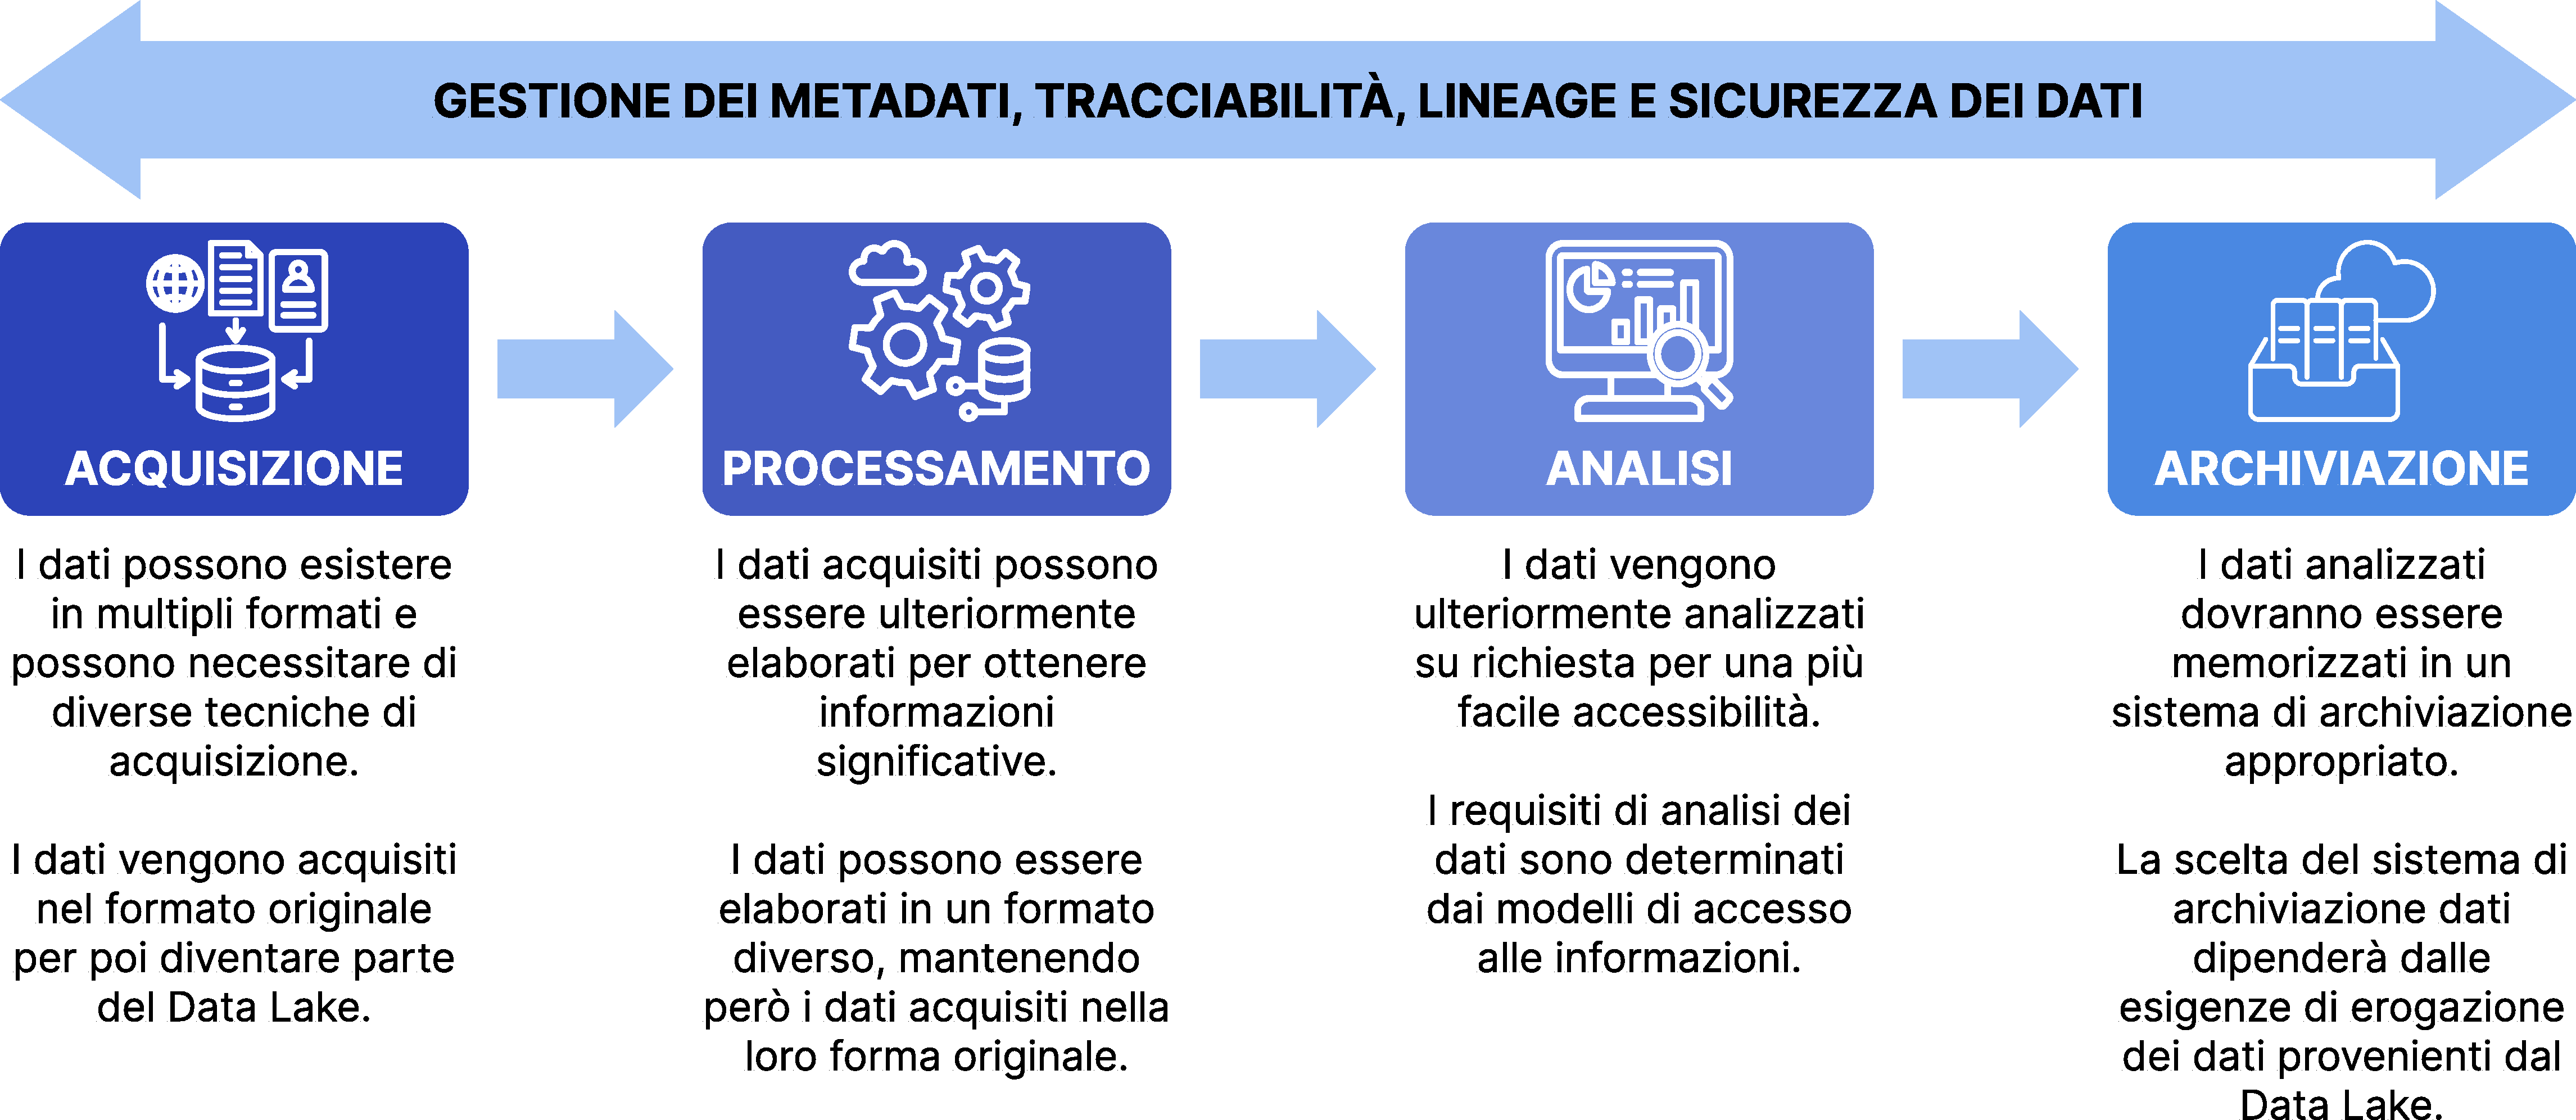
\includegraphics[width=1\linewidth]{figure/capitolo_2/Data Lake Life Cycle.pdf}
    \caption{Ciclo di vita dei dati nei Data Lake}
    \label{fig:Data Lake Life Cycle}
\end{figure}

Originariamente i data lake sono stati creati per sopperire all'incapacità dei data warehouse di gestire i volumi crescenti, la velocità e l'ampia serie di Big Data. I data lake, anche se più lenti dei DW, sono più economici poiché non necessitano delle operazioni di trasformazione. Data la mancanza di necessità di definire degli obiettivi di business da applicare sui dati, hanno tantissimi possibili casi di utilizzo. Tuttavia, i due principali casi di utilizzo comprendono l'esplorazione della data science e le attività di ripristino e backup dei dati \cite{ibm_data_architecture}.

Di seguito è riportata una tabella riepilogativa che spiega le differenze tra un data lake e un data warehouse \cite{aws_data_lake_vs_data_warehouse}.

\begin{comment}
\begin{table}
    \centering
    \begin{tabular}{ccc}
        Caratteristiche & Data Lake & Data Warehouse\\
        Dati & Tutti i dati, compresi strutturati, non strutturati e semi-strutturati. & Dati relazionali da sistemi transazionali, database e applicazioni aziendali.\\
        Schema & Creato al momento dell'analisi. & Spesso progettato prima dell'implementazione, ma può essere creato anche al momento dell'analisi.\\
        Prezzo/Prestazioni & I risultati delle query diventano più veloci utilizzando l'archiviazione a basso costo e il disaccoppiamento dei processi di elaborazione e archiviazione. & Risultati delle query più rapidi utilizzando uno storage locale.\\
        Qualità dei dati & Qualsiasi dato curato e non. & Dati estremamente curati che fungono da versione veritiera centrale.\\
        Utenti & Analisti aziendali, data scientist, sviluppatori ed ingegneri di dati. & Analisti aziendali, data scientist e sviluppatori di dati.\\
        Analisi & Machine learning, analisi esplorativa, rilevamento di dati, streaming, analisi operativa, Big Data e profilazione. & Reporting in batch, BI e visualizzazioni.\\
    \end{tabular}
    \caption{Data Lake e Data Warehouse a confronto}
    \label{tab:data_lake_vs_data_warehouse}
\end{table}
\end{comment}

\subsection{Il Modello Multidimensionale dei Dati}

Secondo diversi studi è emerso che i modelli di dati tradizionali, come il modello E-R e il modello relazionale, non forniscono un buon supporto ai sistemi appositi per la gestione di dati a fini analitici. Per sopperire a tale problematica, nel tempo sono emersi differenti modelli dai dati basati su una visione multidimensionale dei dati in questione. Questi modelli multidimensionali categorizzano i dati come \textit{fatti} (anche definiti come “misure”) o \textit{dimensioni} \cite{ieee_multidimensional_data_modeling}.

Il \textbf{modello multidimensionale} deriva la sua idea dalla constatazione che gli oggetti che influenzano il processo decisionale sono \textit{fatti} che accadono nel mondo aziendale ed ogni occorrenza di un fatto corrisponde ad un evento accaduto. Inoltre, per ognuno dei fatti registrati si è interessati ai valori di insiemi di \textit{misure} o \textit{metriche} che descrivono quantitativamente gli eventi in questione. Poiché gli eventi da registrare sono moltissimi, viene adoperato un modello che permette di selezionarli e raggrupparli come se fossero collocati all'interno di uno spazio n-dimensionale i cui assi, definiti come \textit{dimensioni} di analisi, determinano diverse prospettive per la loro identificazione \cite{unibo_introduzione_al_data_warehousing}.

\subsubsection{Il Cubo Multidimensionale}

I database che sfruttano il modello multidimensionale considerano i dati come cubi che generalizzano i fogli di calcolo a qualsiasi numero di dimensioni. Inoltre, i cubi supportano gerarchie nelle dimensioni e misure senza duplicare le loro definizioni. Una raccolta di cubi correlati costituisce un database multidimensionale oppure un data warehouse. Sebbene l'immagine associabile all'idea del cubo sia di sole tre dimensioni, in realtà un cubo può teoricamente avere un numero indefinito di dimensioni, per quanto l'aumentare di dimensioni comporti la necessità di sistemi appositi per poterli gestire \cite{researchgate_multidimensional_db}.

Più precisamente, in un cubo le dimensioni definiscono la struttura del cubo utilizzata per effettuare le sezioni che lo compongono, mentre le misure forniscono valori numerici aggregati che siano utili all'utente finale. Un cubo consente ad un'applicazione di recuperare i valori delle misure come se queste si trovassero nelle celle del cubo, dove quest'ultime vengono definite per ogni possibile valore riepilogativo. In altre parole, una cella è definita dall'intersezione degli elementi sull'asse delle dimensioni e contiene i valori aggregati delle misure che corrispondono a quella specifica intersezione \cite{microsoft_multidimensional_models}.

\begin{figure}
    \centering
    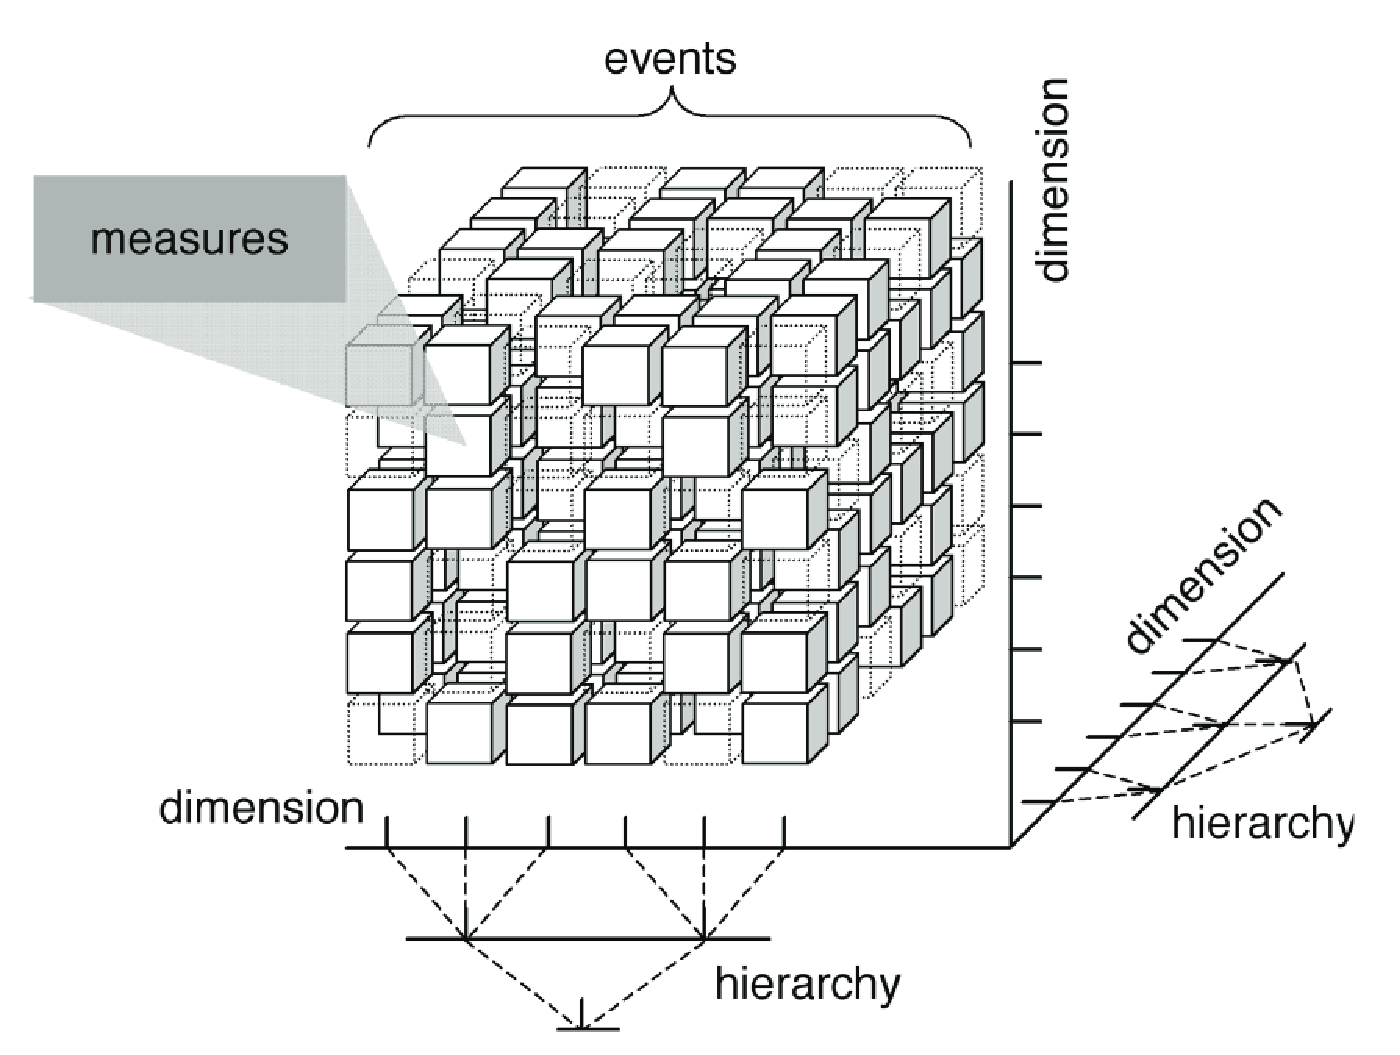
\includegraphics[width=0.85\linewidth]{figure/capitolo_2/Multidimensional Data Cube.pdf}
    \caption{Rappresentazione di dati Multidimensionali sottoforma di cubo}
    \label{fig:Multidimensional Data Cube}
\end{figure}

Per semplificare il concetto, una tabella di un database è strutturata come un foglio di calcolo e memorizza i singoli record in un formato bidimensionale, riga per colonna; ogni fatto corrisponde all'intersezione di due dimensioni, una riga e una colonna. Invece, un cubo multidimensionale estende la singola tabella con livelli ulteriori aggiungendo una dimensione per ogni livello permettendo di rappresentare in questo modo maggiori informazioni per un singolo evento \cite{ibm_multidimensional_data}.

\subsection{Database OLTP e OLAP}

I database relazionali sono stati uno dei punti cardine delle infrastrutture delle applicazioni aziendali per più di venti anni. Con l'avanzare della tecnologia si pose l'obiettivo di fornire alle compagnie un sistema di gestione delle informazioni che coprisse tutti gli ambiti principali che vanno dalla pianificazione dei processi aziendali fino alle analisi individuali; tuttavia, ciò non è stato possibile. Più complessi diventano i requisiti aziendali e maggiore è stato il focus sul migliorare l'elaborazione transazionale, creando appositi database che prendono il nome di sistemi \textbf{OLTP} (\textit{On-Line Transactional Processing}, o "elaborazione transazionale on-line"). Ciò ha comportato la necessità di spostare le applicazioni di ambito analitico e finanziario in sistemi separati ad hoc che avessero maggiore flessibilità e prestazioni, prendendo il nome di sistemi \textbf{OLAP} (\textit{On-Line Analytical Processing}, o "elaborazione analitica on-line"). Entrambi i sistemi sono basati sulla teoria relazionale dei dati, ma utilizzano approcci tecnici differenti. Inoltre, l'OLTP è il prerequisito necessario per l'OLAP, ma solo con l'OLAP le aziende possono comprendere al meglio i dati generati dal proprio lavoro e trarre delle conclusioni che permettano di migliorarlo \cite{scribd_oltp_olap}.

I sistemi OLTP sono strutture progettate per alti volumi di query con accesso specifico con l'obiettivo di massimizzare l'efficienza di queste operazioni, mentre i sistemi OLAP utilizzano tecnologie di archiviazione dei dati per supportare l'analisi e l'estrazione di dati storici a lungo termine per fornire agli analisti dei report da cui ricavare informazioni per prendere decisioni aziendali \cite{ieee_oltp_olap}.
Per comprendere meglio questo discorso, di seguito vengono spiegati i concetti di OLAP e OLTP, in modo da poter approfondire l'argomento.

\begin{itemize}
    \item \textit{OLTP}. Questi database in genere comprendono dati transazionali, ovvero informazioni che tengono traccia delle informazioni correlate alle attività di un'azienda. Gli stati che descrivono le transazioni dei dati devono però essere atomiche\footnote{Un'operazione si definisce \textit{atomica} se questa ha sempre un esito o positivo o negativo, non può rimanere in uno stato parziale.} e coerenti. Tali sistemi sono progettati per elaborare e archiviare in modo efficiente singole transazioni, permettendo in questo modo di gestire grandi quantità di transazioni in modo indipendente \cite{microsoft_oltp}.
    \item \textit{OLAP}. È una tecnologia che consente di organizzare i database aziendali di grandi dimensioni e supporta l'esecuzione di analisi complesse. Può essere usata per seguire query di analisi complesse senza influire negativamente sulle attività dei sistemi transazionali. Poiché i database utilizzati dalle aziende, principalmente OLTP, non sono progettati per sopperire a necessità di analisi, il recupero delle informazioni da questi sistemi è un compito esoso sia in termini di tempo che di prestazioni. A questo scopo sono stati ideati i database OLAP, ottimizzati appositamente per gestire intensi carichi di lavoro in lettura e ridotti in scrittura \cite{microsoft_olap}.
\end{itemize}

Di seguito è riportata una tabella riepilogativa che spiega le differenze tra un database OLAP e uno OLTP \cite{aws_oltp_vs_olap}.

\begin{comment}
\begin{table}
    \centering
    \begin{tabular}{ccc}
        Criteri & OLAP & OLTP\\
        Scopo & Aiuta ad analizzare grandi volumi di dati per supportare il processo decisionale. & Consente di gestire ed elaborare transazioni in tempo reale.\\
        Origine dati & Utilizza dati storici e aggregati provenienti da diverse origini. & Utilizza transazioni in tempo reale provenienti da un'unica origine.\\
        Struttura dei dati & Adopera database multidimensionali (cubi) oppure database relazionali. & Adopera solo database relazioni.\\
        Modello dei dati & Utilizza lo schema a stella, a fiocco di neve oppure altri modelli analitici. & Utilizza modelli normalizzati o denormalizzati.\\
        Volume dei dati & Ha requisiti di archiviazione elevati (TB o PB). & Ha requisiti di archiviazione inferiori (GB).\\
        Tempo di risposta & Ha tempi di risposta più lunghi (s o m). & Tempi di risposta brevi (ms).\\
    \end{tabular}
    \caption{Differenze tra database OLTP e OLAP}
    \label{tab:oltp_vs_olap}
\end{table}
\end{comment}

\section{Analisi dei Dati}

Se il capitolo \ref{ch:Introduzione} ci ha permesso di comprendere quanto i dati siano importanti e come siano diventati tali, con l'attuale sono stati spiegati largamente i concetti di \textit{Big Data}, \textit{Data Warehousing} e \textit{conoscenza} permettendoci di comprendere quali sono le operazioni, le infrastrutture e i modelli necessari alla loro gestione. Tutto ciò si raggruppa in un singolo macro ambito, ovvero quello dell'\textit{analisi dei dati}.

Più precisamente, l'\textbf{analisi dei dati} (o \textit{Data Analytics}) è il processo grazie al quale vengono ricavate le informazioni dai dati, precedentemente estratti, trasformati e centralizzati, per permettere di scoprire, analizzare e comprendere dei possibili schemi (o modelli) nascosti, relazioni, tendenze e anomalie presenti al loro interno. L'obiettivo dell'analisi dei dati è quindi identificare informazioni utili, suggerire conclusioni e aiutare a prendere decisioni accurate \cite{talend_data_analytics}.

\subsection{Tipologie di Analisi}
L'analisi dei dati viene utilizzata per aumentare la produttività e le entrate con una riduzione dei costi in qualsiasi settore. Essa permette di dare un senso a grandi volumi di dati la cui forma grezza è priva di un modello specifico data la loro probabile varietà. Raccogliere e archiviare una quantità così elevata di dati acquisisce valore solamente se ben utilizzati e l'analisi è uno dei migliori modi per farlo \cite{researchgate_big_data_analytics}.
Tuttavia, data l'eterogeneità si dei dati che degli ambiti di utilizzo, è necessario applicare tecniche di analisi differenti dipendentemente dalle proprie necessità. Proprio per questo motivo è possibile suddividere i modelli analitici in quattro tipologie \cite{big_data_analytics_harnessing_data_for_new_business_models}:

\begin{enumerate}
    \item \textbf{Analisi Descrittiva}. Risponde alla domanda “Cosa sta accadendo?”. Corrisponde alla fase preliminare dell'elaborazione dei dati che crea un insieme di dati storici. In altre parole, gestisce ciò che accade in tempo reale e ciò che è accaduto in passato, così da comprendere le cause dei successi e fallimenti avvenuti in passato e conoscere gli eventuali ambiti su cui dover approfondire le proprie conoscenze date le tendenze attuali.
    \item \textbf{Analisi Diagnostica}. Risponde alla domanda “Perché è avvenuto?”. Essa esamina le informazioni passate per conoscere come, cosa e perché un evento è successo. In altre parole, il proprio scopo è quello di scoprire eventuali informazioni che permettano di identificare la causa principale di un problema e quindi i fattori che hanno causato direttamente o indirettamente un avvenimento.
    \item \textbf{Analisi Predittiva}. Risponde alla domanda “Cosa è probabile che accada?”. Questa analisi adopera i dati passati e presenti per prevenire cosa possa accadere in futuro, fornendo le probabilità associate all'evento in questione. Proprio a questo scopo vengono utilizzati sistemi di Data Mining associati a modelli specifici di intelligenza artificiale per svolgere l'analisi e creare i possibili scenari che potrebbero generarsi.
    \item \textbf{Analisi Prescrittiva}. Risponde alla domanda “Cosa si dovrebbe fare?”. Si dedica a riconoscere quale sia l'azione più corretta da intraprendere. Sfruttando i dati prevenienti dalle analisi precedentemente elencate, cerca di trovare la soluzione migliore tra le varie possibili. Essa va oltre la previsione dei risultati futuri, suggerendo anche i benefici dell'azione, secondo le previsioni generate, e mostrando al decisore le implicazioni di ciascuna scelta.
\end{enumerate}

\begin{figure}[H]
    \centering
    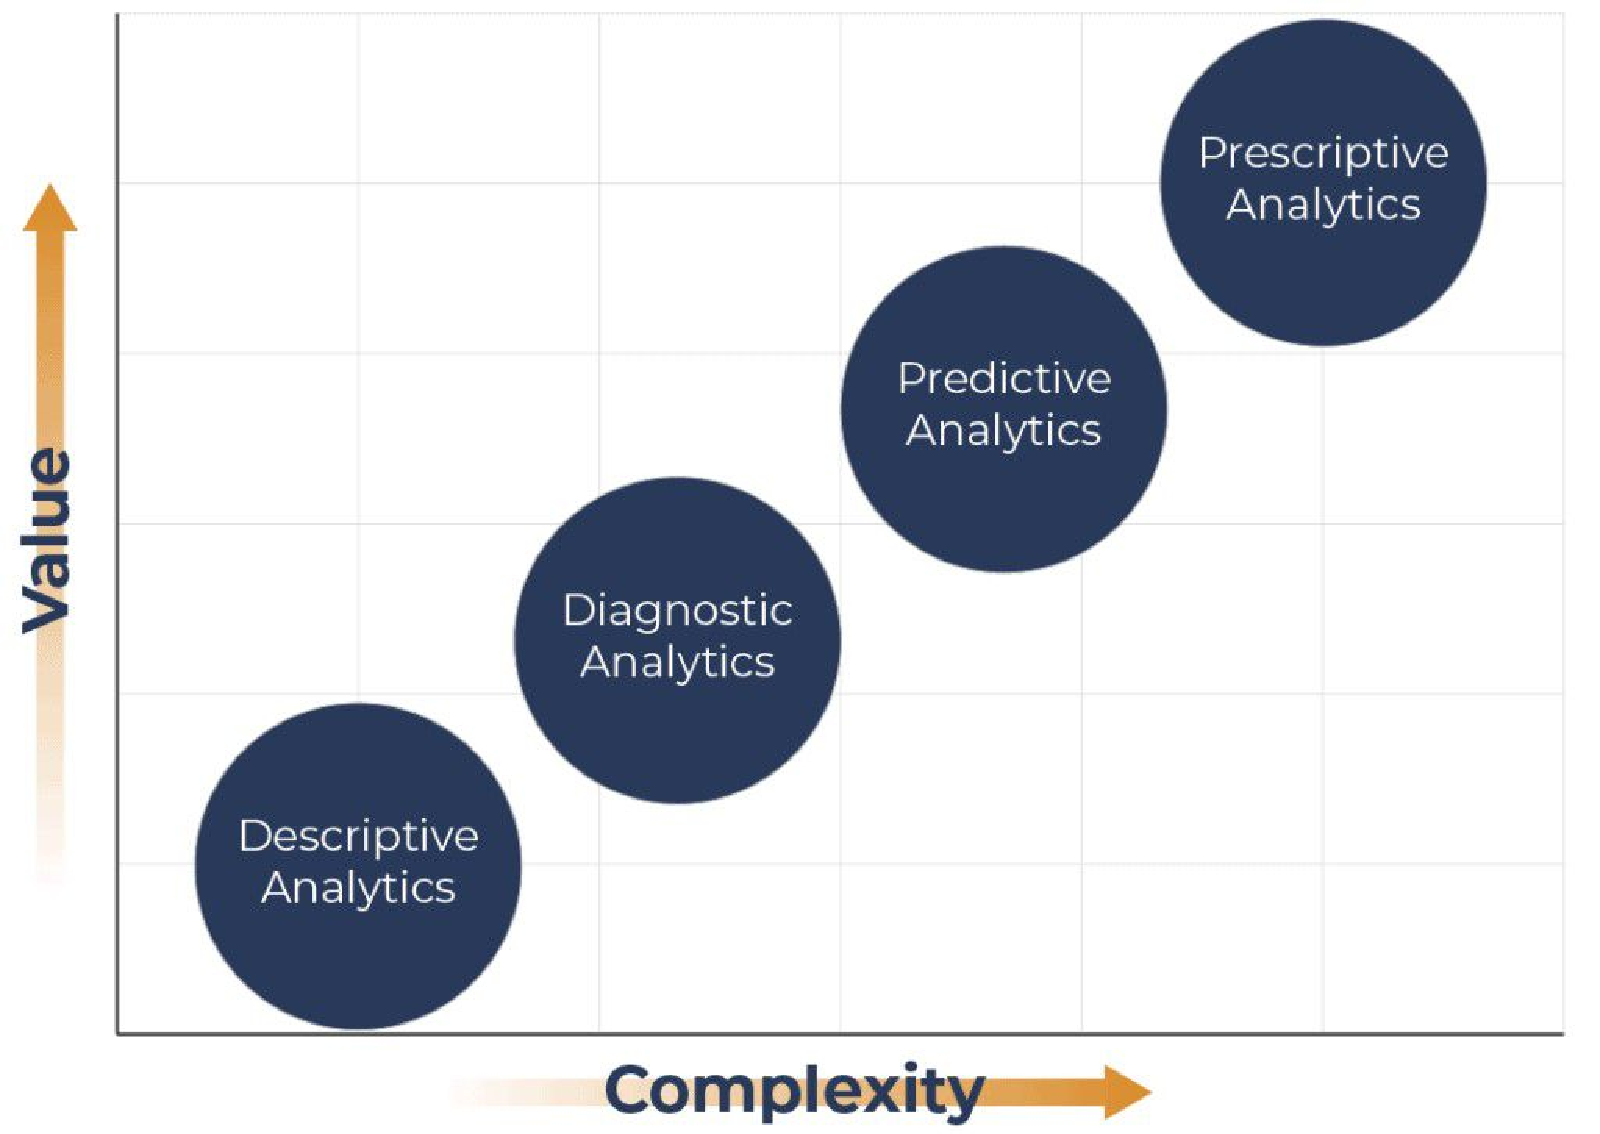
\includegraphics[width=0.75\linewidth]{figure/capitolo_2/Analytics Models.pdf}
    \caption{Tipologie di analisi dei dati}
    \label{fig:Analytics Models}
\end{figure}

\subsection{I Sistemi di Supporto alle Decisioni}

La rapida crescita di dati e quindi il relativo compito di doverli gestire e sfruttare al meglio ha portato ad avere una sempre maggiore necessità di supporto per la comprensione ed analisi degli stessi. Sono stati molti gli studi a riguardo che hanno riscontrato che le soluzioni prodotte dai decision maker sono al di sotto del loro possibile potenziale, poiché essi non sono in grado di assimilare l'elevato numero di informazioni per poter svolgere il proprio compito. Per sopperire a tale problema, sono stati ideati dei \textit{sistemi di supporto alle decisioni}, o \textit{Decision Support Systems} (\textit{DSS}), ovvero strumenti che assistono direttamente i responsabili delle decisioni esecutive nel proprio lavoro semplificando le informazioni da dover sfruttare.\cite{dss_introduction}

La maggior parte delle ricerche sui DSS adotta uno dei seguenti concetti \cite{mit_keen_dss}:

\begin{itemize}
    \item I DSS sono definiti in base alla struttura del compito che devono affrontare.
    \item I DSS richiedono una strategia di progettazione che sia distintiva dipendentemente dalle tecniche di evoluzione e "middle-out".
    \item I DSS supportano i processi cognitivi dei singoli responsabili delle decisioni; la ricerca decisionale fornisce approfondimenti descrittivi sulla risoluzione dei problemi di gestione e teorie normative per definire come migliorarne l'efficacia.
    \item I DSS riflettono una strategia di implementazione per rendere i computer utili ai dirigenti; questa strategia si basa sull'uso di intermediari esperti, servizi reattivi e interfacce software user-friendly.
\end{itemize}

Più precisamente, un \textbf{Decision Support System} è un sistema informativo che aiuta un'azienda nel compito di svolgere attività decisionali che richiedono giudizio, determinazione e una determinata sequenza di azioni. Il DSS assiste la gestione di medio e alto livello dell'azienda che lo adotta analizzando enormi volumi di dati e accumulando informazioni che possono rendersi utili per la risoluzione di problemi o la presa di decisioni \cite{cfi_dss}.

\begin{figure} [H]
    \centering
    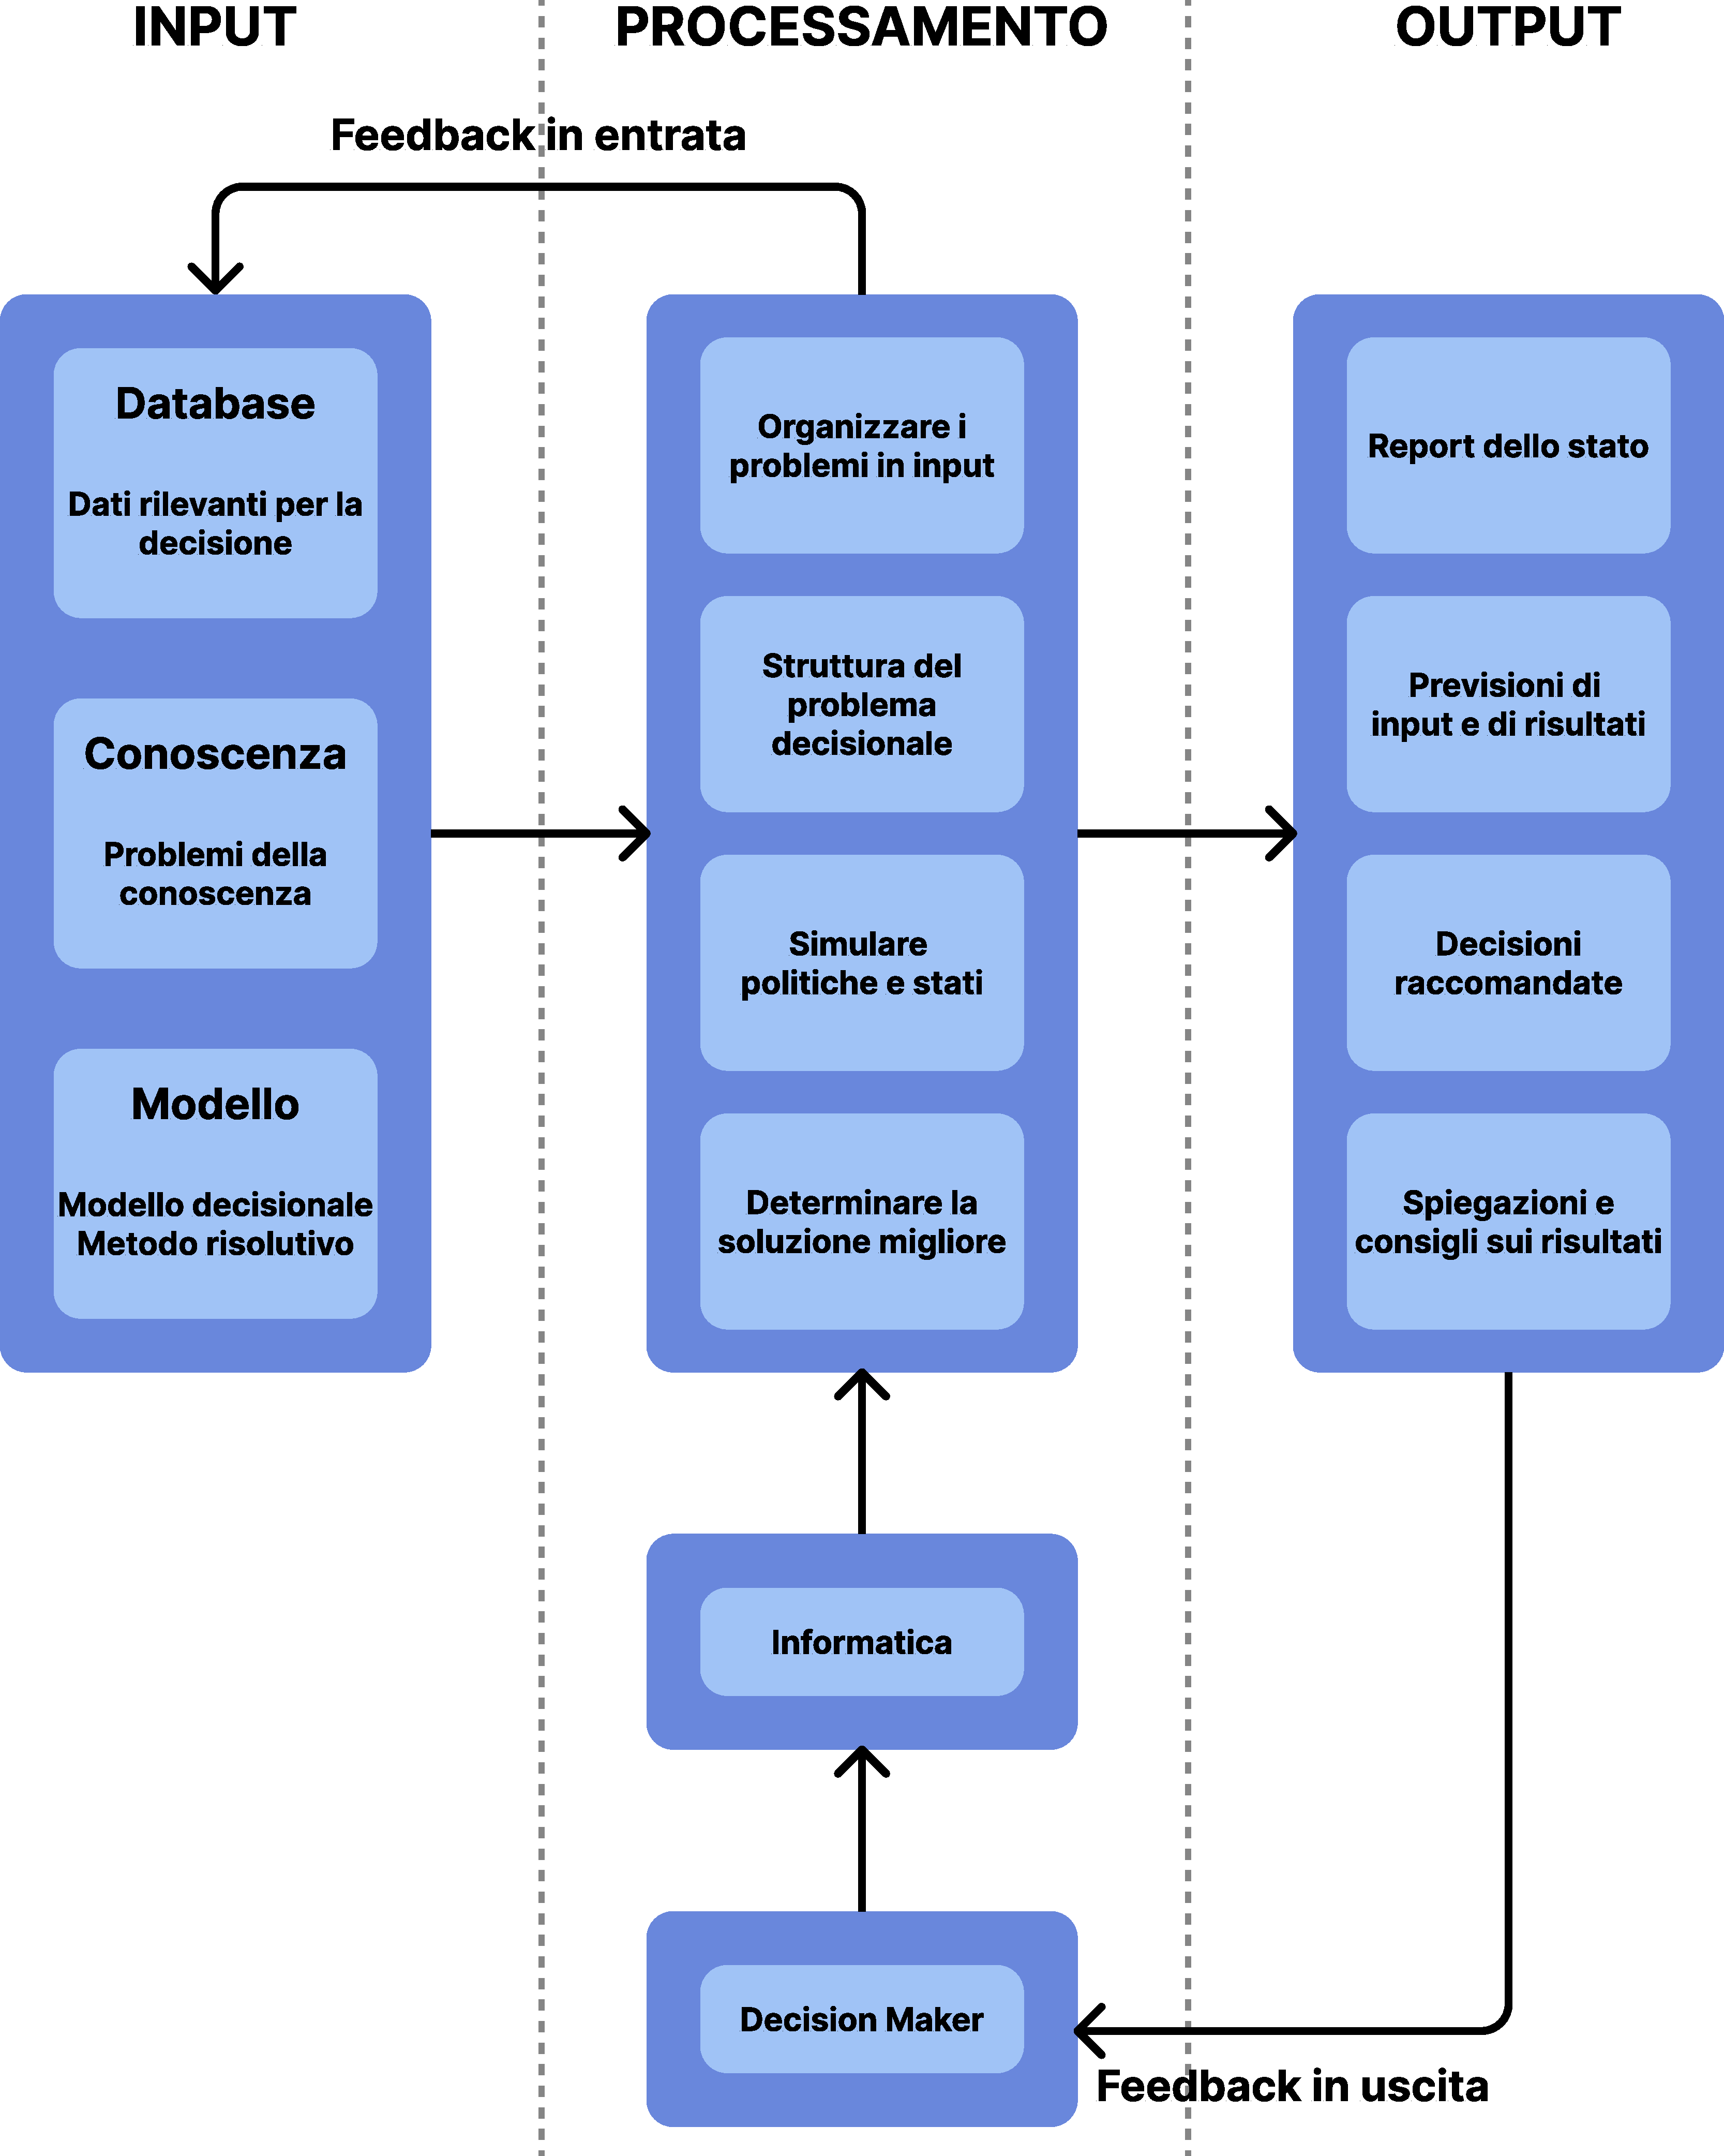
\includegraphics[height=1\linewidth]{figure/capitolo_2/Decision Support System Structure.pdf}
    \caption{Struttura di un sistema decisionale di supporto}
    \label{fig:Decision Support System Structure}
\end{figure}

\subsubsection{Le Caratteristiche}

Identificare le caratteristiche di un sistema decisionale di supporto non è un compito semplice data l'eterogeneità di quest'ultimi e degli ambiti in cui sono adoperati, tuttavia Turban e Aronson sono riusciti a ricapitolare quali siano le caratteristiche generali che li contraddistinguono \cite{dss_characteristics}.

\begin{itemize}
    \item Un DSS assiste i decision maker con la risoluzione di problemi semi e non strutturati facendo uso del giudizio umano e dei computer.
    \item Un DSS copre un ampio spettro di livello di gestione, dal mondo dirigenziale a quello operativo.
    \item Un DSS fornisce supporto indifferente ad individui singoli o gruppi.
    \item Un DSS facilita la presa di decisioni indipendenti e/o sequenziali che possono essere prese una o più volte.
    \item Un DSS gestisce tutte le fasi del processo decisionale, ovvero: raccolta di informazioni, progettazione, scelta ed implementazione.
    \item Un DSS copre un'ampia varietà di strumenti di analisi delle decisioni.
    \item Un DSS è adattabile e flessibile, permettendo agli utenti di aggiungere, modificare, eliminare o riorganizzare gli elementi base di cui si compone.
    \item Un DSS dovrebbe essere user-friendly.
    \item Un DSS ha l'obiettivo di migliorare l'efficacia della presa di decisioni (appropriatezza e qualità) anziché l'efficienza (il costo della presa di decisioni).
    \item Un DSS deve assistere e non sostituire un decision maker.
    \item Un DSS adotta diversi modelli di analisi per creare strategie diverse dipendentemente dalla situazione in cui si riscontra il problema.
    \item Un DSS dovrebbe essere in grado di fornire accesso a una varietà di fonti e formati differenti di dati.
    \item Un DSS può essere integrato con altri sistemi e può essere distribuito tramite tecnologie di rete e web per essere facilmente fruibile.
\end{itemize}

\subsubsection{Tipologie di DSS}

I sistemi di supporto alle decisioni possono essere suddivisi in differenti categorie dipendentemente dal principio su cui si basano, ovvero \cite{techtarget_dss_types}:

\begin{itemize}
    \item \textit{Basati sui dati}. Questa tipologia basa il proprio supporto sui dati provenienti da database (interni o esterni) sfruttando principi di data mining per poterli analizzare e mostrare all'utente.
    \item \textit{Basati sui modelli}. Questa tipologia basa il proprio supporto sull'analizzare una situazione che corrisponda ad un modello/schema precedentemente definito in base ai requisiti dell'utente.
    \item \textit{Basati sulla comunicazione e DSS di gruppo}. Questa tipologia basa il proprio supporto sull'adottare diversi strumenti di comunicazione per consentire a più di una persona di lavorare su una specifica attività, con l'obiettivo di migliorare il valore delle scelte dovute ad una collaborazione tra più persone.
    \item \textit{Basati sulla conoscenza}. Questa tipologia basa il proprio supporto sull'utilizzo di una conoscenza aggiornata continuamente e gestita da un sistema di \textit{Knowledge Mangament} in modo da fornire informazioni sempre aggiornate e coerenti basate sulla conoscenza generale dell'azienda.
    \item \textit{Basati sui documenti}. Questa tipologia basa il proprio supporto sull'analisi dei documenti (interni o esterni) per rispondere a ricerche specifiche degli utenti e fornirgli le informazioni necessarie. 
\end{itemize}


\subsection{Business Intelligence (BI) e Business Analytics (BA)}
Come detto in precedenza, l'analisi dei dati è un termine ampio utilizzato per comprendere diverse metodologie di analisi dei dati. Tra queste metodologie due delle più rilevanti in ambito aziendale sono sicuramente la \textit{Business Intelligence} (\textit{BI}) e la \textit{Business Analytics} (\textit{BA}) (che inoltre, possono essere identificati anche come dei sistemi di supporto alle decisioni).

In termini generici, la BI e la BA si riferiscono all'infrastruttura collettiva, agli strumenti, alle applicazioni e ad altre risorse che generano dati e informazioni, che a loro volta valorizzano il modo in cui le aziende prendono decisioni, scoprono opportunità di guadagno e esaminano le proprie prestazioni \cite{hpe_bi_and_a}.

Di seguito sono riportate delle spiegazioni generali per comprenderle meglio \cite{academiaedu_bi_and_ba}.

\begin{itemize}
    \item \textit{Business Intelligence}. La BI può essere descritta come un insieme di tecniche e strumenti che permettono l'acquisizione e la trasformazione di dati grezzi in informazioni importanti ed utili per fini aziendali. Tali tecniche sono in grado di gestire enormi quantità di dati (strutturati e in alcuni casi anche non) per permettere l'identificazione, lo sviluppo e la creazione di nuove opportunità strategiche utili alla compagnia.
    \item \textit{Business Analytics}. La BA può essere descritta come l'insieme di competenze, tecnologie e pratiche atte all'esplorazione continua e iterativa delle prestazioni passate di una compagnia al fine di ricavare possibili intuizioni ed aiutare quindi la pianificazione delle decisioni aziendali sulle future azioni da intraprendere. Tali tecniche si concentrano sullo sviluppo di nuove intuizioni e sulla comprensione delle prestazioni aziendali passate basandosi su dati e metodi statistici, in modo da migliorarne le future.
\end{itemize}

\begin{figure}[H]
    \centering
    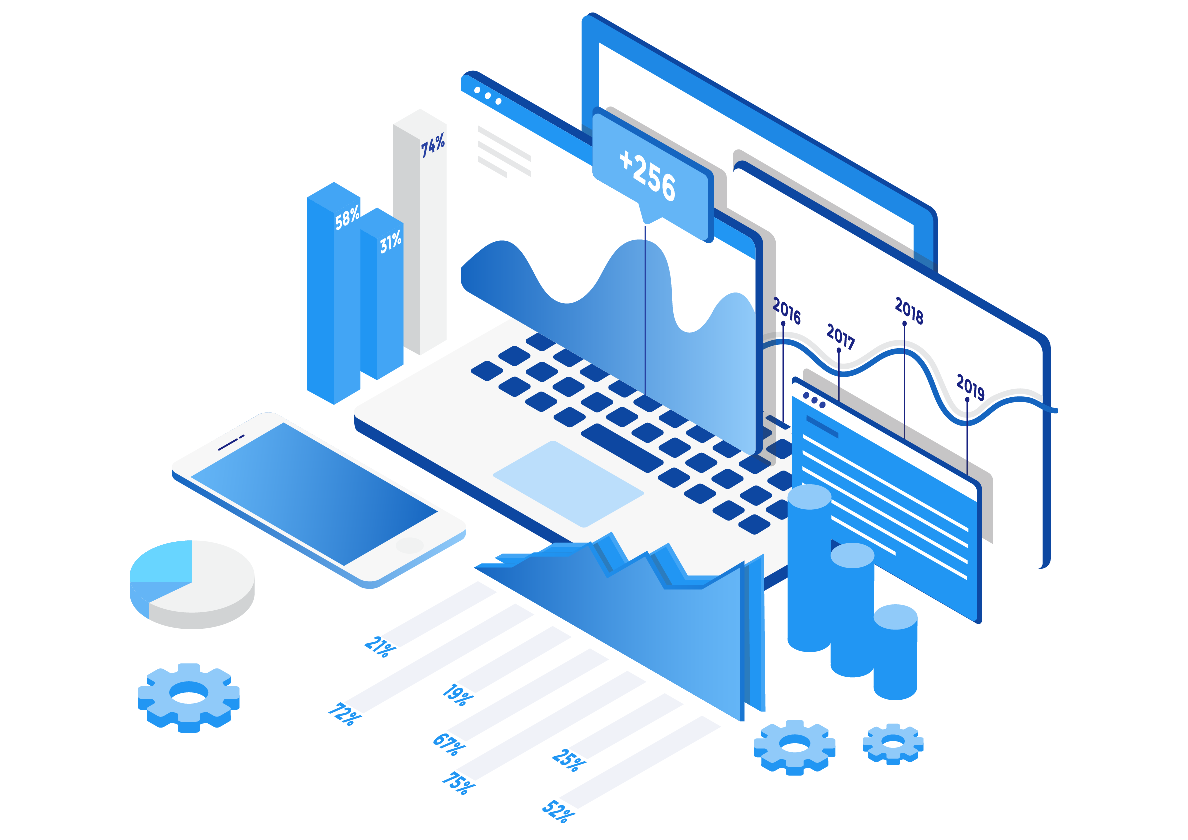
\includegraphics[width=0.75\linewidth]{figure/capitolo_2/Business Intelligence - Business Analytics.pdf}
    \caption{Business Intelligence/Analytics}
    \label{fig:Business Intelligence - Business Analytics}
\end{figure}
\chapter{La Business Intelligence e la Business Analytics}
\label{ch:Business Intelligence and Analytics}

Come spiegato in precedenza, l'analisi dei dati è un termine "astratto" utilizzato per fare riferimento ad un processo di multiple azioni atte a gestire i dati e ricavarne informazioni. Di quest'ultima parte solitamente se ne occupa il mondo della business intelligence e della business analytics. Questi processi solitamente si interfacciano direttamente con il sistema di data warehouse predisposto dall'azienda (entrando in questo modo nel \textit{livello di presentazione} dello stesso).  

\section{La Business Intelligence}
In generale il termine Business Intelligence viene utilizzato per indicare \cite{meauserement_of_bi}:

\begin{itemize}
    \item Informazioni e conoscenze rilevanti che descrivono l'ambiente aziendale, l'organizzazione stessa e la sua situazione in relazione ai mercati, ai clienti, ai concorrenti e alle questioni economiche.
    \item Un processo organizzato e sistematico attraverso il quale le organizzazioni acquisiscono, analizzano e diffondono informazioni da fonti interne ed esterne significative per le loro attività commerciali e per il processo decisionale.
\end{itemize}

Più precisamente, la \textbf{Business Intelligence} (\textbf{BI}) si può definire come «un approccio attivo, basato su modelli e prospettico per scoprire e spiegare aspetti nascosti e rilevanti per le decisioni in grandi quantità di dati aziendali per informare meglio i processi decisionali aziendali» \cite{bi_strategic_intelligence}.

\begin{figure}[!h]
    \centering
    
\includegraphics[width=0.75\linewidth]{figure//capitolo_3/Business Intelligence.pdf}
    \caption{La Business Intelligence}
    \label{fig:Business Intelligence}
\end{figure}

Come abbiamo potuto vedere in precedenza, per i processi di analisi e gestione dei dati non esistono delle definizioni fisse che indichino quali processi, protocolli, modelli o infrastrutture siano necessari per poterli svolgere. In un mondo in cui la tecnologia è in continua evoluzione tali elementi cambiano con essa, differenziando inoltre da azienda ad azienda e da business a business a seconda delle situazioni e necessità. Per questo motivo si può generalizzare il concetto dicendo che «la business intelligence è essenzialmente una conoscenza del business tempestiva, accurata, di alto valore e perseguibile, nonché i processi di lavoro e le tecnologie utilizzate per ottenerla» \cite{bi_for_dummies}.

Quindi, la BI è identificabile come il risultato finale e naturale dell'unione di diversi sistemi e processi, definiti precedentemente, atti a supportare il processo decisionale di un'azienda. L'emergere dell'uso di sistemi di data warehousing, i progressi svolti nella pulizia dei dati, le maggiori capacità di hardware e software e l'evoluzione delle tecnologie connesse ad Internet si combinano per creare un ambiente ricco ed utile per la business intelligence. Principalmente, la BI attinge informazioni da differenti sistemi \cite{researchgate_bi_systems}.

\begin{figure}[!h]
    \centering
    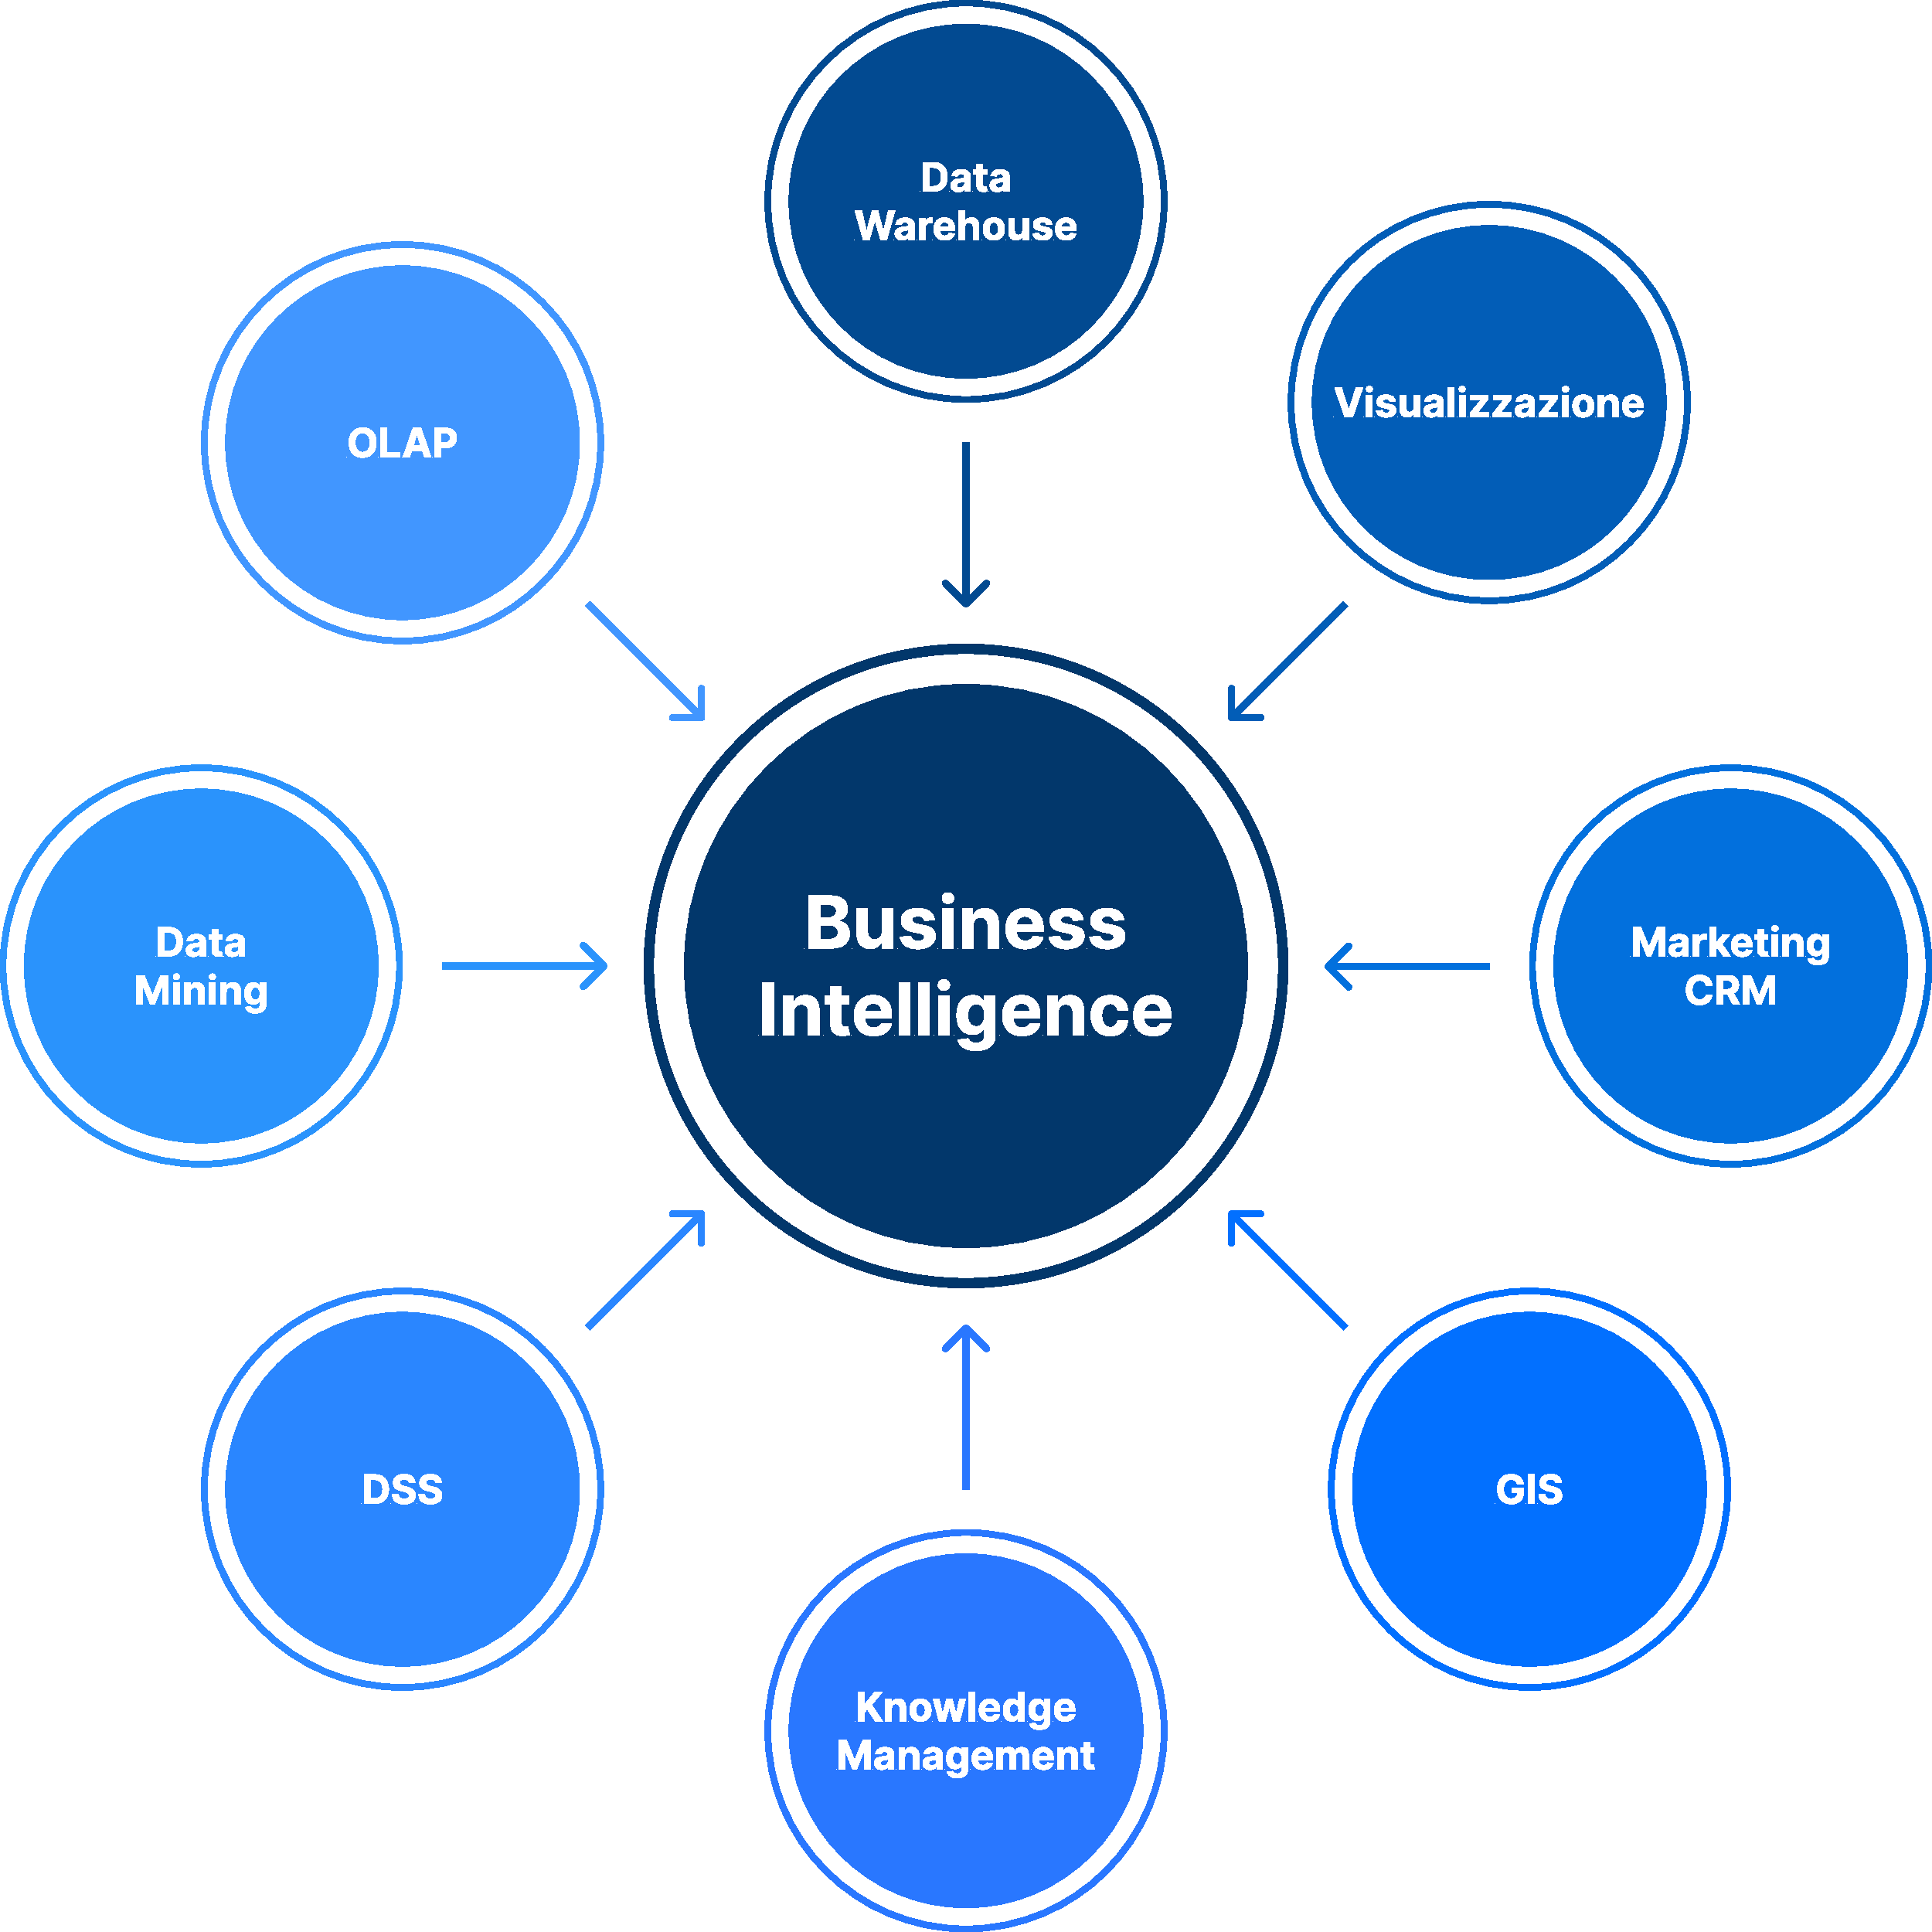
\includegraphics[width=0.8\linewidth]{figure//capitolo_3/Business Intelligence Systems.pdf}
    \caption{Sistemi di integrazione con la Business Intelligence}
    \label{fig:Business Intelligence Systems}
\end{figure}

\subsection{L'apporto della Business Intelligence}

\subsubsection{Il valore}

Dal punto di vista economico, il valore aziendale di un investimento è misurato come il valore attuale netto dei flussi di cassa dopo le imposte associate all'investimento in questione.\footnote{\textit{Il flusso di cassa al netto delle tasse} (\textit{CFAT}) è una misura della performance finanziaria che mostra la capacità di un'azienda di generare flussi di cassa (ovvero, la liquidità netta e gli equivalenti liquidi trasferiti dentro e fuori da un'azienda) attraverso le sue operazioni \cite{cfat_definition}}.
Allo stesso modo, un investimento nell'abito della Business Intelligence crea un bene che deve essere adoperato per generare CFAT incrementali, per far si che comporti aumento delle entrate, riduzione dei costi o entrambi. In altre parole, il valore aziendale della BI risiede nel suo utilizzo all'interno dei processi di gestione che influenzano i processi operativi che generano entrate o riducono costi, e/o nel suo utilizzo all'interno degli stessi processi operativi che lo adottano \cite{decisionpath_bi_value}.

\subsubsection{I benefici}

Nella gestione aziendale un efficiente accesso ai dati può costituire uno strumento di business in grado di migliorare l'efficacia dei processi decisionali, grazie soprattutto alla individuazione delle informazioni necessarie a perseguire uno dei principi che costituiscono il punto di forza per eccellenza, ovvero il miglioramento continuo. Nell'ottica di un costante processo di miglioramento può essere determinante l'individuazione dei possibili punti di forza e/o di debolezza del core business, oltre all'individuazione delle opportunità e delle vulnerabilità, definendo le linee guida e le istruzioni operative che solo da una analisi approfondita possono scaturire, grazie anche ad un approccio derivante da una pianificazione strategica aziendale consapevole \cite{dalla_bi_al_dw}.

Per questo motivo, le aziende hanno iniziato ad adoperare sistemi di Business Intelligence nei propri processi decisionali. Per comprendere meglio a cosa sia dovuto questo alto valore di ROI\footnote{Il \textit{Return Of Investment} (\textit{ROI}, o \textit{ritorno sull'investimento}) è una misura di performance utilizzata per valutare l'efficienza o la redditività di un investimento misurando direttamente l'ammontare del rendimento di un particolare investimento rispetto al suo costo \cite{investopedia_roi}.} di seguito sono riportati tutti i vantaggi ricavabili dall'uso della BI nella propria azienda \cite{oracle_business_intelligence}.

\begin{itemize}
    \item Migliorare l'accuratezza dei dati.
    \item Prendere decisioni migliori più rapidamente.
    \item Migliorare i risultati mission-critical.
    \item Condividere i dati tra aree funzionali aziendali.
    \item Ottenere una maggiore visibilità delle informazioni finanziarie e operative.
    \item Identificare e ridurre le inefficienze.
    \item Eliminare sprechi, frodi e abusi.
    \item Migliora la produttività e il morale dei lavoratori.
    \item Aumentare il ritorno sull'investimento riducendo il costo totale di proprietà.
    \item Migliorare la trasparenza e il servizio a tutti i livelli.
\end{itemize}

\subsubsection{I punti chiave che indicano la necessità di BI}

Di seguito sono riportati otto punti chiave che indicano la necessità da parte di un'azienda dell'adozione di una soluzione di Business Intellingence per migliorare la propria gestione \cite{boomper_book_of_bi}.

\begin{itemize}
    \item \textit{Difficoltà nell'accesso ai dati}. In settori competitivi, è essenziale che le aziende possano accedere rapidamente ai propri dati. Di conseguenza, è essenziale che i decision maker accedano a specifiche informazioni con facilità e immediatezza.
    \item \textit{Dati provenienti da diverse fonti}. Quando un'azienda raccoglie dati da varie fonti, consolidarli in informazioni utili può essere difficile (diversi dipartimenti possono adottare metodologie o formati differenti per il salvataggio e il reporting dei dati). La BI può contribuire a unificare questi dati.
    \item \textit{Dipendenza dai fogli di calcolo}. Utilizzare i fogli di calcolo come principale mezzo per archiviare le informazioni con l'aumentare dei volumi di dati e della loro complessità è un processo inefficiente, tedioso e complicato. Una soluzione di BI può contribuire a razionalizzare il processo di raccolta, analisi e reportistica dei dati.
    \item \textit{Blocchi nella reportistica}. In molte aziende, la business intelligence e la reportistica sono completamente di competenza del reparto \textit{IT}\footnote{Il termine \textit{IT} fa riferimento all'intero spettro di tecnologie per l'elaborazione delle informazioni (compresi software, hardware, tecnologie di comunicazione e servizi correlati). Generalmente, l'ambito dell'IT non include tecnologie integrate che non generano dati per uso aziendale.\cite{gartner_it}}. Ciò può creare blocchi nel processo di reportistica e ritardi che possono rendere obsolete le informazioni. Una soluzione di BI può contribuire a ridurre questi blocchi dando più potere alle persone attraverso la capacità di autogestire e creare i propri report senza la necessità di conoscenze o esperienza tecniche.
    \item \textit{I tuoi dati non forniscono insight attuabili}. Le aziende possono spesso focalizzarsi così tanto sul processo di raccolta dati che finiscono col trascurare l'importanza della produzione di \textit{insight}\footnote{Le \textit{insight}, o \textit{intuizioni}, sui dati sono le conoscenze che un'azienda ottiene analizzando insiemi di informazioni relative a un determinato argomento o situazione, fornendo in questo modo spunti che aiutano le aziende a prendere decisioni \cite{datarobot_insight}.} applicabili. Per questo motivo le aziende dovrebbero adottare un approccio basato sulla qualità piuttosto che sulla quantità dei dati (evitando di raccogliere semplicemente grandi quantità di informazioni prive di significato).
    \item \textit{Dati obsoleti}. Uno dei principali problemi che affligge le aziende è che i loro dati non sono aggiornati. Ciò potrebbe dipendere da ritardi nella raccolta, analisi o reportistica delle informazioni e può avere conseguenze negative sulle prestazioni aziendali. Una soluzione di BI può automatizzare l'elaborazione e la consegna dei dati, con molte soluzioni in grado di pianificare i report in anticipo, garantendo che i dirigenti aziendali dispongano sempre delle informazioni necessarie.
    \item \textit{Difficoltà nella visualizzazione dei dati}. La visualizzazione dei dati è una parte fondamentale della Business Intelligence, ma senza l'esistenza di una soluzione di BI, spesso viene trascurata. I dati una volta raccolti andrebbero sfruttati per essere definibili come utili.
    \item \textit{Impossibilità di accedere ai dati su dispositivi multipli}. Al giorno d'oggi, è sempre più importante che le informazioni siano accessibili in qualunque momento e luogo. Per questo motivo nuovi strumenti di BI sono indirizzati verso un approccio che permetta di utilizzarli da dispositivi multipli.
\end{itemize}

\subsection{Sviluppo di una soluzione aziendale}

\subsubsection{Processo ciclico}
Un processo di Business Intelligence, per quanto possa differire per approccio, l'argomento e lo scopo di riferimento, in generale è caratterizzato da alcuni passaggi fondamentali per la sua implementazione, ovvero \cite{citeseerx_bi_process}:

\begin{enumerate}
    \item \textit{Analisi}. Prima di essere predisposto per l'utilizzo, è necessario svolgere un'analisi dei requisiti che indichi quali sono i KPI\footnote{Un indicatore chiave di prestazioni (\textit{Key Performance Indicator}, o \textit{KPI}) si riferisce ad una misurazione quantificabile utilizzata per valutare le prestazioni a lungo termine di un'azienda rispetto a quello specifico ambito di interesse, aiutando a determinare i risultati strategici, finanziari e operativi di una compagnia (potendo anche metterli a paragone con altri competitor dello stesso settore).\cite{investopedia_kpi}} richiesti dagli utenti finali. Tale fase permette di identificare, ad alto livello,i vari componenti che una possibile soluzione dovrebbe integrare.
    \item \textit{Progettazione}. Sulla base dei requisiti stilati nella fase precedente, in questa vengono identificate specificatamente quali tecnologie siano appropriate per rendere reale la soluzione precedentemente ideata.
    \item \textit{Sviluppo}. Questa fase comporta la messa in atto di tutti i processi studiati, delle infrastrutture progettate e dei modelli di analisi scelti. L'implementazione, inoltre, dipende spesso anche dalla tipologia di dati che dovranno essere gestiti dal sistema, poiché ognuno può necessitare di funzionalità differenti.
    \item \textit{Distribuzione}. Una volta implementata e testata, la soluzione viene messa a disposizione degli utenti finali. Sono proprio quest'ultimi le persone da cui dipende la riuscita finale del progetto, poiché tale fase include lo sviluppo di report e analisi predefinite per i decision maker aziendali.
    \item \textit{Evoluzione}. Tale fase si può dire che è ciò che rende ciclico l'intero processo appena esplicato. Questo perché bisogna sempre valutare il successo del sistema creato per poi estenderlo con ulteriori funzionalità e anche modificare, ottimizzare e rivalutare scelte fatte in precedenza.
\end{enumerate}

\begin{figure} [H]
    \centering
    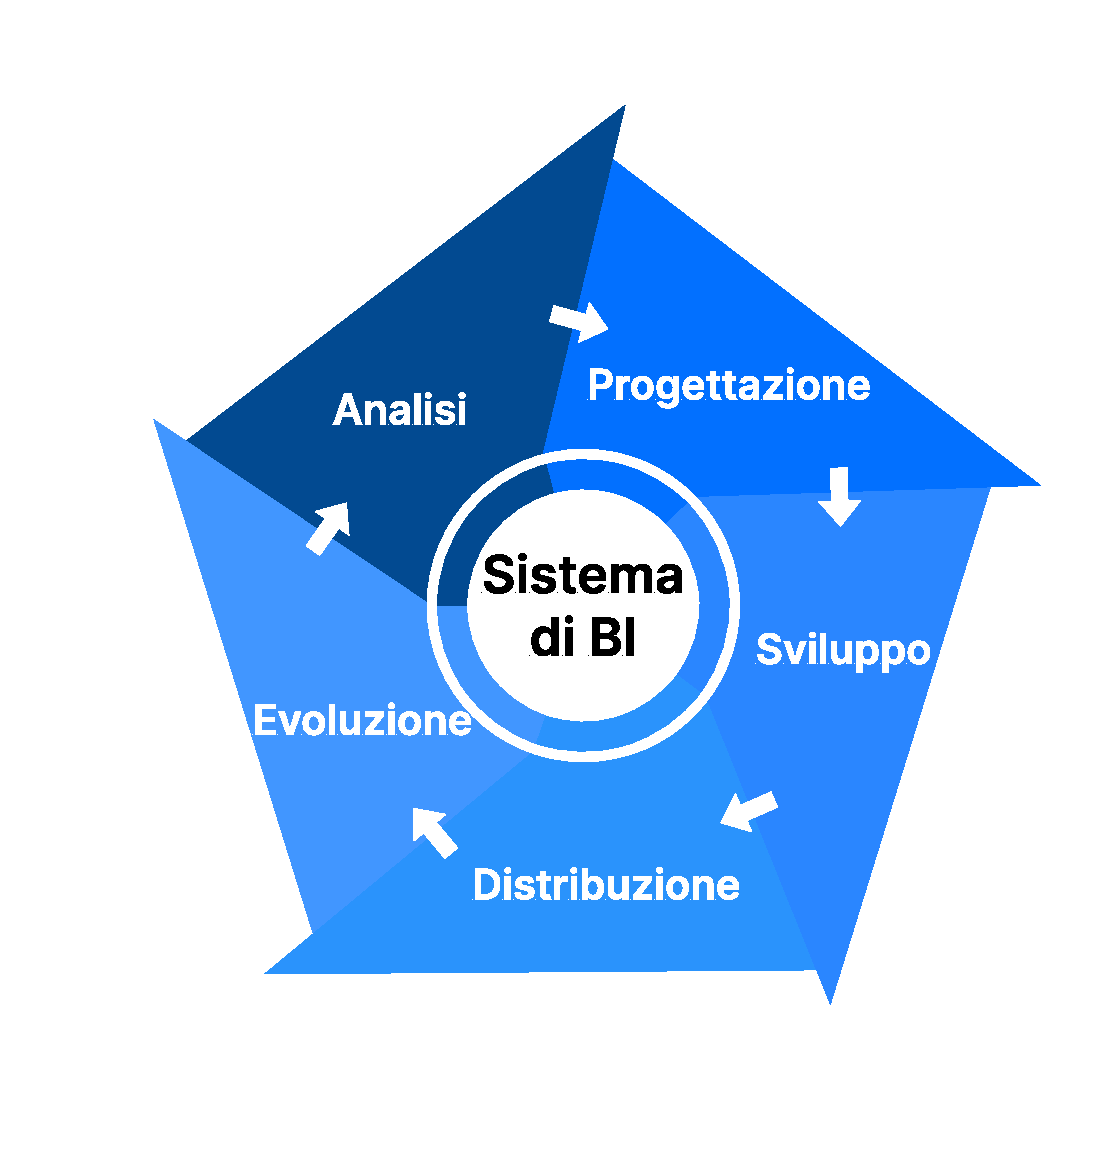
\includegraphics[width=0.75\linewidth]{figure//capitolo_3/Business Intelligence Life Cycle.pdf}
    \caption{Ciclo di vita di un processo di Business Intelligence}
    \label{fig:Business Intelligence Life Cycle}
\end{figure}

\subsubsection{Modello approfondito}

In modo più approfondito, l'implementazione di un sistema di Business Intelligence si compone di 8 fasi differenti \cite{altexsoft_bi_implementation}:

\begin{enumerate}
    \item \textit{Introduzione della BI ai dipendenti e agli stackholder}. Per poter sfruttare a pieno un sistema di BI è necessario far apprendere a tutti gli stakeholder\footnote{Uno \textit{stakeholder} è una parte (individuo, gruppo o organizzazione) che ha interesse in un'azienda e può influenzare o essere influenzata dalle sue attività (ad esempio, investitori, dipendenti, clienti o fornitori) \cite{investopedia_stakeholder}}. Le sue possibili funzionalità ed obiettivi. A seguito di una prima spiegazione, è poi necessario identificare il problema che si vuole risolvere o analizzare.
    \item \textit{Definizione di obiettivi, KPI e requisiti}. Una volta identificato il problema che si vuole affrontare, è necessario definire quali sono gli obiettivi che si vogliono raggiungere e quali possono essere (ipoteticamente parlando) dei KPI e metriche di valutazione rilevanti nell'ambito di interesse (possono essere sia vincoli finanziari che indici di prestazione). Ciò permetterà di comprendere anche quali sono i requisiti necessari allo sviluppo ed utilizzo della soluzione ricercata.
    \item \textit{Scelta degli strumenti o di una soluzione personalizzata}. A seguito della definizione dei requisiti è possibile comprendere quale soluzione possa essere la migliore da adoperare nel proprio sistema. Esistono molte soluzioni, tuttavia una soluzione personalizzata ad hoc per un'azienda può essere la scelta più adatta. Per comprendere quale sia la soluzione più conveniente è necessario svolgere una ricerca di mercato che permetta di mettere a paragone tutte le possibili scelte.
    \item \textit{Definizione di un team predisposto}. Per poter sfruttare al meglio un sistema del genere spesso è necessario definire un team predisposto a tale compito. Solitamente si cerca di inserire nel team personale di differenti reparti in modo da avere un possibile contatto diretto con gli stessi e personale conoscente del proprio ambito di lavoro. Inoltre, l'eterogeneità del gruppo permetterà una possibile evoluzione dello stesso grazie a punti di vista e pensieri differenti.
    \item \textit{Documentazione della strategia adottata}. Per creare un sistema nel modo corretto e senza errori, all'interno del progetto in questione viene adottata una specifica strategia. Tale strategia può includere differenti componenti, per questo motivo è importante riportare una documentazione che spieghi per ognuno di essi l'approccio adottato a riguardo. Ciò permette di semplificare la manutenibilità del sistema stesso.
    \item \textit{Configurazione di strumenti di integrazione e data warehouse e scelta di un approccio architetturale}. Tale fase dipende molto dallo strumento adottato, una scelta personalizzata o una plug and play avranno impatti differenti sulla difficoltà e capacità di integrazione con le infrastrutture e software dell'azienda.
    \item \textit{Implementazione di un'interfaccia utente finale}. In questa fase i dati vengono modellati, gestiti e infine messi a disposizione degli utenti finali grazie ad un'apposita interfaccia degli strumenti di BI. La creazione di corretti report è una fase essenziale e critica dell'intero processo perché permette l'analisi e la comprensione delle informazioni necessarie a prendere decisioni basate su tutti i dati gestiti dal sistema.
    \item \textit{Formazione degli utenti finali}. Un'ulteriore fase che può essere affrontata è la formazione degli utenti finali in modo da agevolare l'interazione e integrazione degli strumenti nei normali processi di gestione e sviluppo del personale aziendale. In caso contrario, si potrebbe riscontrare un problema di un utilizzo scorretto o sbagliato da parte degli utenti dello strumento messo a disposizione.
\end{enumerate}

\begin{figure} [H]
    \centering
    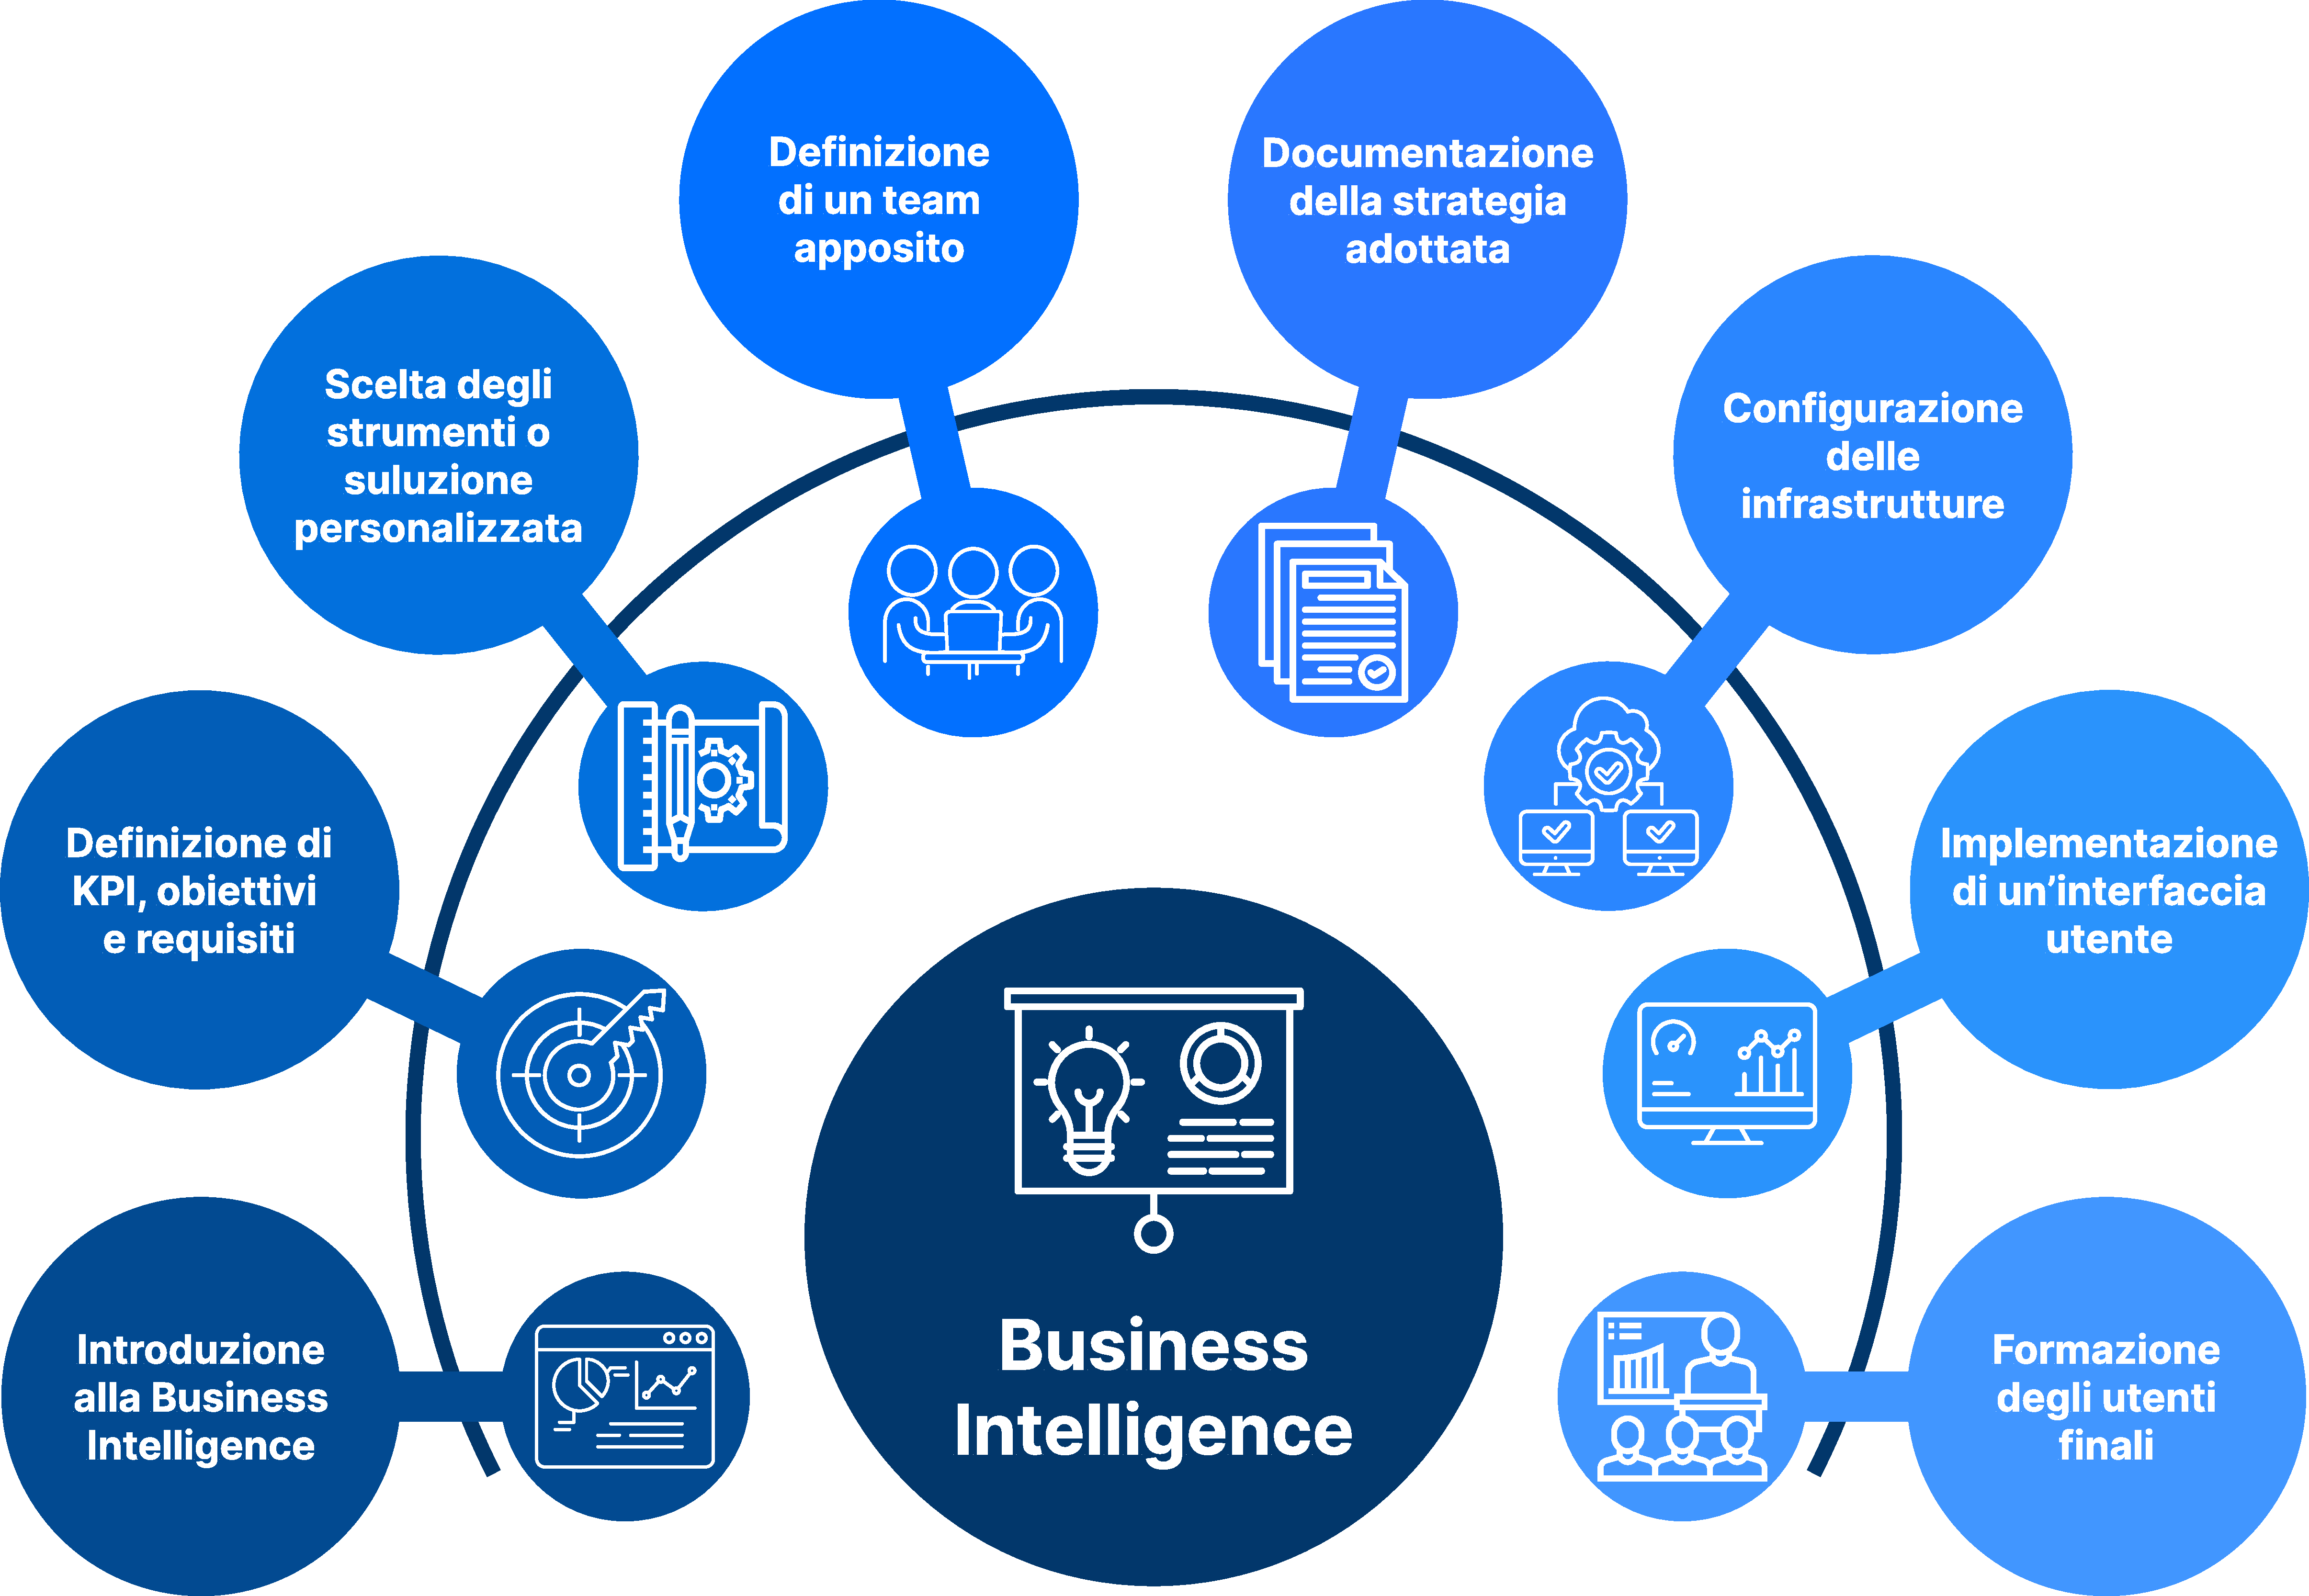
\includegraphics[width=1\linewidth]{figure//capitolo_3/Business Intelligence Process.pdf}
    \caption{Processo di adozione di un sistema di Business Intelligence}
    \label{fig:enter-labelBusiness Intelligence Process}
\end{figure}

\subsection{Le capacità della BI}

Le capacità della Business Intelligence sono competenze fondamentali che aiutano le aziende a migliorare la propria attitudine all'adattamento al cambiamento e all'esecuzione. Per quanto siano molte le ricerche a riguardo, è rimasto in gran parte silente il ruolo delle capacità della BI nel raggiungere l'adeguato abbinamento tra la BI e l'ambiente decisionale in cui è implementata.
Di seguito sono riportate le capacità prima accennate \cite{bi_capabilities}:

\begin{itemize}
    \item \textit{Qualità dei dati}. La BI si basa principalmente sui dati numerici, che vengono analizzati, gestiti e misurati. Proprio per questo motivo la qualità dei dati è un requisito fondamentale ed imprescindibile in questo mondo. Quando si parla di qualità dei dati si intende che essi siano consistenti e completi, perché diversamente non avrebbero una grossa affidabilità.
    \item \textit{Integrazione con altri sistemi}. Poiché il sistema di BI dipende da altri sistemi, un'importante caratteristica è la sua capacità di interoperabilità con questi. In questo caso, quando si parla di integrazione, si intende sia in ambito software che in ambito hardware.
    \item \textit{Accesso per gli utenti}. Dato che i sistemi di BI non hanno un solo utilizzo, obiettivo o scopo, non è possibile creare una soluzione onnicomprensiva adattabile a tutti i problemi. Per questo motivo è congeniale mettere a disposizione di utenti diversi gli strumenti di BI, in modo che questi possano creare i propri report e svolgere le relative analisi in totale autonomia senza alcuna difficoltà.
    \item \textit{Flessibilità}. Per far sì che una soluzione sia ottimale, è necessario che questa si adatti alle necessità e all'evoluzione dei dati e dell'organizzazione stessa (tecnologie e normative da dover applicare).
    \item \textit{Supporto alla gestione del rischio}. La gestione del rischio permette di aiutare nella presa di decisioni in condizioni spesso incerte. Questa capacità è cruciale per le organizzazioni che operano in ambienti ad alto rischio. Poiché nonostante esistano rischi e instabilità in ogni decisione aziendale, le compagnie cercano di adottare qualsiasi sistema che possa diminuire tale rischio, e la BI è uno di questi.
\end{itemize}

\subsection{BPI}

La progettazione dei processi e le tecnologie di automazione vengono sempre più utilizzate dalle aziende che cercano di migliorare le qualità e l'efficienza dei loro processi amministrativi e produttivi e fornire rapidamente e in modo affidabile servizi alle aziende e ai clienti individuali. Per svolgere queste attività al meglio, sono molte le aziende che decidono di adottare delle soluzioni che prendono il nome di \textbf{Business Process intelligence} (\textit{BPI}). Con questo termine si fa riferimento all'applicazione di tecniche di BI per lo sviluppo e l'implementazione di processi aziendali e comprende molte ambiti di applicazione (ad esempio, monitoraggio, analisi e scoperta dei processi, controllo di conformità, operazioni di previsione ed ottimizzazione), ovvero nell'ambito della \textit{BPM}\footnote{Il \textit{Business Process Management} (\textit{BPM}) è una disciplina che adotta diversi metodi per scoprire, modellare, analizzare, misurare, migliorare e ottimizzare i processi aziendali \cite{gartner_bpm}} \cite{academiaedu_bpi_definition}.

\begin{figure}[H]
    \centering
    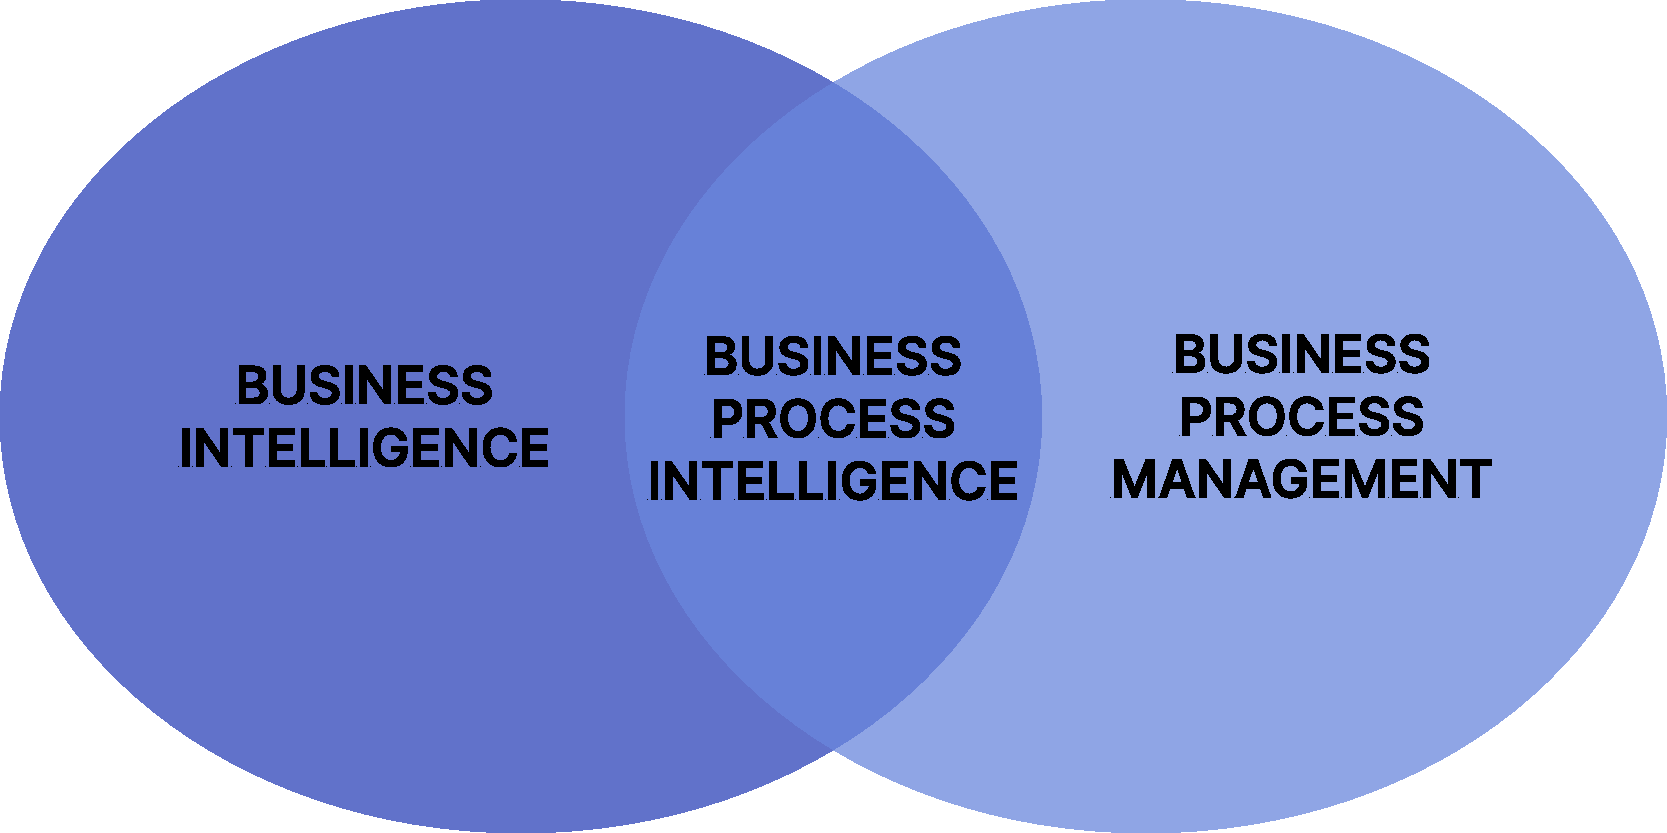
\includegraphics[width=0.75\linewidth]{figure//capitolo_3/Business Process Intelligence.pdf}
    \caption{La Business Process Intelligence}
    \label{fig:Business Process Intelligence}
\end{figure}

Date le molteplici possibilità e l'elevato spettro di applicazione, la business process intelligence dispone di diverse funzionalità che offrono altrettanti livelli di automazione per la gestione della qualità dei processi, ovvero \cite{academiaedu_bpi_feautures}:

\begin{itemize}
    \item \textit{Analisi}. La BPI permette agli utenti di analizzare le esecuzioni dei processi completati sia dal punto di vista aziendale che da quello programmatico per gli operatori IT. Inoltre, non solo offre molti sistemi di reportistica, ma la BPI permette anche di analizzare la progettazione di un modello di processo e identificare le tecniche per poterlo migliorare.
    \item \textit{Predizione}. La BPI permette di applicare modelli predittivi ai processi in esecuzione in modo da poter identificare preventivamente la possibilità di riscontrare eccezioni o comportamenti imprevisti e indesiderati. Anche in questo caso, è possibile avere un punto di vista aziendale oppure programmatico.
    \item \textit{Monitoraggio}. La BPI può monitorare ed analizzare le istanze dei processi che sono in esecuzione e informare l'utente nel caso vengano riscontrate situazioni insolite. Grazie a ciò, un utente può visualizzare e analizzare lo stato attuale del sistema, dei processi, dei servizi e delle risorse attualmente in uso e attività. Inoltre, con determinati principi di automazione, è possibile svolgere azioni predefinite in caso di situazioni critiche.
    \item \textit{Controllo}. La BPI, sfruttando il monitoraggio e la predizione dei processi, può interagire con il \textit{BPMS} (\textit{Business Process Management System}) per evitare delle degradazioni di qualità previste ed effettive.
    \item \textit{Ottimizzazione}. La BPI può individuare delle possibili aree di miglioramento nelle definizioni dei processi aziendali attualmente in uso e nell'assegnazione delle risorse ai relativi servizi in attività. Ciò permette una possibile diminuzione dei costi e un aumento dell'efficienza dei processi.
\end{itemize}

\subsection{La Business Analytics}

Oltre alla Business Intelligence, per quanto meno conosciuta, esiste anche la \textbf{Business Analytics} (\textbf{BA}) che comprende soluzioni adottate per definire modelli di analisi e simulazioni per creare scenari, comprendere realtà e prevedere possibili future situazioni. La BA include strumenti di data mining, analisi predittiva, analisi approfondita e statistica per essere fornita come un sistema di utilità per un'utente aziendale \cite{gartner_ba}.

A primo impatto la Business Analytics può sembrare identica alla Business Intelligence, ed effettivamente sono molto simili tra loro, tuttavia esiste una differenza minima quanto sostanziale, ovvero l'adozione dell'analisi predittiva con l'obiettivo di comprendere possibili eventi futuri. In altre parole, sia la BI che la BA sfruttano i dati di eventi e azioni passate ma lo fanno con scopi differenti: la prima focalizza il proprio obiettivo sul comprendere cosa sia accaduto in passato, mentre la seconda focalizza il proprio obiettivo sul comprendere come agire in futuro \cite{talend_bi_vs_ba}.


\subsubsection{Differenze tra BI e BA}
Per essere più precisi, è possibile affermare che la Business Intelligence adotta l'\textbf{analisi retrospettiva} (\textit{analisi diagnostica} e \textit{analisi descrittiva}), mentre la Business Analytics adotta l'\textbf{analisi prospettiva} (\textit{analisi prescrittiva} e \textit{analisi predittiva}) \cite{researchgate_bi_and_ba_analytics}.

Per comprendere meglio le differenze tra le due tipologie di analisi, di seguito è riportata una tabella riepilogativa:\cite{knowledgehut_bi_vs_ba}

\begin{comment}
\begin{table}
    \centering
    \begin{tabular}{ccc}
        Parametri & Business Intelligence & Business Analytics\\
        Definizione & 
        La BI riguarda la comprensione del passato e del presente di un'azienda.& La BA riguarda la previsione dei risultati futuri delle azioni intraprese dall'azienda.\\
        Focus & 
        Gli strumenti di BI si concentrano sulla gestione dei dati.& 
        Gli strumenti di BA si concentrano sull'analisi dei dati.\\
        Applicazioni & 
        Gli strumenti di BI sono progettati per fornire informazioni dettagliate sulle prestazioni della tua azienda nel tempo.&
        Gli strumenti di BA sono progettati per aiutare a prendere decisioni migliori su come ottimizzare le operazioni per il futuro.\\
        Approccio & 
        La BI si concentra sull'analisi diagnostica e sull'analisi descrittiva.& 
        La BA si concentra sull'analisi predittiva e sull'analisi prescrittiva.\\
        Utilizzo & 
        La BI si concentra in genere sul reporting a livello aziendale tra più dipartimenti e team.& 
        La BA in genere si concentra sull'analisi dettagliata di aree specifiche all'interno di un'organizzazione (ad esempio come il marketing).\\
    \end{tabular}
    \caption{Differenze tra Business Intelligence e Business Analytics}
    \label{tab:BI vs BA}
\end{table}
\end{comment}

%TODO: Controllare se va aggiunta qualche introduzione o prologo di collegamento

\section{La conoscenza}

Per migliaia di anni gli esseri umani hanno discusso sul significato di “\textit{conoscenza}”, su cosa significhi conoscere qualcosa e su come le persone possano generare e condividere nuova conoscenza. Nonostante l'importanza di tale dilemma nelle discussioni affrontate nel corso della storia, solo negli ultimi anni il mondo del business ha iniziato a riconoscere l'importanza della conoscenza come una risorsa \cite{knowledge_management_tools}.
La crescente evoluzione del mondo del Data Warehousing e dei Big Data ha portato alla necessità di svolgere studi, generare teorie o modelli e progettare strumenti che potessero aiutare le persone nell'estrazione di informazioni, ritenute, utili. Questa branca del mondo digitale prende il nome di \textbf{Knowledge Discovery in Databases} (\textit{KDD}), ovvero \textit{scoperta della conoscenza dei database}.

\subsection{La piramide della conoscenza}
Finora abbiamo parlato del mondo dell'analisi dei dati dando per scontato il concetto del legame tra i dati e la conoscenza, per quanto sia stata esplicitata più volta la loro rilevanza. «Tipicamente l'informazione è definita in termini di dati, la conoscenza in termini di informazione e la saggezza in termini di conoscenza», queste sono le parole della giornalista Jennifer Rowley \cite{rowley_dikw_hierarchy}, che permettono di descrivere brevemente la rappresentazione della \textit{piramide della conoscenza}, meglio conosciuta come \textbf{DIKW pyramid} (\textit{Data, Information, Kownledge and Windsome pyramid}), ovvero il modello creato per spiegare il processo di trasformazione dei dati e di come essi possano acquistare effettivamente, trasformandosi in informazione, conoscenza e saggezza.

\begin{figure}[H]
    \centering
    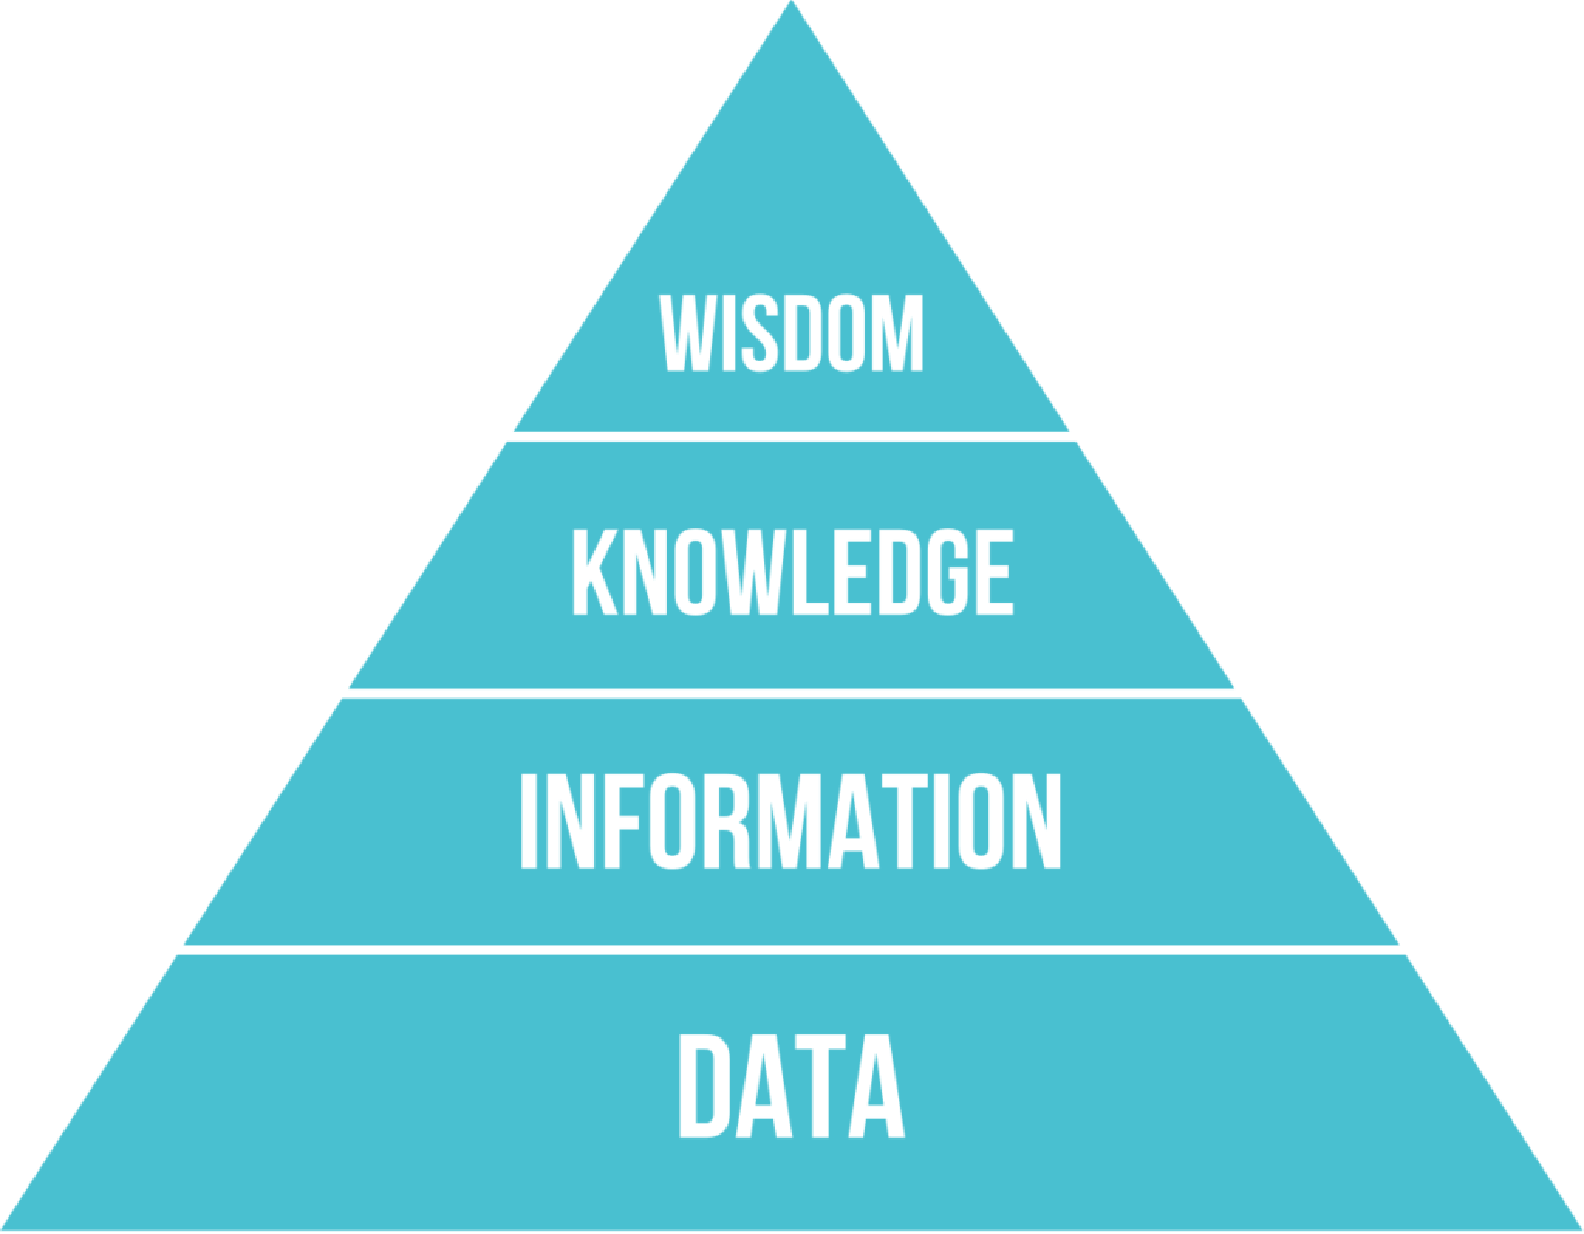
\includegraphics[width=0.6\linewidth]{figure//capitolo_3/DIKW Pyramid.pdf}
    \caption{Piramide della conoscenza}
    \label{fig:DIKW Pyramid}
\end{figure}

L'origine della piramide DIKW è incerta, è ignoto sia chi sia quando sia stata creata, come meglio spiegato dal professor Danny P. Wallace \cite{knowledge_management_historical} «La presentazione delle relazioni tra dati, informazioni, conoscenza e talvolta saggezza in una disposizione gerarchica fa parte del linguaggio della scienza dell'informazione da molti anni. Sebbene non sia chiaro quando e da chi tali relazioni siano state presentate per la prima volta come gerarchia, l'ubiquità della nozione di gerarchia è incorporato nell'uso dell'acronimo DIKW come rappresentazione abbreviata della trasformazione da dati a informazione a conoscenza in saggezza».

Per comprendere meglio tale rappresentazione, è meglio approfondire ognuno dei suoi elementi \cite{researchgate_revising_dikw_pyramid}:
\begin{enumerate}
    \item \textbf{Data} (\textit{Dati}). I dati sono solitamente definiti come fatti e statistiche che vengono ricavati insieme per svolgere riferimenti o analisi. I dati generalmente vengono combinati, ricombinati, confezionati, venduti, e ridistribuiti, proprio per questo motivo sono soggetti ad un uso improprio, quasi abuso. Inoltre, bisogna sempre ricordare che la raccolta di dati, anche in ordine di peta, exa o zettabyte, non ha alcun valore se essi possono essere inaccurati, obsoleti oppure intenzionalmente o non falsi. Proprio per questo motivo, i dati non portano sempre delle direttamente informazioni, ed è impossibile concludere che il volume di dati raccolto e archiviato per creare “informazioni” stiano effettivamente creando maggiori o migliori informazioni. È quindi possibile definire che i dati sono fondamentali perché il percorso verso le informazioni, la conoscenza e la saggezza si basa su di loro, tuttavia sono anche definibili inutili poiché da soli non hanno alcun valore.
    \item \textbf{Information} (\textit{Informazione}). Le informazioni, in termini generali, sono comunemente definite come fatti forniti o appresi su qualcosa o qualcuno. Nell'ambito digitale, l'informazione può essere definita come il significato attribuito dagli esseri umani ai dati raccolti o a sottoinsiemi selezionati di dati, tipicamente accompagnato da una presunzione di verità o di fatto. Pertanto, i dati interrogati possono diventare informazioni, ma se l'informazione sia utile o preziosa dipende interamente dal mondo di interrogazione dell'accuratezza dei dati sottostanti. Come espresso in precedenza, le informazioni possono definirsi valide solamente quando la fonte da cui provengono è valida, poiché altrimenti produrranno risultati errati. Ad aumentare l'importanza del valore delle informazioni vi è l'imprescindibile regola per cui per ottenere informazioni valide e utili dai dati è necessario svolgere le domande nel giusto modo e forma. La sbagliata interpretazione delle informazioni è uno scenario molto comune poiché è probabile che accada facilmente. Considerando quanto detto, l'informazione non porta necessariamente alla conoscenza e maggiori informazioni, per quanto corrette, non aumentano sempre la conoscenza. Pertanto, l'informazione potrebbe diventare conoscenza, ma non inevitabilmente o perlomeno non utile.
    \item \textbf{Knowledge} (\textit{Conoscenza}). La conoscenza è generalmente definita come fatti, informazioni e competenze apprese attraverso l'esperienza o l'istruzione. Data questa definizione, per quanto corretta, necessita di una precisazione, ovvero è possibile acquisire conoscenza su un argomento attraverso la raccolta di informazioni e le esperienze di vita, ma la conoscenza su un argomento non implica automaticamente la conoscenza su altri argomenti, anche se affini; per questo motivo il processo di acquisizione della conoscenza deve essere ripetuto su ogni argomento. In termini generali, maggiore è la conoscenza di una persona e più è probabile che soddisfi più bisogni umani e che ottenga ulteriore successo nella vita. Conoscenza e saggezza sono strettamente correlate, ma la saggezza comprende sia un volume più ampio che una maggiore durata di conoscenza accumulata.
    \item \textbf{Wisdom} (\textit{Saggezza}). La saggezza è comunemente definita come la qualità di avere esperienza, conoscenza e buon giudizio. A questa definizione si potrebbe aggiungere l'aggettivo “estesa”, poiché quantità limitate di questi elementi non sono sufficienti per creare saggezza. La saggezza si crea attraverso l'informazione, l'esperienza e la conoscenza, oltre all'apporto umano di analisi ed estrapolazione. L'uso intelligente dell'informazione, dell'esperienza e della conoscenza è vitale per la saggezza.
\end{enumerate}

\subsection{Gestione della conoscenza}

La \textbf{gestione della conoscenza} (\textit{GC}, o \textit{Knowledge Management – KM}) aziendale implica la gestione formale delle risorse di conoscenza per facilitarne l'accesso e il riutilizzo, generalmente adoperando tecnologie informatiche avanzate. Il KM viene definito formale in quanto la conoscenza viene classificata e categorizzata in base ad un'ontologia\footnote{L'\textit{ontologia} è lo studio dell'essere in quanto tale, nonché delle sue categorie fondamentali \cite{wikipedia_ontologia}.} prestabilita (che però è in continua evoluzione), in dati strutturati e semi-strutturati e in basi di conoscenza \cite{overview_of_knowledge_management}.

In altri termini, la gestione della conoscenza riguarda l'utilizzo della capacità intellettuale di un'organizzazione in modo sistematico e organizzato al fine di ottenere efficienze, garantire un vantaggio competitivo e stimolare l'innovazione \cite{ieee_enterprise_knowledge_management}.

Per essere più precisi è possibile fare riferimento alla definizione data da Gartner, ovvero: «La gestione della conoscenza è un processo aziendale che formalizza la gestione e l'utilizzo del patrimonio intellettuale di un'impresa. La KM promuove un approccio collaborativo e integrativo alla creazione, acquisizione, organizzazione, accesso e utilizzo delle risorse informative, inclusa la conoscenza tacita e non catturata delle persone» \cite{gartner_knowledge_management}.

\subsubsection{Fasi della gestione della conoscenza}

È possibile definire che tale procedimento si componga di quattro fasi principali, ovvero \cite{knowledge_management_process}:
\begin{enumerate}
    \item \textit{Acquisizione}. Tale fase corrisponde al processo organizzativo interno all'azienda che permette di facilitare la creazione della conoscenza tacita ed esplicita, partendo dalle persone della compagnia e integrando il livello organizzativo, associando il processo di identificazione di informazioni che creino una conoscenza proveniente dall'esterno.
    \item \textit{Archiviazione}. Tale fase corrisponde al processo di salvataggio delle conoscenze acquisite nella fase precedente all'interno di un apposito sistema che permetta di svolgere un'archiviazione di tale conoscenza in modo organizzato. Questa fase implica un processo di conversione che comporta organizzazione, strutturazione, archiviazione e combinazione della conoscenza al fine di facilitarne l'uso da parte degli utenti finali che dovranno necessitarne.
    \item \textit{Distribuzione}. Tale fase corrisponde al processo di condivisione delle informazioni salvate con l'obiettivo di portare alla creazione di nuove conoscenze derivanti dalle prime. Il solo possesso di conoscenza da parte di un'azienda non è di per sé sufficiente, quest'ultima dovrebbe garantire il flusso delle informazioni al fine di permettere un apprendimento tra gli individui, comportando un miglioramento delle prestazioni nel procedimento di gestione delle stesse. Il modo più efficace per diffondere la conoscenza è attraverso una metodologia che consenta un trasferimento sistematico.
    \item \textit{Utilizzo}. Tale fase corrisponde al processo di sfruttamento delle fasi precedenti per far sì che l'acquisizione della conoscenza possa essere utilizzata come base per lo sviluppo di nuove conoscenze attraverso l'integrazione, l'innovazione, la creazione e l'estensione della conoscenza pregressa. Per tale motivo, l'uso della conoscenza può definirsi tale quando attraverso esso vengono prese decisioni o apportate migliorie.
\end{enumerate}

\begin{figure}[H]
    \centering
    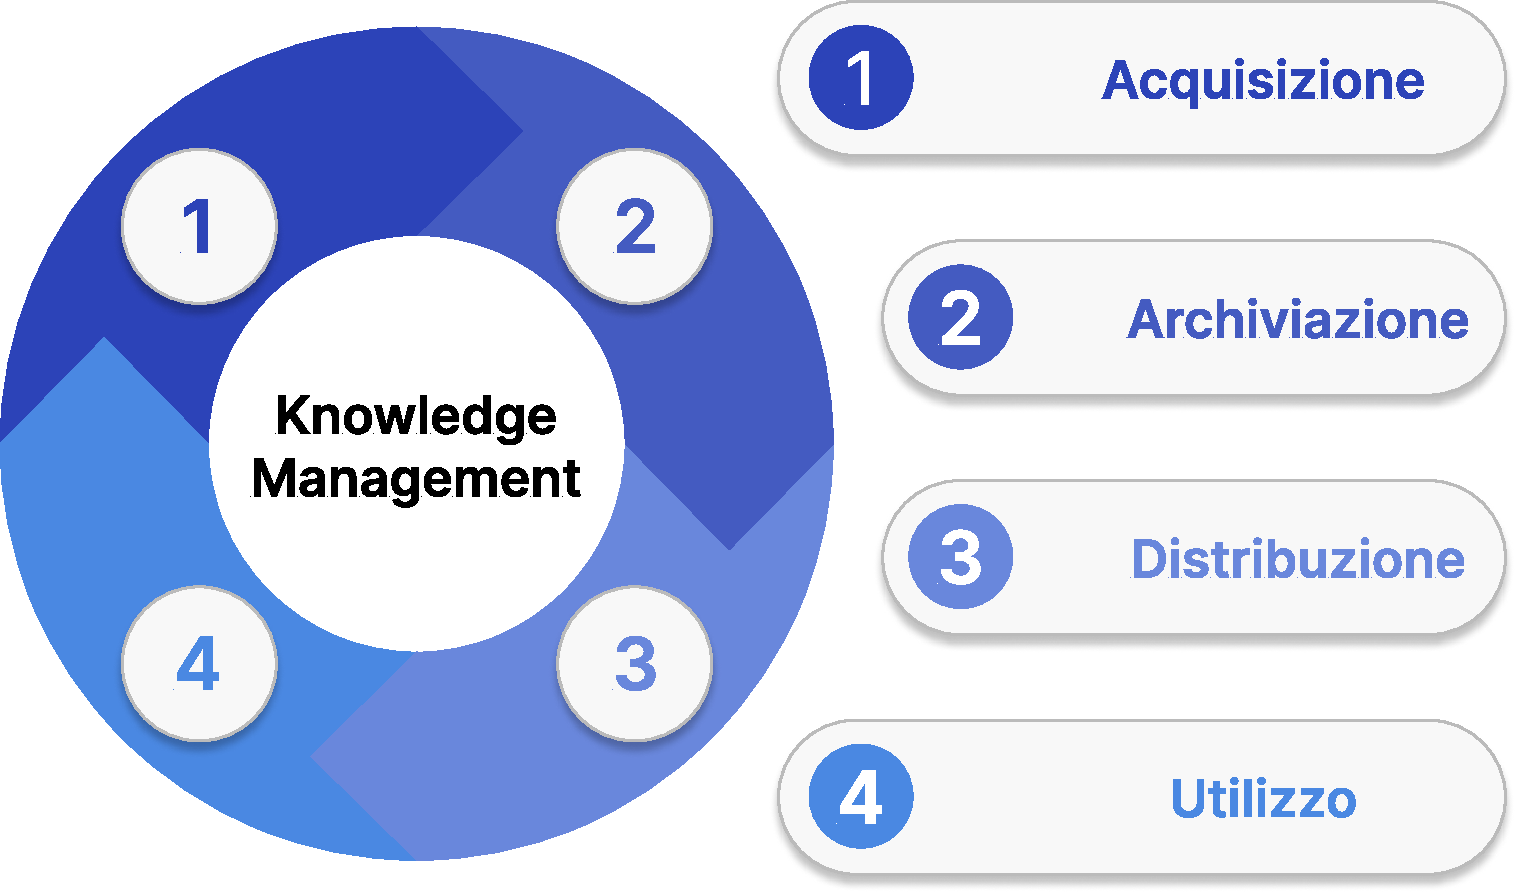
\includegraphics[width=0.8\linewidth]{figure//capitolo_3/Knowledge Management Process.pdf}
    \caption{Ciclo dell'informazione}
    \label{fig:Knowledge Management Process}
\end{figure}

\subsection{Sistemi per la gestione della conoscenza}

Prima dell'avvento della tecnologia, la gestione della conoscenza avveniva attraverso canali di comunicazione analogici e la conservazione di tale conoscenza era lasciata alle biblioteche. Tuttavia, con l'evoluzione della scienza è stato possibile per l'uomo di disporre di strumenti tecnologici che potessero semplificare tale compito, comportando cambiamenti non solo nel sistema di archiviazione ma anche nelle metodologie da applicare per svolgere tale compito. A questo scopo sono nati degli applicativi che permettessero di supportare le fasi del ciclo dell'informazione e della sua gestione.

Più precisamente, un \textbf{sistema di gestione della conoscenza} (\textit{Knowledge Management System, KMS}) sfrutta la conoscenza collettiva dell'azienda per portare migliori efficienze operative. Tali sistemi sono supportati dall'utilizzo di una conoscenza di base. Di solito sono fondamentali per una gestione efficiente ed efficace della conoscenza in questione, creando un ambiente centralizzato per memorizzare le informazioni e accedervi velocemente secondo le necessità del caso \cite{ibm_knowledge_management}.

\subsection{Scoperta della conoscenza nei database (Knowledge Discovery in Databases)}

A livello astratto, il campo del KDD si occupa dello sviluppo di metodi e tecniche per dare senso ai dati. Il problema di base affrontato dal processo KDD consiste nel mappare dati a basso livello (che sono tipicamente troppo voluminosi per essere compresi e assimilati facilmente) in altre forme che potrebbero essere più compatte, più astratte o più utili. Al centro del processo c'è l'applicazione di specifici metodi di data mining per la scoperta e l'estrazione di pattern \cite{from_data_mining_to_knowledge_discovery}.

La frase “\textit{knowledge discovery in databases}” viene attribuita al data scientist Usama Fayyad a seguito di un workshop tenuto nel 1989, dove venne usata per esplicitare che il risultato finale dell'indagine sui dati dovrebbe essere la scoperta di conoscenze utilizzabili. La KDD comprende tutti i processi, automatizzati e non, che migliorano o consentono l'esplorazione di database (indipendentemente dalle loro dimensioni), per recuperare potenziali conoscenze \cite{knowledge_discovery_in_databases}.

\subsubsection{Il processo KDD}

Il processo KDD è di tipo iterativo e interattivo (dove molte delle decisioni sono dipendenti dalle scelte dell'utente) e coinvolge nove differenti fasi, ovvero:\cite{researchgate_data_mining_and_knowledge}

\begin{enumerate}
    \item \textit{Apprendimento del dominio dell'applicazione}. Questa fase comprende lo sviluppo della comprensione delle conoscenze pregresse pertinenti e degli obiettivi dell'applicazione.
    \item \textit{Creazione di un set di dati target}. Questa fase include la selezione di un set di dati o la focalizzazione su un sottoinsieme di dati su cui bisogna effettuare la scoperta della conoscenza.
    \item \textit{Pulizia e pre-elaborazione dei dati}. Questa fase svolge le operazioni di base per la pulizia dei dati, la raccolta di informazioni utili alla modellazione, la definizione di regole per la gestione dei campi mancanti e la gestione del database.
    \item \textit{Riduzione e proiezione dei dati}. Questa fase comprende la ricerca di caratteristiche utili per rappresentare i dati e l'uso di metodi per la diminuzione delle dimensioni o del numero di variabili da prendere in considerazione.
    \item \textit{Scelta della funzione di data mining}. Questa fase si occupa di decidere lo scopo del modello derivato dall'applicazione dell'algoritmo di data mining.
    Scelta dell'algoritmo di data mining. Questa fase include la selezione dei metodi da adoperare per cercare modelli nei dati.
    \item \textit{Data mining}. Questa fase effettua la ricerca dei modelli di interesse in una particolare forma di rappresentazione o in un insieme di tali rappresentazioni.
    \item \textit{Interpretazione}. Questa fase comprende l'interpretazione dei modelli scoperti dalla fase precedente e, se necessario, la riapplicazione di alcune delle fasi già svolte.
    \item \textit{Utilizzo della conoscenza scoperta}. Questa fase include l'integrazione della conoscenza appresa nel sistema di performance, intraprendendo azioni basate s tale conoscenza o semplicemente documentarla.
\end{enumerate}

In generale è possibile raggruppare queste fasi in cinque passaggi essenziali che permettono di descrivere a pieno il processo KDD, ovvero \cite{knowledge_science}:

\begin{enumerate}
    \item \textit{Comprendere il dominio dell'applicazione per formulare il problema}. Questo è chiaramente il prerequisito per recuperare informazioni utili e scegliere dei metodi appropriati di apprendimento automatico ed estrazione dati, dipendentemente dallo scopo finale dell'applicazione e dalla natura dei dati di origine.
    \item \textit{Raccolta e pre-elaborazione dei dati}. Questo passaggio comprende la selezione delle fonti dati, la rimozione di eventuali rumori e anomalie, la gestione di eventuali dati mancanti, la trasformazione e la riduzione del volume di dati. Date queste numerose operazioni, questo è il passaggio che richiede maggior tempo nell'intero processo.
    \item \textit{Data mining}. Questo passaggio è necessario per l'estrazione dei modelli o pattern nascosti dei dati.
    \item \textit{Interpretazione (o post-elaborazione) dei dati}. Questo passaggio si occupa di interpretare la conoscenza scoperta mediante l'uso dei metodi di natura induttiva. Gli esperimenti mostrano che i pattern o i modelli scoperti dai dati non sono sempre di interesse o utilizzo diretto, e il processo di KDD è necessariamente iterativo con la valutazione della conoscenza scoperta.
    \item \textit{Applicazione delle conoscenze}. In alcuni casi, non è necessario adoperare sistemi informativi per sfruttare la conoscenza scoperta, mentre in altri casi l'utente può aspettarsi che questa possa essere inserita nei propri dispositivi di analisi per essere messa a disposizione di diversi programmi.
\end{enumerate}

\begin{figure}[!h]
    \centering
    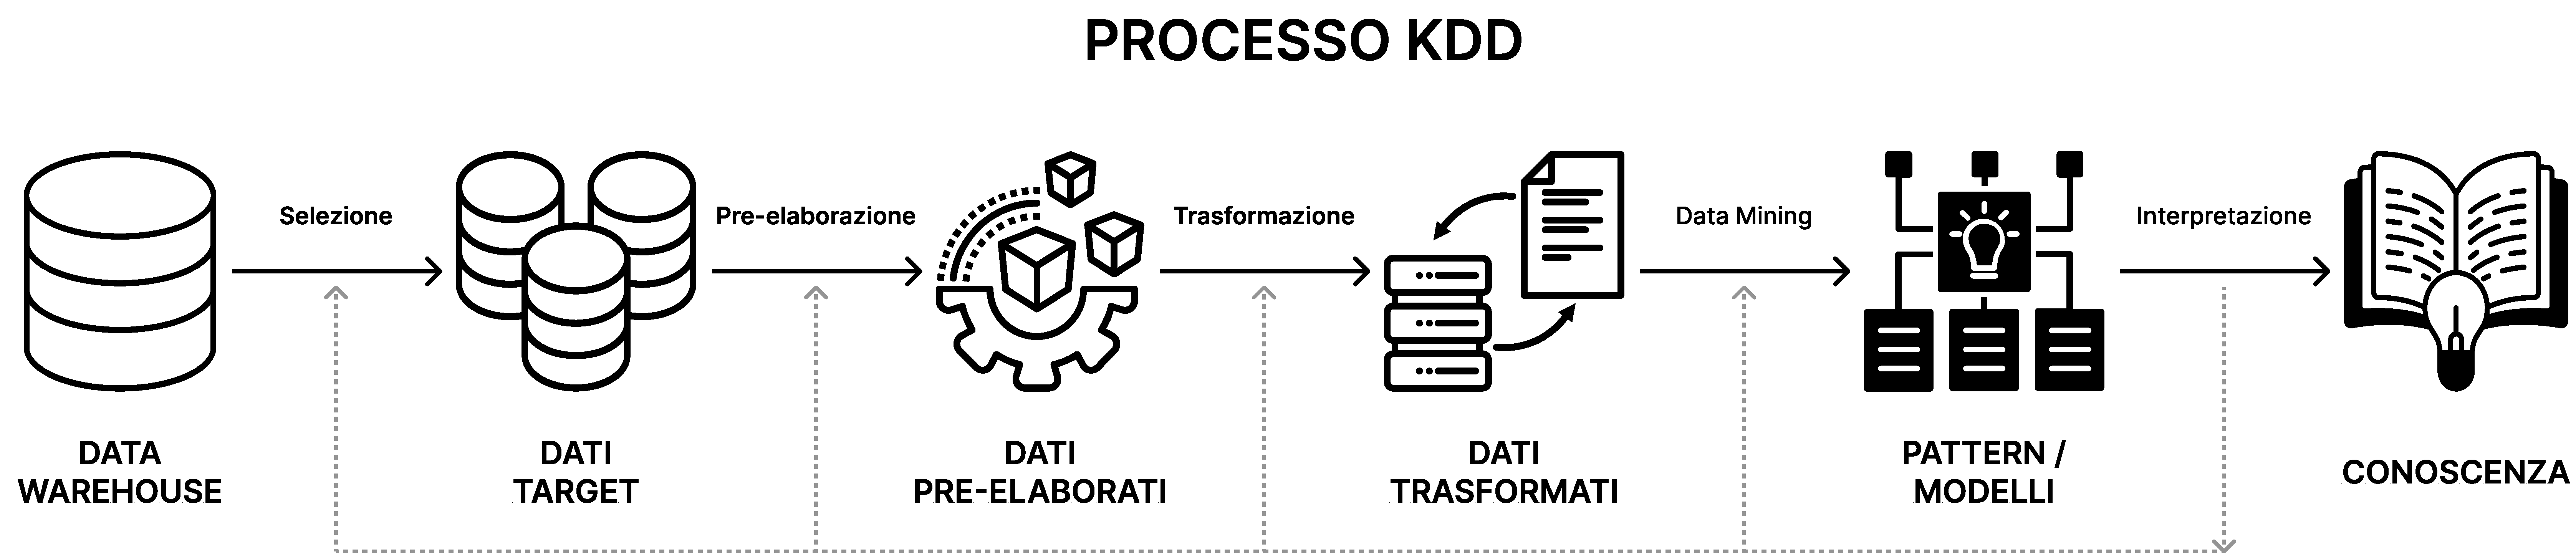
\includegraphics[width=1\linewidth]{figure//capitolo_3/KDD Process.pdf}
    \caption{Processo KDD}
    \label{fig:KDD Process}
\end{figure}

\subsection{Data Mining}

Il \textbf{Data Mining} (\textit{DM}) è la fase di estrazione della conoscenza, essenziale in un processo di KDD, da una grande quantità di dati oppure un data warehouse. Per effettuare questa estrazione, il data mining combina l'intelligenza artificiale, l'analisi statistica e i DBMS nel tentativo di estrarre conoscenze dai dati archiviati. Più semplicemente, è possibile dire che il DM è il processo di applicazione di specifici metodi per estrarre dei pattern dai dati \cite{citeseerx_data_mining}.

Secondo Fayyad, il Data Mining svolge sei principali funzioni \cite{aircconline_data_mining}:

\begin{enumerate}
    \item \textit{Classificazione}: consiste nel trovare modelli che analizzano e classificano uno specifico dato in diverse classi predefinite.
    \item \textit{Regressione}: consiste nell'associare uno specifico dato ad una variabile di previsione con valori reali.
    \item \textit{Clustering}: consiste nell'identificare un insieme finito di categorie o cluster per descrivere i dati.
    \item \textit{Modellazione delle dipendenze} (apprendimento delle regole di associazione): consiste nel trovare un modello che descriva dipendenze significative tra le variabili.
    \item \textit{Rilevamento delle deviazioni} (rilevamento delle anomalie): consiste nello scoprire i cambiamenti più significativi nei dati.
    \item \textit{Riepilogo}: consiste nel trovare una descrizione compatta per un sottoinsieme di dati.
\end{enumerate}

\subsubsection{Differenza tra Data Mining e KDD}

Dato questa introduzione è possibile comprendere come il termine “Data Mining” è improprio rispetto al processo in sé che ha l'obiettivo, non di estrarre i dati, bensì sfruttare gli archivi di dati, laddove ne sia presente una grande quantità, per estrarne il significato o ricavarne una conoscenza che possa essere definita preziosa \cite{aws_data_mining}.

Dato che molto spesso si fa confusione con i termini e le definizioni di KDD e DM, di seguito è riportata una tabella riassuntiva che permette di capirne le differenze \cite{geeksforgeeks_data_mining}:

\begin{comment}
\begin{table}[!h]
    \centering
    \begin{tabular}{ccc}
        Parametro & KDD & DM\\
        Definizione & Processo di identificazione di modelli e relazioni validi, nuovi, potenzialmente utili e comprensibili nei dati. & Processo di estrazione di informazioni o modelli utili e preziosi da set di dati di grandi dimensioni.\\
        Obiettivo & Trovare conoscenza utile dai dati. & Per estrarre informazioni utili dai dati.\\
        Tecniche adoperate & Pulizia, integrazione, selezione, trasformazione dei dati, data mining, valutazione dei modelli e rappresentazione e visualizzazione della conoscenza. & Regole di associazione, classificazione, clustering, regressione, alberi decisionali, reti neurali e riduzione delle dimensioni dei dati.\\
        Output & Informazioni strutturate, come regole e modelli, che possono essere utilizzate per prendere decisioni o previsioni. & Modelli, associazioni o intuizioni che possono essere utilizzati per migliorare il processo decisionale o la comprensione.\\
    \end{tabular}
    \caption{Differenze tra il processo KDD ed il Data Mining}
    \label{tab:kdd_vs_data_mining}
\end{table}
\end{comment}
\chapter{Sviluppo ``BI-CallReport'' per Azienda Acca Software}
\label{ch:Project}

A seguito del completamento dello studio svolto, precedentemente riportato, è stato svolto in incontro con i responsabili dei reparti interessati dell'azienda in modo da poter presentare e discutere riguardo gli argomenti trattati. Durante l'incontro sono stati illustrati i punti salienti dello studio, mettendo in chiaro i pro e i contro di ogni aspetto analizzato. Tale presentazione ha permesso ai decision maker aziendali di comprendere, in linee generali, quali sono tutte le funzionalità, i sistemi, e le possibilità che strumenti di \textit{Big Data}, \textit{Data Warehousing} e \textit{Data Analytics} possono portare all'interno di una compagnia. 

Una volta apprese le informazioni, è stato quindi svolto una riunione allo scopo di indicare l'obiettivo e le esigenze aziendali così da poter iniziare la seconda parte della commissione, ovvero l'implementazione di una soluzione che permettesse di risolvere tutte le problematiche e di migliorare lo stato attuale dell'azienda. Il briefing ha avuto lo scopo di coinvolgere i vari partecipanti nell'attuazione del progetto, assegnando ruoli e responsabilità, definendo tempi e modalità, stabilendo indicatori di performance e criteri di valutazione.

Questo capitolo espone la fase di progettazione e implementazione del progetto. Lo scopo è di fornire una panoramica generale del processo che ha portato alla definizione del progetto in questione, evidenziandone le motivazioni, le sfide e le opportunità che lo hanno caratterizzato ed ispirato.

\section{Definizione degli Obiettivi e dei Requisiti}

A seguito della presentazione svolta per mostrare tutte le possibilità del mondo dell'analisi dei dati è stato quindi compreso fin dal primo momento quale fosse il punto focalizzante dove l'azienda avrebbe dovuto puntare per migliorare nel proprio business, ovvero l'ambito del supporto tecnico fornito agli utenti. Quindi, per completare tale obiettivo è stato definito un progetto che avesse come fine il permettere al reparto di assistenza aziendale di migliorare dal punto di vista della gestione delle chiamate ricevute, così da poter soddisfare un maggior numero di utenza.

\subsection{Obiettivo del Progetto}

L'azienda fin dalla propria fondazione ha sempre messo al primo posto il rapporto con le persone, evitando che questo si limitasse alla mera interazione venditore-acquirente. La compagnia punta ad instaurare un rapporto di fiducia con i propri consumatori e per poter riuscire in tale compito la vendita di prodotti ad hoc pensati sulle loro esigenze non basta, è necessario permettere loro di risolvere ogni eventuale problema avendo a disposizione un professionista del settore che sia capace di instradarlo verso la risoluzione di ogni possibile riscontro. Seguendo questa politica, l'azienda ha sempre fornito una produzione di software sulle necessità degli utenti associato ad un apposito servizio clienti che fosse capace di soddisfare ogni evenienza.

Proprio per questa motivazione, è stato scelto come obiettivo la definizione di un BPI che avesse lo scopo di migliorare la gestione delle chiamate che i clienti svolgono per essere aiutati a seguito di essersi imbattuti in difficoltà che necessitassero dell'ausilio degli appositi addetti della compagnia. Per riuscire in tale compito è stato ipotizzato fosse necessario un sistema che permettesse di raccogliere in modo approfondito quale fosse il flusso delle chiamate ricevute e svolte tra l'azienda e i propri clienti. Grazie al recupero di tali dati sarebbe possibile applicare logiche di analisi sugli stessi in modo da comprendere eventuali difficoltà che il reparto di assistenza può incontrare come la congestione del servizio offerto a seguito di una larga richiesta per determinati argomenti o giorni, oppure comprendere quali fossero i software che necessitano di maggiore assistenza.

In altri termini, l'obiettivo del progetto era quella di creare un sistema che permettesse il salvataggio centralizzato e strutturato di dati in modo che questi potessero essere analizzati dipendentemente dalle necessità (dinamiche) sorte in passato o che potrebbero sorgere in futuro.

\subsection{Analisi dei Requisiti}

Nel definire lo scopo ultimo, il progetto ha delineato l'idea cardine su cui fondare il tutto, tuttavia essa non è abbastanza, per iniziare un progetto è necessario definire in modo preciso cosa si vuole realizzare, perché, come e con quali risorse a disposizione. Tale processo prende il nome di \textbf{analisi dei requisiti} e consiste nell'identificare e documentare le caratteristiche e funzionalità di cui lo stato finale del progetto deve essere caratterizzato.

L'analisi dei requisiti di un sistema è una metodologia strutturata per identificare un insieme appropriato di risorse che possa soddisfare le esigenze del sistema in questione e la definizione di requisiti per la progettazione o la selezione di tali risorse. I requisiti per un sistema o un elemento di un sistema sono catturati in una specifica. L’analisi dei requisiti è il processo attraverso il quale è possibile ricavare una visione approfondita del contenuto corretto della specifica così definita \cite{system_requirements_analysis}.
La fase della specifica dei requisiti, essendo le fondamenta sui il progetto si basa, è la più importante, dato che un errore può compromettere l'intero progetto. Per questo motivo la qualità di tale fase influisce in buona parte sulla qualità dell'intero prodotto finale. Perciò, scrivere una corretta \textit{specifica dei requisiti software} (o \textit{Software Requirements Specification, SRS}), ha un'importanza critica \cite{researchgate_srs_introduction}.

Non a caso, queste sono le parole di Frederick P. Brooks a riguardo \cite{brooks_srs}:

\begin{quote}
    «La parte più difficile del compito del software è arrivare a una specifica completa e coerente, e gran parte dell'essenza della creazione di un programma è infatti il debug della specifica.»
\end{quote}

Questa specifica deve essere sufficientemente chiara e non tecnica tale che possa essere compresa anche da persone non facenti parte del mondo dello sviluppo software e non ambigua, cosicché possa essere possibile analizzare le richieste strutturate con criterio ed evitare possibili fraintendimenti su quest'ultime in modo che il prodotto finale possa soddisfare le richieste iniziali \cite{researchgate_srs_structure}.

Per chiarire maggiormente cosa si intende con requisito, si riporta una delle molte definizioni esistenti, ovvero quella presente nel glossario di IEEE: «Una condizione o capacità che deve essere soddisfatta o posseduta da un sistema o da un componente del sistema per soddisfare un contratto, uno standard, una specifica o un altro documento formalmente imposto. L'insieme di tutti i requisiti costituisce la base per il successivo sviluppo del sistema o del componente del sistema.» \cite{software_requirements}. In altri termini, è possibile definire un requisito come una proprietà caratteristica di un sistema con lo scopo di risolvere una determinata problematica, riscontrata o eventualmente riscontrabile.

In generale, i requisiti di un sistema sono la combinazione di multipli requisiti provenienti da altrettante persone a diversi livelli di una compagnia o di ambito di interazione. Ciò, comporta che i requisiti variano nello scopo e nella proprietà che devono rispettare e per questo motivo si possono distinguere dipendentemente dal loro obiettivo in \cite{requirements_types}:

\begin{itemize}
    \item \textit{Requisito di prodotto}. Sono i requisiti derivanti da una necessità o un vincolo sul software da dover sviluppare (ad esempio, una funzionalità o simili).
    \item \textit{Requisito di processo}. Sono i requisiti derivanti da un vincolo sullo sviluppo stesso del software in questione (ad esempio, l'adozione di una determinata tecnologia).
\end{itemize}

Inoltre, possono essere distinti in base alla tipologia di vincolo che impongono rispondendo rispettivamente alla domande "cosa?" e "come?", ovvero:

\begin{itemize}
    \item \textit{\textbf{Requisiti funzionali}}. Tali requisiti, anche conosciuti con il termine di \textit{capacità}, descrivono le funzionalità che il software deve fornire. Può essere descritto come un requisito per il quale è possibile scrivere un insieme finito di passaggi di test per poterne convalidare il comportamento.
    \item \textit{\textbf{Requisiti non funzionali}}. Tali requisiti, anche conosciuti con il termine di \textit{vincoli}, servono per vincolare la soluzione a rispettare determinate caratteristiche/qualità. Possono essere classificati a loro volta dipendentemente se facciano riferimento alla sicurezza, all'affidabilità, all'interoperabilità, alle prestazioni, alla compatibilità, e molte altri.
\end{itemize}

\subsubsection{Requisiti Funzionali}

Di seguito sono riportati i requisiti funzionali definiti durante l'incontro:

\begin{itemize}
    \item \textbf{Acquisizione dei dati}. Il sistema deve essere in grado di acquisire dati da diverse fonti, compresi database, file di log e ulteriori sorgenti dove vengono originariamente salvati i dati.
    \item \textbf{Integrazione dei dati}. Il sistema deve permettere di integrare e consolidare dati provenienti da fonti differenti in un'unica struttura dati per garantire la coerenza e la completezza delle informazioni ricavate.
    \item \textbf{Archiviazione dei dati}. Il sistema deve fornire un meccanismo per l'archiviazione efficace e sicura dei dati, garantendo un accesso rapido ed efficiente.
    \item \textbf{Elaborazione dei dati}. Il sistema deve permettere l'esecuzione di operazioni di trasformazione, aggregazione e calcolo sui dati precedentemente archiviati per supportare analisi avanzate.
    \item \textbf{Storicizzazione dei dati}. Il sistema deve consentire la storicizzazione dei dati per analizzare l'evoluzione nel tempo delle metriche di assistenza tecnica, supportando in questo modo l'analisi di tendenza a lungo termine.
    \item \textbf{Ricerca dei dati}. Il sistema deve predisporre di funzionalità di ricerca per permettere agli utenti di trovare facilmente le informazioni di cui necessitano.
    \item \textbf{Interfaccia utente}. Il sistema deve fornire una interfaccia utente grafica (GUI) che consenta al personale preposto di accedere facilmente ai dati e alle analisi senza la necessità di competenze tecniche avanzate.
    \item \textbf{Generazione di report}. Il sistema deve permettere la creazione di report personalizzati in base alle esigenze specifiche del personale che accede al servizio.
    \item \textbf{Supporto di dashboard interattive}. Il sistema deve permettere la creazione di dashboard per monitorare in tempo reale le metriche chiave e facilitare la visualizzazione delle informazioni critiche.
\end{itemize}

\subsubsection{Requisiti Non Funzionali}
Di seguito sono riportati i requisiti non funzionali definiti durante l'incontro:

\begin{itemize}
    \item \textbf{Performance}. Il sistema deve garantire prestazioni elevate durante l'interrogazione e l'elaborazione dei dati, anche in caso di volumi considerevoli.
    \item \textbf{Scalabilità}. Il sistema deve essere progettato per gestire l'espansione dei dati nel tempo senza compromettere le prestazioni dello stesso.
    \item \textbf{Affidabilità}. Il sistema deve essere assicurare una disponibilità elevata del sistema e la capacità di ripristinare i dait in caso di guasti o interruzioni.
    \item \textbf{Usabilità}. Il sistema deve garantire un'interfaccia utente intuitiva e facile da usare in modo da ridurre al minimo il tempo di apprendimento per gli utenti finali.
    \item \textbf{Backup e ripristino}. Il sistema deve essere predisposto per l'adozione di procedure per il backup regolare dei dati e garantire la possibilità dell'eventuale ripristino in caso di perdita dei dati.
    \item \textbf{Manutenzione}. Il sistema deve fornire strumenti e procedure per la manutenzione regolare del sistema, inclusi aggiornamenti software e gestione delle versioni.
    \item \textbf{Training degli utenti}. Il sistema deve fornire sessioni di formazione per garantire che gli utenti siano adeguatamente preparati per utilizzare il sistema in modo efficace.
    \item \textbf{Tempi di risposta}. Il sistema deve permettere di svolgere interrogazioni e operazioni su dati in tempistiche definibili accettabili, garantendo in questo modo un'esperienza utente fluida e reattiva.
    \item \textbf{Documentazione adeguata}. Il sistema deve predisporre la presenza di una documentazione che sia sempre dettagliata e aggiornata sul sistema stesso (anche documentazione tecnica), cosi da semplificare la comprensione, manutenzione ed evoluzione del sistema nel tempo.
    \item \textbf{Manutenibilità}. Il sistema deve essere facile da mantenere, con la possibilità di aggiungere o modificare funzionalità senza che il servizio venga interrotto.
\end{itemize}

Questi requisiti hanno portato all'identificazione di un sistema composto da due elementi principali, ovvero: un Data Warehouse, che si occupa di svolgere il compito della gestione dei dati, e un software di Business Intelligence, che si occupa della visualizzazione, interrogazione e la generazione di dashboard e report dai dati in questione.

\section{Studio sulla Raccolta dei Dati}

La raccolta dei dati rappresenta la fase cardine su cui fondare la riuscita di un sistema di DW e BI. Per poter sapere come strutturare l'intero progetto è stato quindi necessario svolgere un procedimento di studio rispetto alle sorgenti di dati fruibili. L'attuale capitolo fornisce un'analisi approfondita delle metodologie e delle considerazioni coinvolte nello studio sulla raccolta dei dati per il progetto in questione.

\subsection{Obiettivi dello Studio}

Lo scopo principale dello studio sulla raccolta dei dati è naturalmente quello di definire in modo chiaro quali sono i dati rilevanti su cui svolgere il processo di ETL. In altre parole, definire il modo corretto per estrarre, trasformare e infine caricare i dati all'interno del data warehouse. Più precisamente, sono stati identificati i seguenti obiettivi su cui lo studio doveva focalizzarsi:

\begin{enumerate}
    \item \textit{Identificare le fonti dei dati}. Determinare le fonti dei dati, primarie e secondarie, pertinenti al reparto di assistenza tecnica.
    \item \textit{Definire la struttura dei dati}. Analizzare la struttura, il formato e lo schema dei dati nelle fonti identificate nel passaggio precedente.
    \item \textit{Valutare la qualità dei dati}. Analizzare la qualità delle fonti di dati e dei dati stessi, identificando e affrontando le eventuali problematiche scaturite dalla possibile incompletezza, inaccuratezza o incongruenza.
    \item \textit{Determinare la frequenza di aggiornamento}. Definire la frequenza con cui i dati devono essere estratti e caricati all'interno del DW per garantire che le informazioni siano sempre aggiornate.
\end{enumerate}

\subsection{Metodologia di Raccolta dei Dati}
Una volta definiti gli obiettivi è stato quindi il momento di definire le metodologie che potessero portarli a termine.
\begin{enumerate}
    \item \textit{Analisi delle fonti di dati}. In questo caso si precisano quali sono le metodologie necessarie per comprendere al meglio le fonti dei dati su cui operare. Più precisamente:
    \begin{itemize}
        \item File di log (fonte primarie e secondarie). Analizzare i file di log generati da Asterisk\footnote{Asterisk è un'implementazione software di un sistema PBX (Private Branch Exchange), ovvero un server che gestisce la rete telefonica privata di un'organizzazione.} per comprendere le operazioni svolte dagli utenti e dagli operatori, in modo da conoscere le informazioni generate dalla fonte principali dei dati.
        \item Database (fonti primarie e secondarie). Esaminare i database dove vengono salvate tutti i dati generati dal reparto di assistenza, così da identificare le tabelle pertinenti, principali e non, i campi chiavi e le relative relazioni.
        \item Sistemi di ticketing e reporting (fonti secondarie). Scandagliare i sistemi di ticketing e reporting per acquisire informazioni ulteriori sui problemi segnalati, lo stato delle risoluzioni e i tempi di intervento, in modo da avvalorare i dati fondamentali con ulteriori informazioni.
    \end{itemize}
    \item \textit{Progettazione dell'estrazione dei dati}. In questa fase è necessario vagliare quali sono le metodologie da attuare per l'estrazione dei dati focalizzandosi sui seguenti punti:
    \begin{itemize}
        \item Identificazione dei campi chiave. Definire i campi chiave per ogni fonte dati per facilitare l'integrazione e l'identificazione univoca dei dati che si vogliono recuperare.
        \item Filtraggio dei dati. Implementare dei filtri necessari per estrarre solamente i dati necessari, riducendo la quantità di dati inutili da recuperare e gestire nel sistema di data warehouse.
        \item Strategia di caricamento incrementale. Stabilire una strategia di caricamento incrementale per ridurre il carico, e quindi anche i tempi, di estrazione dei dati così da poter garantire un aggiornamento dei dati rapido ed efficiente.
    \end{itemize}
    \item \textit{Valutazione della qualità dei dati}. In questo punto è necessario comprendere al meglio i dati e la loro qualità in modo da sapere come doverli gestire e a quali potersi affidare maggiormente o meno. In modo più approfondito, le tipologie di analisi della qualità dei dati sono le seguenti:
    \begin{itemize}
        \item Analisi dei dati mancanti. Identificare e trattare i dati mancanti attraverso tecniche di imputazione o altre soluzioni appropriate.
        \item Controllo di qualità. Implementare controlli di qualità per rilevare errori nei dati durante il processo di estrazione, trasformazione e caricamento (ETL).
        \item Standardizzazione dei dati. Applicare regole di standardizzazione per garantire coerenza nei formati dei dati.
    \end{itemize}
\end{enumerate}

Come è stato riportato nella fase di studio, una comprensione approfondita delle fonti dei dati, la progettazione accurata dei processi di ETL e la valutazione precisa della qualità dei dati così gestiti sono punti fondamentali per garantire l'affidabilità e la pertinenza delle informazioni generate dagli stessi da parte del sistema. Per tale motivo, lo studio dei dati così proposto fornisce le basi per la messa in atto delle fasi successive di progettazione e relativa implementazione del sistema di data warehouse e delle soluzioni di business intelligence.

\section{Progettazione di un Sistema di Data Warehouse}

La creazione di un sistema di data warehousing è un processo complesso che coinvolge diverse fasi chiave, dalla pianificazione iniziale alla progettazione, implementazione e manutenzione continua. Per questo motivo è utile suddividere tale compito definendo le fasi che lo compongono. Nel nostro caso, tenendo conto la definizione degli obiettivi del progetto già precedentemente svolta, le fasi adottate sono state le seguenti:
\begin{enumerate}
    \item Scelta dell'architettura del sistema di data warehouse.
    \item Progettazione del modello dei dati.
    \item Selezione delle tecnologie.
    \item Implementazione e caricamento dei dati.
\end{enumerate}

\subsection{Scelta dell'Architettura del Sistema}

Grazie alle conoscenze acquisite con il precedente studio, è stato scelto di adottare un'architettura a due livelli in modo da avere una struttura solida, scalabile e performante ma allo stesso tempo non enormemente complessa se rapportata all'obiettivo del progetto.

Per avere una maggiore comprensione del tutto, si intende precisare che un sistema di data warehouse può essere suddiviso in modo generale in tre parti o livelli distinti, ovvero:

\begin{enumerate}
    \item \textit{Livello sorgente}. In tale livello sono situati tutte le fonti, eterogenee e non, da cui dover recuperare i dati da caricare all'interno del data warehouse.
    \item \textit{Livello del data warehouse}. In tale livello è presente il data warehouse vero e proprio dell'intero sistema, ovvero l'infrastruttura che si occupa di gestire i dati che si vogliono processare dalle fonti.
    \item \textit{Livello di analisi}. In tale livello sono presenti gli strumenti finali che si occupano di recuperare e gestire i dati ad alto livello per metterli a disposizione degli utenti finali.
\end{enumerate}

Un'architettura a uno, due o tre livelli identifica il numero di sottolivelli che caratterizzano il secondo livello, ovvero quello del DW. Nel nostro caso, adottando un'architettura a due livelli, esso viene suddiviso in un \textit{livello di alimentazione} e un \textit{livello di data warehouse}. Il primo sottolivello si occuperà di svolgere le operazioni di processamento dei dati, mentre il secondo si occuperà di salvare tutti i dati supportato da un contenitore di metadati. Nel nostro sistema è stato scelto di non adottare dei data mart poiché il progetto è momentaneamente ristretto ad un solo ambito di utilizzo e applicazione e quindi la scelta di aggiungerli avrebbe aumentato la complessità del progetto senza apportare alcun miglioramento o beneficio. Invece, il contenitore di metadati avrà un ruolo cruciale, come nella maggior parte dei sistemi, poiché avrà il compito di mantenere le informazioni sulle sorgenti, sui meccanismi di accesso, sulle procedure di pulitura, trasformazione e alimentazione, eventualmente sugli utenti, ecc.

\subsection{Progettazione del Modello dei Dati}

Tale fase è cruciale per la riuscita di un sistema di data warehousing poiché coinvolge la definizione di come i dati saranno strutturati all'interno del sistema e quindi come essi dovranno essere sfruttati per sopperire alle esigenze di analisi e reporting dei dati da parte degli utenti finali.

Come primo dubbio bisogna risolvere la scelta tra uno schema dimensionale oppure uno schema normalizzato. A tal proposito di seguito sono riportati i vantaggi e gli svantaggi riscontrati nell'analizzare entrambe le possibili scelte:

\begin{itemize}
    \item \textit{Schema Dimensionale}:
        \begin{itemize}
            \item Vantaggi:
                \begin{itemize}
                    \item Facilita le query analitiche complesse.
                    \item Semplifica la comprensione e navigazione per gli utenti finali.
                \end{itemize}
            \item Svantaggi:
                \begin{itemize}
                    \item Richiede maggiore spazio di archiviazione.
                \end{itemize}
        \end{itemize}
    \item \textit{Schema Normalizzato}:
            \begin{itemize}
            \item Vantaggi:
                \begin{itemize}
                    \item Minimizzazione della ridondanza dei dati.
                    \item Risparmio di spazio di archiviazione.
                    \item Manutenzione semplificata dei dati.
                \end{itemize}
            \item Svantaggi:
                \begin{itemize}
                    \item Maggiore complessità delle query analitiche.
                \end{itemize}
        \end{itemize}
\end{itemize}

Date queste analisi è stata scelta la seconda ipotesi, ovvero lo schema normalizzato, poiché il più affine rispetto alle seguenti scelte già preventivate:

\begin{enumerate}
    \item L'utente finale dovrà avere accesso unicamente al DSS messo a disposizione per svolgere analisi e report. Tale scelta comporta che qualsiasi complessità il sistema di data warehouse interno possa avere, esso dovrà essere completamente astratto rispetto al livello di presentazione adoperato degli utenti finali.
    \item È molto probabile che il sistema venga arricchito con ulteriori dati provenienti da fonti tuttora non considerate e per questo motivo necessiterà di manutenzione ed aggiornamento. Tale scelta comporta che l'eventuale utilizzo dello schema dimensionale possa comportare una maggiore difficoltà nella manutenzione ed aggiornamento.
    \item Per permettere una migliore interoperabilità con ulteriori futuri data mart da integrare nel data warehouse, oppure ulteriori utilizzi differenti da quello attualmente ipotizzato, mantenere i dati il meno ridondanti possibili e maggiormente uniformati è un importante compito ed obiettivo.
\end{enumerate}

\subsection{Selezione delle Tecnologie}

Come seconda fase è necessario scegliere quali tecnologie vogliono essere adottate per implementare il sistema. Sono diverse le tecnologie coinvolte nelle fasi di estrazione, trasformazione e caricamento (ETL), nella gestione del database di data warehouse e nelle attività di business intelligence. Più precisamente:

\begin{enumerate}
    \item \textit{Strumenti di ETL}. Come strumento di ETL è stato adottato uno strumento ad hoc custom. È stato preferito a degli strumenti messi a disposizione dal mercato attuale, i più comuni sono: \textit{Talend}, \textit{Apache NiFi} e \textit{Microsoft SSIS}, per motivi di massima personalizzazione in base alle esigenze.
    \item \textit{DBMS per il Data Warehouse}. Come DBMS per la gestione dei dati del sistema è stato adottato PostgreSQL, un database SQL relazionale. È stato preferito a database come \textit{Amazon Redshift}, \textit{Snowflake} o \textit{Google BigQuery} poiché per il momento l'azienda ha deciso, per questioni di privacy e sicurezza, di adottare soluzioni che permettessero di mantenere i dati all'interno della stessa. Tuttavia, se in futuro si decidesse di voler espandere le dimensioni e la complessità del progetto, sarà facilmente possibile adottare una soluzione come Amazon Redshift essendo quest'ultimo basato proprio su PostgreSQL.
    \item \textit{Strumenti di Business Intelligence}. Come strumento DSS per la BI è stato adottato Power BI, tra gli strumenti attualmente in commercio (altri sono \textit{Tableau}, \textit{Looker} o \textit{Datapine}). Tale scelta è dovuta dal fatto che è uno degli strumenti utilizzati da maggior tempo e con maggiore diffusione. Ciò permette di avere un software con aggiornamenti garantiti e sempre nuove funzionalità, aggiornabili anche aggiungendo add-on custom, che aumenteranno le possibilità del progetto stesso.
\end{enumerate}

Tali scelte sono dovute avendo preso in considerazione le seguenti motivazioni:
\begin{itemize}
    \item \textit{Compatibilità con l'infrastruttura esistente}. Le tecnologie selezionate si integrano senza problemi con l'infrastruttura IT esistente per garantire una transizione fluida.
    \item \textit{Scalabilità}. Le tecnologie sono in grado di scalare per gestire crescenti volumi di dati e carichi di, in termini accettabili tali da sopperire alla possibile richiesta del progetto.
    \item \textit{Facilità di utilizzo}. Gli strumenti e le piattaforme sono intuitivi e facilmente utilizzabili dagli utenti finali, riducendo la necessità di formazione estensiva.
    \item \textit{Prezzo e licenza}. Il costo totale di proprietà (TCO) delle tecnologie, compresi i costi di licenza, di implementazione e di manutenzione continua sono nulli o minimi rispetto ad una possibile evoluzione del servizio.
    \item \textit{Supporto della community e aggiornamenti}. Le tecnologie godono di un supporto attivo dalla community o dal fornitore e ricevono aggiornamenti regolari per rimanere al passo con le nuove tecnologie e correggere eventuali vulnerabilità.
    \item \textit{Facilità di Manutenzione}. Le tecnologie sono di facile gestione e manutenzione agevole per garantire un funzionamento continuo del sistema.
\end{itemize}

\section{Processo di ETL}

\subsection{Analisi del Processo di ETL}

Una volta preso atto delle risorse aziendali è quindi necessario delineare il processo di ETL per la gestione dei dati. Per quanto spesso sia dato per scontato questo compito non va sottovalutato, anche esso è un punto cruciale per la riuscita di un sistema di data warehousing. Come accennato in precedenza, questa fase si occupa di estrarre i dati dalle fonti originali, trasformarli in un formato adatto per l'analisi, e caricarli nel data warehouse. Di seguito si approfondiscono tutti i passaggi del processo di ETL:

\begin{enumerate}
    \item \textit{Estrazione}. La fase di estrazione, che si occupa del recupero dei dati dalle varie fonti messe a disposizione, è caratterizzata da:
    \begin{itemize}
        \item Tecniche. Sono di due tipi: \textit{estrazione completa}, che recupera ogni volta l'interezza dei dati della fonte, ed \textit{estrazione incrementale}, che recupera solo i dati nuovi, modificati o che in precedenza sono stati evitati.
        \item Metodologie. Esistono differenti tipologie di estrazione, le più comuni sono: esecuzione di \textit{query sui database}, scraping\footnote{Per scraping dei dati (o scraping) si intende una tecnica in cui un programma informatico estrae dei dati dall'output generato da un altro programma.\cite{cloudflare_scraping}} dai \textit{file di log} e svolgere \textit{richieste API} alle fonti che le espongono.
    \end{itemize}
    \item \textit{Trasformazione}. La fase di trasformazione, che si occupa del convertire i dati estratti in formati coerenti e facili da gestire, è caratterizzata da:
    \begin{itemize}
        \item \textit{Attività}. Le principali attività di trasformazione riguardano la \textit{pulizia}, la \textit{standardizzazione}, l'\textit{arricchimento} e l'\textit{aggregazione} dei dati recuperati in precedenza.
        \item \textit{Linguaggio}. Il linguaggio adottato nello svolere le attività elencate permette di essere più efficiente o semplice, dipendentemente dalla caratteristica che si ricerca.
        \item \textit{Strumenti}. Per riuscire in tale compito, è possibile adottare strumenti che permettono renderlo più semplice, intuitivo o immediato.
    \end{itemize}
    \item \textit{Caricamento}. La fase di caricamento o salvataggio, che si occupa di inserire i dati trasformati all'interno del data warehouse, è caratterizzata da:
    \begin{itemize}
        \item Metodologie. Quando si parla di metodologia di caricamento si fa riferimento alla possibilità di scegliere se caricare i dati in un formato \textit{batch}, ovvero caricati periodicamente a lotti, oppure in \textit{tempo reale}, inserendo ogni volta il singolo record recuperato e gestito.
        \item Approcci. In questo caso, per approccio al caricamento si intende il modo in cui si intende svolgerlo, ovvero se svolgere un \textit{caricamento completo} inserendo i dati solo quando tutti i dati sono stati estratti e trasformati, oppure se svolgere un \textit{caricamento incrementale} inserendo i dati  quando vengono gestiti volta per volta.
    \end{itemize}
\end{enumerate}

\subsection{Definizione delle Caratteristiche del Processo di ETL}

Date le caratteristiche sopracitate e le risorse messe a disposizione dall'azienda è stato necessario creare un sistema personalizzato che svolgesse il processo di ETL. Tale motivazione ha portato ad adottare un linguaggio di programmazione come Golang per scrivere il codice che si occupasse di tale compito. La scelta è ricaduta sul linguaggio ideato da Google poiché è efficiente, stabile e allo stesso tempo non complesso da adottare. Quindi in un'ottica di scalabilità del progetto, oppure di ampliamento del team ad ulteriori persone, con la giusta documentazione, tale compito non comporterebbe un effort elevato. Inoltre, tale programma, una volta completo, è stato caricato all'interno di un'immagine docker per poi essere hostato da un server aziendale in un container apposito, tale che le funzionalità predisposte siano sempre a disposizione degli utenti finali.

Il programma così creato si occupa di svolgere l'intero processo di ETL in modo iterativo ogni minuto, in modo da avere sempre dati aggiornati all'interno del data warehouse. Tale scelta, ha però comportato la necessità di dover gestire la possibilità di incontrare stati dei record incompleti o incongruenti, dato che l'aggiornamento delle risorse originali non viene svolto in modo sincronizzato. Per poter gestire tale problematica, il sistema oltre a caricare i dati in modo incrementale, in modo da non dover sempre gestire un alto carico di dati e da non sforzare le risorse nell'estrarre i dati, si occupa di caricare ogni volta le informazioni basilari recuperabili dalle fonti, per poi aggiornarle in un'iterazione successiva al recupero dei dati ulteriori da dover inserire per completare l'intero record finale. In questo modo, viene perso ogni possibilità di incongruenza o perdita dei dati che necessitasse che tutte le risorse avessero i dati al loro interno in contemporanea. Quindi, il sistema si occupa, ad ogni iterazione, di recuperare le informazioni da multiple fonti differenti (sia file di log che database) per poi svolgere operazioni di pulizia e formattazione, in modo da svolgere operazioni di caricamento incrementale e batch. La possibilità di far coincidere la metodologia e l'approccio di caricamento sopracitati è dovuta proprio al fatto che le iterazioni vengono svolte a poca distanza l'una dall'altra e per questo motivo i dati da gestire sono pochi ed un caricamento batchato comporta la necessità di dover svolgere un numero minore di operazioni senza che queste siano troppo pesanti.

\subsection{Motivazioni delle Decisioni Implementative}

Nel decidere quali approcci o caratteristiche adottare nel nostro sistema, sono state prese in considerazione le seguenti motivazioni:
\begin{itemize}
    \item \textit{Controllo di qualità dei dati}. Il sistema implementa controllo di qualità per garantire l'integrità e l'accuratezza dei dati rimuovendo ogni possibile refuso, dati che presentano formati contrastanti o errati, oppure dati che si compongono principalmente di informazioni che non risulterebbero necessarie o addirittura fuorvianti.
    \item \textit{Gestione degli errori}. Il sistema prevede meccanismi per gestire e registrare gli errori durante l'intero processo, insieme ad un sistema di logging, in modo da poter individuare immediatamente il problema e risolvere il tutto.
    \item \textit{Pianificazione e scheduling}. Con una corretta pianificazione e scheduling delle iterazioni che il sistema deve svolgere, è possibile definire le migliori finestre temporali predeterminate in modo da evitare impatti sulle comuni operazioni aziendali oppure aumentare o diminuire il tempo di differimento tra una esecuzione e un'altra in base alle necessità.
    \item \textit{Monitoraggio delle prestazioni}. Il programma permette di avere, anche grazie al sistema di logging interno sopracitato, la possibilità di monitorare le prestazioni dello stesso, in modo da poter comprendere se siano presenti dei rallentamenti in determinate attività svolte durante il processo di ETL, oppure se siano congestionate le risorse in quel momento.
    \item \textit{Gestione delle modifiche}. Il sistema mette a disposizione, degli operatori del settore, di modificare nel tempo le scelte delle attività da dover svolgere, in modo da permettere una personalizzazione approfondita e perfetta per le necessità mostrate degli utenti finali.
\end{itemize}

\section{Creazione di Dashboard e Report Finali}

\subsubsection{Scelta del DSS}

Una volta predisposto il data warehouse e creato il sistema che si occuperà del processo di ETL, è ora necessario adottare un sistema di DSS in modo da poter mettere a disposizione i dati agli utenti finali. Per riuscire in tale compito, è stato deciso di adottare il software di casa \textit{Microsoft} "\textbf{Power BI}". 

Come accennato in precedenza, tale scelta è dovuta alla grande importanza del software in questione nel mondo della Business Intelligence comportando una ampia diffusione dello stesso. Tuttavia, il suo largo utilizzo e sempre attiva community non sono le uniche motivazioni che hanno valorizzato la scelta. Il software in questione dispone sia di un'interfaccia Web sia di un'interfaccia desktop, da utilizzare offline, leggere e user-friendly. Questa doppia valenza, ci permette di strutturare il progetto dal punto di vista del livello più esterno in due fasi distinte, ovvero: 

\begin{enumerate}
    \item Una prima fase che limiterà l'utilizzo del software solamente agli utenti preposti ai quali sarà messa a disposizione l'applicazione e il file con all'interno le dashboard e i report creati. Ciò permetterà di mantenere un accesso controllato e limitato ai soli utenti principali adottando account personali per la visualizzazione delle informazioni.
    \item Una seconda fase che permetterà l'accesso all'interfaccia di reportistica tramite l'ausilio della piattaforma web hostando il tutto in un server interno grazie all'adozione del servizio "\textit{Server di report di Power BI}". Ciò permetterà di espandere l'accesso ad ulteriori utenti e tenerlo allo stesso tempo controllato, in modo da mantenere un servizio stabile e scalabile.
\end{enumerate}

\subsection{Caratteristiche delle Dashboard e Report da Creare}

La fase finale del progetto comprende l'unica parte di cui un utente finale ha visione e maggiore interesse. Proprio per tale motivo, riuscire a definire delle dashboard o report è un aspetto molto importante, poiché da questo dipenderà la facilità di comprensione e interattività con i decision maker. Per poter completare al meglio tale compito, è stata varata l'analisi dei seguenti punti:

\begin{enumerate}
    \item \textit{Definizione degli obiettivi}. Naturalmente, arrivati a questo punto è stato necessario approfondire con gli utenti finali quali fossero i KPI e i dati di loro interesse. Per tale motivo è quindi stato necessario definire le domande chiave che gli utenti avevano necessità di risolvere e gli obiettivi di business dell'organizzazione, così da poter delineare rispettivamente le dashboard e i report in base ai relativi bisogni.
    \item \textit{Progettazione dell'interfaccia utente}. Questa fase, grazie all'utilizzo di Power BI come software DSS permette di essere parzialmente completa in partenza e necessitando di una progettazione dell'interfaccia solo per quanto riguarda le dashboard e i report utilizzabili. Per questo motivo, in ogni dashboard è stato definito un design comune che permettesse agli utenti di familiarizzare con lo stesso e non dover approcciare ad un layout differente ad ogni interrogazione differente.
    \item \textit{Selezione delle visualizzazioni}. Mettendo alla base di questo punto la definizione degli obiettivi e dell'interfaccia nelle fasi precedenti, è stato necessario comprendere quali fossero i grafici e i diagrammi che meglio si sarebbero adattati alle necessità mostrate. Per creare un'interfaccia user-friendly, è stato scelto di adottare un insieme di grafici eterogeneo ma dal numero non elevato. Ciò ha permesso di non diminuire la facilità di utilizzo, che con un numero troppo elevato di differenti grafici ne sarebbe risultata compromessa, e allo stesso tempo ha permesso di visualizzare sempre i dati in modo efficiente senza limitazione alcuna.
    \item \textit{Creazione di dashboard}. A seguito della definizione dei grafici da adottare nel sistema, è stato quindi possibile delineare quali dovessero essere le dashboard principali e secondarie. Permettendo in questo modo di suddividere e mettere in primo piano le panoramiche generali nelle dashboard principali, aventi al loro interno le metriche e i KPI chiave, e le informazioni settoriali nelle dashboard secondarie, contenenti metriche focalizzate su determinati ambiti o settori così da permetterne un approfondimento degli stessi.
    \item \textit{Creazione di report}. Lo strumento Power BI è stato adottato anche per la sua duttilità, permettendo di essere adoperato sia per la creazione di dashboard sia per la creazione di report. In questo caso, sono stati definiti i report operativi e analitici che permettessero di fornire dettagli specifici sulle attività e le prestazioni del reparto, così da permettere ai decision maker di esplorare in modo approfondito i dettagli degli stessi.
\end{enumerate}

Naturalmente, nel progettare le dashboard messe a disposizione, è stato sempre messo in conto la caratteristica principale della possibilità di permettere un'interattività diretta e responsiva tra l'utente e il DSS contente i dati in questione.

\subsection{Definizione delle Dashboard e dei Report}
Nel suddetto percorso verso l'implementazione della fase finale di un sistema di Business Intelligence, la compagnia ha affrontato l'importante decisione di definire la strategia di presentazione dei dati. Tale strategia ha così permesso di delineare quali fossero gli obiettivi e le modalità con cui si volessero raggiungere. La scelta è stata di adottare un piano incentrato principalmente sull'adozione di report e con alcune dashboard che potessero supportare gli stessi.

La scelta di dare priorità all'implementazione di pagine di report è stata guidata da diverse considerazioni chiave. La natura complessa e articolata delle informazioni da poter ricavare dalle attività svolte dal reparto di supporto tecnico e le enunciate necessità di analisi approfondite hanno richiesto una presentazione dettagliata e tecnica di tutti i dati. Essendo i report, pagine di raccolta dati che fanno delle tabelle il loro punto cardine, hanno mostrato una maggiore affinità con le necessità aziendali. I report permettono agli utenti finali di svolgere un monitoraggio, preciso, conciso e dettagliato allo stesso tempo di tutti i dati gestiti dal sistema di data warehousing. Le analisi svolgibili sui report permettono una maggiore facilità nel comprendere i dati in visione, l'identificazione chiara e veloce delle aree di interesse e soprattutto la valutazione delle metriche chiave di cui si vuole tenere traccia. Tuttavia, per cercare di rendere il tutto maggiormente intuitivo, rapido e maggiormente semplice, l'azienda ha comunque deciso di comprendere nel sistema di BI delle pagine di dashboard che potessero rappresentare e riassumere velocemente tutte le informazioni riportate minuziosamente nei report. Per tale motivo, alcune dashboard sono state sviluppate per fornire una visione sintetica e immediata delle suddette metriche chiave. In questo modo, l'adozione di entrambe le tipologie di presentazione dei dati ha permesso agli utenti finali di avere uno strumento onnicomprensivo che gli permettesse di soddisfare sia bisogni maggiormente specifici sia semplicemente sintetici.

Di seguito è riportata la lista di report e dashboard creata e suddivisa in categorie sotto le richieste degli utenti finali e le loro relative necessità:

\begin{enumerate}
    \item \textbf{Analisi dei dati generali}.   
        \begin{itemize}
            \item \textit{Telefonate totali}. Tale pagina è un report che permette di analizzare tutti i valori puntuali e medi giornalieri (suddivisi per mese o anno) delle telefonate ricevute dal reparto di supporto, con metriche di analisi percentuale ed effettiva rispetto alle richieste fatte.
            \item \textit{Telefonate Totali (Grafici)}. Tale pagina è una dashboard riassuntiva del precedente report, che ha lo scopo di sintetizzare l'andamento generale delle chiamate ricevute nell'arco del periodo in esame.
            \item \textit{Telefonate Gestite (IN/OUT)}. Tale pagina è un report che permette di analizzare tutti i valori puntuali e medi giornalieri (suddivisi per mese o anno) delle telefonate gestite, ovvero le telefonate per cui è stato fornito un servizio di assistenza (sia in uscita che in entrata), con metriche di analisi percentuale ed effettiva rispetto alle richieste fatte.  
        \end{itemize}
    \item \textbf{Analisi della qualità dei servizi offerti}.
        \begin{itemize}
            \item \textit{Confronto operatore}. Tale pagina è un report che permette di analizzare l'andamento medio giornaliero rispetto alle telefonate gestite di ogni operatore facente parte del reparto, con possibilità di analizzare la tipologia di supporto e le relative valutazioni se rilasciate dai clienti.
            \item \textit{Analisi Feedback}. Tale pagina è un report che permette di visualizzare in modo oculato ogni feedback rilasciato dai clienti, con annesse informazioni rispetto all'operatore che si è occupato della chiamata e del software per cui è stato svolto il supporto.
            \item \textit{Feedback Ricevuti}. Tale pagina è un report che permette di analizzare tutti i valori puntuali e medi giornalieri (suddivisi per mese o anno) dei feedback rilasciati dai clienti rispetto alle chiamate per cui hanno ricevuto servizio di assistenza.
        \end{itemize}
    \item \textbf{Analisi dell'andamento dei servizi}.
        \begin{itemize}
            \item \textit{Gestite (Servizi/Software)}. Tale pagina include sia una sezione di dashboard sia una sezione di report per permettere di prendere visione sia sinteticamente sia precisamente tutti i dati relativi alle telefonate gestite dal reparto suddivise rispetto al servizio o al software per cui si vuole svolgere l'analisi.
            \item \textit{Andamento (Servizi/Software)}. Tale pagina è una dashboard a supporto del report precedente, che ha il compito di permettere di paragonare periodi differenti per un medesimo servizio o software e comprenderne la differenza di andamento.
            \item \textit{Servite (dal 2013)}. Tale pagina include sia una sezione di dashboard sia una sezione di report per permettere di prendere visione sia sinteticamente sia precisamente tutti i dati relativi alle telefonate gestite dai vari servizi suddivisi in anni, con dati integrati a quelli recuperati dal DW, in modo da avere un quadro completo dell'andamento puntuale con il passare del tempo.
            \item \textit{Servite (grafico lineare)}. Tale pagina è una dashboard con il compito di riassumere l'andamento delle telefonate, suddivise per settimane lavorative, rispetto ai servizi dal massimo periodo che è possibile prendere in analisi recuperando i dati dal data warehouse.
        \end{itemize}
    \item \textbf{Analisi sulla gestione delle telefonate}.
        \begin{itemize}
        \item \textit{Picchi Telefonate}. Tale pagina è una dashboard con il compito di permettere di avere una visione immediata degli orari di picco, sia maggiori che minori, delle telefonate gestite e non dal reparto di supporto tecnico in modo da poter conoscere quali sono i momenti nell'arco di una giornata di minore o maggiore congestione del servizio di assistenza.
        \item \textit{Impegno periodo}. Tale pagina è una dashboard con il compito di minimizzare e far risaltare immediatamente quali sono i periodi, rispetto alla totalità delle informazioni in possesso, in cui i valori dei periodi in questione sono superiori o minori alla media generale.
        \item \textit{Riepilogo Singolo}. Tale pagina è una dashboard con la finalità di permettere di prendere visione di tutte le informazioni recuperabili dai dati, in modo conciso e chiaro, delle telefonate gestite e non dal reparto di supporto tecnico in un determinato periodo.
        \item \textit{Riepilogo Confronto}. Tale pagina è una dashboard, che evolve il ruolo della precedente dashboard, con la finalità di mettere a paragone due periodi o servizi in una singola vista e ricavare le differenze di tutte le informazioni recuperabili dai dati in possesso rispetto ai periodi in analisi.
    \end{itemize}
\end{enumerate}

Naturalmente, ognuna delle pagine precedentemente indicate ha funzionalità di interattività con l'utente finale, il quale ha la possibilità di utilizzare filtri (precedentemente accordati) ad hoc per ognuna delle relative pagine in modo da poter aumentare o diminuire la granularità delle informazioni che intende visualizzare e analizzare.
Inoltre, per supportare gli utenti finali nel proprio compito, è stata definita una documentazione a cui fare riferimento dove sono indicate le finalità di ognuna delle pagine precedentemente descritte e dove è presente un glossario indicante tutte le definizioni dei termini, tecnici e non, utilizzati all'interno dell'intero sistema. Ciò permetterebbe anche ad una persona, non necessariamente addentrata all'argomento, di comprendere con maggiore facilità le finalità e le logiche adottate per le metriche mostrate.

\section{Risultati del Progetto}

Di seguito si riportano i risultati ottenuti dall'adozione del progetto precedentemente definito.

\subsection{Risultati del Data Warehousing}
Con l'implementazione del sistema di data warehousing è stato possibile centralizzare ed organizzare i dati provenienti da diverse fonti, anche di non semplice accesso, in un unico repository. Ciò ha permesso agli utenti IT oppure ai managed del reparto in questione di avere un accesso diretto e maggiormente efficiente ai dati necessari per le loro operazioni di routine. Inoltre, il sistema, come precedentemente precisato, non si è occupato unicamente di raggruppare i dati ma ha svolto anche il compito di pulizia e formattazione, rimuovendo in questo modo ogni possibile refuso o incorenza tra i dati aventi originariamente formati differenti. Questo ha permesso di ridurre gli errori e le inconsistenze dei dati stessi e fornendo una visione più accurate e completa delle operazioni del reparto.

\subsection{Risultati della Business Intelligence}

Con l'implementazione del sistema di business intelligence sono stati apportati una serie di miglioramenti significativi nel modo in cui i decision maker del reparto di assistenza tecnica utilizzano e analizzano i dati a loro disposizione. Grazie alla creazione di appositi report e dashboard personalizzati, è stato possibile fornire una visione chiara e concisa di tutte le metriche essenziali e cruciali sull'andamento delle loro operazioni quotidiane. Per fare alcuni esempi, grazie alle rilevazioni svolte:

\begin{itemize}
    \item è stata applicata una politica di integrazione ed aumento di nuovi dipendenti che potessero svolgere il ruolo di operatori per i gruppi aventi maggiore necessità dato l'elevata richiesta di supporto rispetto il software di riferimento;
    \item è stata applicata una politica di migrazione di operatori dai gruppi che non richiedevano un elevato numero di supporto verso altri gruppi, in modo da poter bilanciare l'offerta di servizio rispetto la richiesta dei nostri clienti;
    \item è stato possibile comprendere e migliorare l'assistenza svolta da determinati operatori o per specifici servizi grazie alla rilevazione di valutazioni inferiori rispetto gli standard aziendali, così da migliorare il servizio e ricevere feedback più che positivi a seguito di tale operazione;
    \item è stato possibile svolgere una ridistribuizione delle operazioni che necessitassero di maggiore esperienza per essere eseguite tra gli utenti novizi e quelli con una maggiore maturità professionale.
\end{itemize}

In altre parole, il sistema di BI ha permesso di identificare e analizzare le tendenze e i modelli nei dati, portando ad una maggiore comprensione delle problematiche dei clienti e ha permesso al team di migliorare la qualità del servizio offerto a quest'ultimi.

\subsection{Risultati Finali}

In conclusione, l'implementazione del sistema di data warehousing e BI ha portato a una serie di miglioramenti significativi nel reparto di assistenza tecnica dell'azienda. Questi miglioramenti hanno portato a una maggiore efficienza operativa, a una migliore qualità dei dati e a una maggiore capacità di prendere decisioni basate sui dati.

\begin{comment}
\subsection{Conclusioni finali}

In conclusione, grazie ad un sistema progettato ad hoc sulle esigenze precedentemente definite, l'analisi ha coinvolto la raccolta, la pulizia e la trasformazione dei dati esistenti, consentendo di identificare le tendenze, modelli e criticità nel funzionamento del reparto di assistenza tecnica. L'utilizzo di strumenti di business intelligence che mettessero a disposizione statistiche e visualizzazioni delle informazioni così ricavate, ha facilitato la comprensione delle dinamiche sottostanti e ha fornito una base solida per la gestione del relativo processo aziendale. La combinazione di queste tecnologie fornisce una base solida per la presa di decisioni informate, consentendo all'azienda di rimanere competitiva e orientata al futuro.

In altre parole, questo progetto ha dimostrato l'importanza che un sistema di gestione ed analisi dati può avere nel miglioramento delle logiche aziendali. Attraverso uno studio approfondito e una progettazione minuziosa di un sistema basato sulle necessità dell'azienda, è possibile proporre soluzioni concrete che permettono di aumentare l'efficienza, l'efficacia, la qualità e la sicurezza delle prese di decisioni da parte dei manager aziendali. L'implementazione del sistema ha portato a miglioramenti nelle logiche aziendali. La capacità di monitorar in tempo reale le richieste dei clienti, anticipare le esigenze e ottimizzare le risorse ha contribuito ad una maggiore efficienza operativa del reparto in questione. La BI ha fornito strumenti per l'identificazione proattiva dei problemi e la pianificazione strategica delle risorse. Questo perché la la messa a disposizione delle informazioni chiare e dettagliate ha permesso ai manager aziendali di prendere decisioni informate e guidate dai dati strutturati.

Tuttavia, è importante sottolineare che la progettazione e l'implementazione di un sistema così definito è un processo complesso che richiede una pianificazione accurata e una relativa efficace gestione. Se tale requisiti non venissero soddisfati, il risultato del progetto stesso potrebbe riportare risultati negativi da ogni punto di vista, comportando a questo punto il rischio di compromettere il processo decisionale che si vorrebbe migliorare. Inoltre, il successo di un tale sistema, come spesso accennato durante lo studio, dipende in gran parte dalla qualità dei dati recuperati e messi poi a disposizione e dalle capacità dell'azienda di sfruttare efficacemente le informazioni derivate dall'analisi degli stessi.

Sarebbe interessante, se in futuro si potesse esplorare nuovamente tale progetto con l'obiettivo di affinare ulteriormente le tecniche implementate oppure adottare nuove tecnologie sviluppate nel tempo, così da migliorare sia il processo di ETL che di analisi dei dati, e magari evolvere ed espandere il progetto a tutti i processi decisionali aziendali. Contribuendo in questo modo allo sviluppo dell'azienda in ogni ambito della stessa.
\end{comment}
\chapter{Progetto}
\label{ch:Project}

A seguito del completamento dello studio svolto, precedentemente riportato, è stato svolto in incontro con i responsabili dei reparti interessati dell'azienda in modo da poter presentare e discutere riguardo gli argomenti trattati. Durante l'incontro sono stati illustrati i punti salienti dello studio, mettendo in chiaro i pro e i contro di ogni aspetto analizzato. Tale presentazione ha permesso ai decision maker aziendali di comprendere, in linee generali, quali sono tutte le funzionalità, i sistemi, e le possibilità che strumenti di \textit{Big Data}, \textit{Data Warehousing} e \textit{Data Analytics} possono portare all'interno di una compagnia. 
%Inoltre, è stato affrontato anche un'azione di confrontato tra i nostri dati e quelli dei nostri principali concorrenti, evidenziando gli eventuali vantaggi competitivi e le aree di miglioramento.

Una volta apprese le informazioni, è stato quindi svolto una riunione allo scopo di indicare l'obiettivo e le esigenze aziendali così da poter iniziare la seconda parte della commissione, ovvero l'implementazione di una soluzione che permettesse di risolvere tutte le problematiche e di migliorare lo stato attuale dell'azienda. Il briefing ha avuto lo scopo di coinvolgere i vari partecipanti nell'attuazione del progetto, assegnando ruoli e responsabilità, definendo tempi e modalità, stabilendo indicatori di performance e criteri di valutazione.

Questo capitolo espone la fase di progettazione e implementazione del progetto. Lo scopo è di fornire una panoramica generale del processo che ha portato alla definizione del progetto in questione, evidenziandone le motivazioni, le sfide e le opportunità che lo hanno caratterizzato ed ispirato.

\section{Definizione degli obiettivi e dei requisiti}

A seguito della presentazione svolta per mostrare tutte le possibilità del mondo dell'analisi dei dati è stato quindi compreso fin dal primo momento quale fosse il punto focalizzante dove l'azienda avrebbe dovuto puntare per migliorare nel proprio business, ovvero l'ambito del supporto tecnico fornito agli utenti. Quindi, per completare tale obiettivo è stato definito un progetto che avesse come obiettivo il permettere al reparto di assistenza aziendale di migliorare dal punto di vista della gestione delle chiamate ricevute, così da poter soddisfare un maggior numero di utenza.

\subsection{Obiettivo del progetto}

L'azienda fin dalla propria fondazione ha sempre messo al primo posto il rapporto con le persone, evitando che questo si limitasse alla mera interazione venditore-acquirente. La compagnia punta ad instaurare un rapporto di fiducia con i propri consumatori e per poter riuscire in tale compito la vendita di prodotti ad hoc pensati sulle loro esigenze non basta, è necessario permettere loro di risolvere ogni eventuale problema avendo a disposizione un professionista del settore che sia capace di instradarlo verso la risoluzione di ogni possibile riscontro. Seguendo questa politica, l'azienda ha sempre fornito una produzione di software sulle necessità degli utenti associato ad un apposito servizio clienti che fosse capace di soddisfare ogni evenienza.

Proprio per questa motivazione, è stato scelto come obiettivo il migliorare la gestione delle chiamate che i clienti svolgono per essere aiutati a seguito di essersi imbattuti in difficoltà che necessitassero dell'ausilio degli appositi addetti della compagnia. Per riuscire in tale compito è stato ipotizzato fosse necessario un sistema che permettesse di raccogliere in modo approfondito quale fosse il flusso delle chiamate ricevute e svolte tra l'azienda e i propri clienti. Grazie al recupero di tali dati sarebbe possibile applicare logiche di analisi sugli stessi in modo da comprendere eventuali difficoltà che il reparto di assistenza può incontrare come la congestione del servizio offerto a seguito di una larga richiesta per determinati argomenti o giorni, oppure comprendere quali fossero i software che necessitano di maggiore assistenza.

In altri termini, l'obiettivo del progetto era quella di creare un sistema che permettesse il salvataggio centralizzato e strutturato di dati in modo che questi potessero essere analizzati dipendentemente dalle necessità (dinamiche) sorte in passato o che potrebbero sorgere in futuro.

\subsection{Analisi dei requisiti}

Nel definire un obiettivo, il progetto ha delineato l'idea cardine su cui fondare il tutto, tuttavia essa non è abbastanza, per iniziare un progetto è necessario definire in modo preciso cosa si vuole realizzare, perché, come e con quali risorse a disposizione. Tale processo prende il nome di \textbf{analisi dei requisiti} e consiste nell'identificare e documentare le caratteristiche e funzionalità di cui lo stato finale del progetto deve essere caratterizzato.

L'analisi dei requisiti di un sistema è una metodologia strutturata per identificare un insieme appropriato di risorse che possa soddisfare le esigenze del sistema in questione e la definizione di requisiti per la progettazione o la selezione di tali risorse. I requisiti per un sistema o un elemento di un sistema sono catturati in una specifica. L’analisi dei requisiti è il processo attraverso il quale è possibile ricavare una visione approfondita del contenuto corretto della specifica così definita.\cite{system_requirements_analysis}
La fase della specifica dei requisiti, essendo le fondamenta sui il progetto si basa, è la più importante, dato che un errore può compromettere l'intero progetto. Per questo motivo la qualità di tale fase influisce in buona parte sulla qualità dell'intero prodotto finale. Perciò, scrivere una corretta \textit{specifica dei requisiti software} (o \textit{Software Requirements Specification, SRS}), ha un'importanza critica.\cite{researchgate_srs_introduction}

Non a caso, queste sono le parole di Frederick P. Brooks a riguardo:\cite{brooks_srs}

\begin{quote}
    «La parte più difficile del compito del software è arrivare a una specifica completa e coerente, e gran parte dell'essenza della creazione di un programma è infatti il debug della specifica.»
\end{quote}

Questa specifica deve essere sufficientemente chiara e non tecnica tale che possa essere compresa anche da persone non facenti parte del mondo dello sviluppo software e non ambigua, cosicché possa essere possibile analizzare le richieste strutturate con criterio ed evitare possibili fraintendimenti su quest'ultime in modo che il prodotto finale possa soddisfare le richieste iniziali.\cite{researchgate_srs_structure}

Per chiarire maggiormente cosa si intende con requisito, si riporta una delle molte definizioni esistenti, ovvero quella presente nel glossario di IEEE: «Una condizione o capacità che deve essere soddisfatta o posseduta da un sistema o da un componente del sistema per soddisfare un contratto, uno standard, una specifica o un altro documento formalmente imposto. L'insieme di tutti i requisiti costituisce la base per il successivo sviluppo del sistema o del componente del sistema.».\cite{software_requirements} In altri termini, è possibile definire un requisito come una proprietà caratteristica di un sistema con lo scopo di risolvere una determinata problematica, riscontrata o eventualmente riscontrabile.

In generale, i requisiti di un sistema sono la combinazione di multipli requisiti provenienti da altrettante persone a diversi livelli di una compagnia o di ambito di interazione. Ciò, comporta che i requisiti variano nello scopo e nella proprietà che devono rispettare e per questo motivo si possono distinguere dipendentemente dal loro obiettivo in:\cite{requirements_types}

\begin{itemize}
    \item \textit{Requisito di prodotto}. Sono i requisiti derivanti da una necessità o un vincolo sul software da dover sviluppare (ad esempio, una funzionalità o simili).
    \item \textit{Requisito di processo}. Sono i requisiti derivanti da un vincolo sullo sviluppo stesso del software in questione (ad esempio, l'adozione di una determinata tecnologia).
\end{itemize}

Inoltre, possono essere distinti in base alla tipologia di vincolo che impongono rispondendo rispettivamente alla domande "cosa?" e "come?", ovvero:

\begin{itemize}
    \item \textit{\textbf{Requisiti funzionali}}. Tali requisiti, anche conosciuti con il termine di \textit{capacità}, descrivono le funzionalità che il software deve fornire. Può essere descritto come un requisito per il quale è possibile scrivere un insieme finito di passaggi di test per poterne convalidare il comportamento.
    \item \textit{\textbf{Requisiti non funzionali}}. Tali requisiti, anche conosciuti con il termine di \textit{vincoli}, servono per vincolare la soluzione a rispettare determinate caratteristiche/qualità. Possono essere classificati a loro volta dipendentemente se facciano riferimento alla sicurezza, all'affidabilità, all'interoperabilità, alle prestazioni, alla compatibilità, e molte altri.
\end{itemize}

% TODO: Aggiungere i requisiti funzionali e non funzionali del progetto

\subsubsection{Requisiti funzionali}

Di seguito sono riportati i requisiti funzionali definiti durante l'incontro:

\begin{itemize}
    \item \textbf{Acquisizione dei dati}. Il sistema deve essere in grado di acquisire dati da diverse fonti, compresi database, file di log e ulteriori sorgenti dove vengono originariamente salvati i dati.
    \item \textbf{Integrazione dei dati}. Il sistema deve permettere di integrare e consolidare dati provenienti da fonti differenti in un'unica struttura dati per garantire la coerenza e la completezza delle informazioni ricavate.
    \item \textbf{Archiviazione dei dati}. Il sistema deve fornire un meccanismo per l'archiviazione efficace e sicura dei dati, garantendo un accesso rapido ed efficiente.
    \item \textbf{Elaborazione dei dati}. Il sistema deve permettere l'esecuzione di operazioni di trasformazione, aggregazione e calcolo sui dati precedentemente archiviati per supportare analisi avanzate.
    \item \textbf{Storicizzazione dei dati}. Il sistema deve consentire la storicizzazione dei dati per analizzare l'evoluzione nel tempo delle metriche di assistenza tecnica, supportando in questo modo l'analisi di tendenza a lungo termine.
    \item \textbf{Ricerca dei dati}. Il sistema deve predisporre di funzionalità di ricerca per permettere agli utenti di trovare facilmente le informazioni di cui necessitano.
    \item \textbf{Interfaccia utente}. Il sistema deve fornire una interfaccia utente grafica (GUI) che consenta al personale preposto di accedere facilmente ai dati e alle analisi senza la necessità di competenze tecniche avanzate.
    \item \textbf{Generazione di report}. Il sistema deve permettere la creazione di report personalizzati in base alle esigenze specifiche del personale che accede al servizio.
    \item \textbf{Supporto di dashboard interattive}. Il sistema deve permettere la creazione di dashboard per monitorare in tempo reale le metriche chiave e facilitare la visualizzazione delle informazioni critiche.
\end{itemize}

\subsubsection{Requisiti non funzionali}
Di seguito sono riportati i requisiti non funzionali definiti durante l'incontro:

\begin{itemize}
    \item \textbf{Performance}. Il sistema deve garantire prestazioni elevate durante l'interrogazione e l'elaborazione dei dati, anche in caso di volumi considerevoli.
    \item \textbf{Scalabilità}. Il sistema deve essere progettato per gestire l'espansione dei dati nel tempo senza compromettere le prestazioni dello stesso.
    \item \textbf{Affidabilità}. Il sistema deve essere assicurare una disponibilità elevata del sistema e la capacità di ripristinare i dait in caso di guasti o interruzioni.
    \item \textbf{Usabilità}. Il sistema deve garantire un'interfaccia utente intuitiva e facile da usare in modo da ridurre al minimo il tempo di apprendimento per gli utenti finali.
    \item \textbf{Backup e ripristino}. Il sistema deve essere predisposto per l'adozione di procedure per il backup regolare dei dati e garantire la possibilità dell'eventuale ripristino in caso di perdita dei dati.
    \item \textbf{Manutenzione}. Il sistema deve fornire strumenti e procedure per la manutenzione regolare del sistema, inclusi aggiornamenti software e gestione delle versioni.
    \item \textbf{Training degli utenti}. Il sistema deve fornire sessioni di formazione per garantire che gli utenti siano adeguatamente preparati per utilizzare il sistema in modo efficace.
    \item \textbf{Tempi di risposta}. Il sistema deve permettere di svolgere interrogazioni e operazioni su dati in tempistiche definibili accettabili, garantendo in questo modo un'esperienza utente fluida e reattiva.
    \item \textbf{Documentazione adeguata}. Il sistema deve predisporre la presenza di una documentazione che sia sempre dettagliata e aggiornata sul sistema stesso (anche documentazione tecnica), cosi da semplificare la comprensione, manutenzione ed evoluzione del sistema nel tempo.
    \item \textbf{Manutenibilità}. Il sistema deve essere facile da mantenere, con la possibilità di aggiungere o modificare funzionalità senza che il servizio venga interrotto.
\end{itemize}

Questi requisiti hanno portato all'identificazione di un sistema composto da due elementi principali, ovvero: un Data Warehouse, che si occupa di svolgere il compito della gestione dei dati, e un software di Business Intelligence, che si occupa della visualizzazione, interrogazione e la generazione di dashboard e report dai dati in questione.

\section{Studio sulla raccolta dei dati}

La raccolta dei dati rappresenta la fase cardine su cui fondare la riuscita di un sistema di DW e BI. Per poter sapere come strutturare l'intero progetto è stato quindi necessario svolgere un procedimento di studio rispetto alle sorgenti di dati fruibili. L'attuale capitolo fornisce un'analisi approfondita delle metodologie e delle considerazioni coinvolte nello studio sulla raccolta dei dati per il progetto in questione.

\subsection{Obiettivi dello studio}

Lo scopo principale dello studio sulla raccolta dei dati è naturalmente quello di definire in modo chiaro quali sono i dati rilevanti su cui svolgere il processo di ETL. In altre parole, definire il modo corretto per estrarre, trasformare e infine caricare i dati all'interno del data warehouse. Più precisamente, sono stati identificati i seguenti obiettivi su cui lo studio doveva focalizzarsi:

\begin{enumerate}
    \item \textit{Identificare le fonti dei dati}. Determinare le fonti dei dati, primarie e secondarie, pertinenti al reparto di assistenza tecnica.
    \item \textit{Definire la struttura dei dati}. Analizzare la struttura, il formato e lo schema dei dati nelle fonti identificate nel passaggio precedente.
    \item \textit{Valutare la qualità dei dati}. Analizzare la qualità delle fonti di dati e dei dati stessi, identificando e affrontando le eventuali problematiche scaturite dalla possibile incompletezza, inaccuratezza o incongruenza.
    \item \textit{Determinare la frequenza di aggiornamento}. Definire la frequenza con cui i dati devono essere estratti e caricati all'interno del DW per garantire che le informazioni siano sempre aggiornate.
\end{enumerate}

\subsection{Metodologia di raccolta dei dati}
Una volta definiti gli obiettivi è stato quindi il momento di definire le metodologie che potessero portarli a termine.
\begin{enumerate}
    \item \textit{Analisi delle fonti di dati}. In questo caso si precisano quali sono le metodologie necessarie per comprendere al meglio le fonti dei dati su cui operare. Più precisamente:
    \begin{itemize}
        \item File di log (fonte primarie e secondarie). Analizzare i file di log generati da Asterisk\footnote{Asterisk è un'implementazione software di un sistema PBX (Private Branch Exchange), ovvero un server che gestisce la rete telefonica privata di un'organizzazione.} per comprendere le operazioni svolte dagli utenti e dagli operatori, in modo da conoscere le informazioni generate dalla fonte principali dei dati.
        \item Database (fonti primarie e secondarie). Esaminare i database dove vengono salvate tutti i dati generati dal reparto di assistenza, così da identificare le tabelle pertinenti, principali e non, i campi chiavi e le relative relazioni.
        \item Sistemi di ticketing e reporting (fonti secondarie). Scandagliare i sistemi di ticketing e reporting per acquisire informazioni ulteriori sui problemi segnalati, lo stato delle risoluzioni e i tempi di intervento, in modo da avvalorare i dati fondamentali con ulteriori informazioni.
    \end{itemize}
    \item \textit{Progettazione dell'estrazione dei dati}. In questa fase è necessario vagliare quali sono le metodologie da attuare per l'estrazione dei dati focalizzandosi sui seguenti punti:
    \begin{itemize}
        \item Identificazione dei campi chiave. Definire i campi chiave per ogni fonte dati per facilitare l'integrazione e l'identificazione univoca dei dati che si vogliono recuperare.
        \item Filtraggio dei dati. Implementare dei filtri necessari per estrarre solamente i dati necessari, riducendo la quantità di dati inutili da recuperare e gestire nel sistema di data warehouse.
        \item Strategia di caricamento incrementale. Stabilire una strategia di caricamento incrementale per ridurre il carico, e quindi anche i tempi, di estrazione dei dati così da poter garantire un aggiornamento dei dati rapido ed efficiente.
    \end{itemize}
    \item \textit{Valutazione della qualità dei dati}. In questo punto è necessario comprendere al meglio i dati e la loro qualità in modo da sapere come doverli gestire e a quali potersi affidare maggiormente o meno. In modo più approfondito, le tipologie di analisi della qualità dei dati sono le seguenti:
    \begin{itemize}
        \item Analisi dei dati mancanti. Identificare e trattare i dati mancanti attraverso tecniche di imputazione o altre soluzioni appropriate.
        \item Controllo di qualità. Implementare controlli di qualità per rilevare errori nei dati durante il processo di estrazione, trasformazione e caricamento (ETL).
        \item Standardizzazione dei dati. Applicare regole di standardizzazione per garantire coerenza nei formati dei dati.
    \end{itemize}
\end{enumerate}

Come è stato riportato nella fase di studio, una comprensione approfondita delle fonti dei dati, la progettazione accurata dei processi di ETL e la valutazione precisa della qualità dei dati così gestiti sono punti fondamentali per garantire l'affidabilità e la pertinenza delle informazioni generate dagli stessi da parte del sistema. Per tale motivo, lo studio dei dati così proposto fornisce le basi per la messa in atto delle fasi successive di progettazione e relativa implementazione del sistema di data warehouse e delle soluzioni di business intelligence.

\section{Progettazione di un sistema di Data Warehouse}

La creazione di un sistema di data warehousing è un processo complesso che coinvolge diverse fasi chiave, dalla pianificazione iniziale alla progettazione, implementazione e manutenzione continua. Per questo motivo è utile suddividere tale compito definendo le fasi che lo compongono. Nel nostro caso, tenendo conto la definizione degli obiettivi del progetto già precedentemente svolta, le fasi adottate sono state le seguenti:
\begin{enumerate}
    \item Scelta dell'architettura del sistema di data warehouse.
    \item Progettazione del modello dei dati.
    \item Selezione delle tecnologie.
    \item Implementazione e caricamento dei dati.
\end{enumerate}

\subsection{Scelta dell'architettura del sistema}

Grazie alle conoscenze acquisite con il precedente studio, è stato scelto di adottare un'architettura a due livelli in modo da avere una struttura solida, scalabile e performante ma allo stesso tempo non enormemente complessa se rapportata all'obiettivo del progetto.

Per avere una maggiore comprensione del tutto, si intende precisare che un sistema di data warehouse può essere suddiviso in modo generale in tre parti o livelli distinti, ovvero:

\begin{enumerate}
    \item \textit{Livello sorgente}. In tale livello sono situati tutte le fonti, eterogenee e non, da cui dover recuperare i dati da caricare all'interno del data warehouse.
    \item \textit{Livello del data warehouse}. In tale livello è presente il data warehouse vero e proprio dell'intero sistema, ovvero l'infrastruttura che si occupa di gestire i dati che si vogliono processare dalle fonti.
    \item \textit{Livello di analisi}. In tale livello sono presenti gli strumenti finali che si occupano di recuperare e gestire i dati ad alto livello per metterli a disposizione degli utenti finali.
\end{enumerate}

Un'architettura a uno, due o tre livelli identifica il numero di sottolivelli che caratterizzano il secondo livello, ovvero quello del DW. Nel nostro caso, adottando un'architettura a due livelli, esso viene suddiviso in un \textit{livello di alimentazione} e un \textit{livello di data warehouse}. Il primo sottolivello si occuperà di svolgere le operazioni di processamento dei dati, mentre il secondo si occuperà di salvare tutti i dati supportato da un contenitore di metadati. Nel nostro sistema è stato scelto di non adottare dei data mart poiché il progetto è momentaneamente ristretto ad un solo ambito di utilizzo e applicazione e quindi la scelta di aggiungerli avrebbe aumentato la complessità del progetto senza apportare alcun miglioramento o beneficio. Invece, il contenitore di metadati avrà un ruolo cruciale, come nella maggior parte dei sistemi, poiché avrà il compito di mantenere le informazioni sulle sorgenti, sui meccanismi di accesso, sulle procedure di pulitura, trasformazione e alimentazione, eventualmente sugli utenti, ecc.

\subsection{Progettazione del modello dei dati}

Tale fase è cruciale per la riuscita di un sistema di data warehousing poiché coinvolge la definizione di come i dati saranno strutturati all'interno del sistema e quindi come essi dovranno essere sfruttati per sopperire alle esigenze di analisi e reporting dei dati da parte degli utenti finali.

Come primo dubbio bisogna risolvere la scelta tra uno schema dimensionale oppure uno schema normalizzato. A tal proposito di seguito sono riportati i vantaggi e gli svantaggi riscontrati nell'analizzare entrambe le possibili scelte:

\begin{itemize}
    \item \textit{Schema Dimensionale}:
        \begin{itemize}
            \item Vantaggi:
                \begin{itemize}
                    \item Facilita le query analitiche complesse.
                    \item Semplifica la comprensione e navigazione per gli utenti finali.
                \end{itemize}
            \item Svantaggi:
                \begin{itemize}
                    \item Richiede maggiore spazio di archiviazione.
                \end{itemize}
        \end{itemize}
    \item \textit{Schema Normalizzato}:
            \begin{itemize}
            \item Vantaggi:
                \begin{itemize}
                    \item Minimizzazione della ridondanza dei dati.
                    \item Risparmio di spazio di archiviazione.
                    \item Manutenzione semplificata dei dati.
                \end{itemize}
            \item Svantaggi:
                \begin{itemize}
                    \item Maggiore complessità delle query analitiche.
                \end{itemize}
        \end{itemize}
\end{itemize}

Date queste analisi è stata scelta la seconda ipotesi, ovvero lo schema normalizzato, poiché il più affine rispetto alle seguenti scelte già preventivate:

\begin{enumerate}
    \item L'utente finale dovrà avere accesso unicamente al DSS messo a disposizione per svolgere analisi e report. Tale scelta comporta che qualsiasi complessità il sistema di data warehouse interno possa avere, esso dovrà essere completamente astratto rispetto al livello di presentazione adoperato degli utenti finali.
    \item È molto probabile che il sistema venga arricchito con ulteriori dati provenienti da fonti tuttora non considerate e per questo motivo necessiterà di manutenzione ed aggiornamento. Tale scelta comporta che l'eventuale utilizzo dello schema dimensionale possa comportare una maggiore difficoltà nella manutenzione ed aggiornamento.
    \item Per permettere una migliore interoperabilità con ulteriori futuri data mart da integrare nel data warehouse, oppure ulteriori utilizzi differenti da quello attualmente ipotizzato, mantenere i dati il meno ridondanti possibili e maggiormente uniformati è un importante compito ed obiettivo.
\end{enumerate}

% Definizione dello schema adottato
% Definizioni dei vincoli/relazioni
% Definizioni sulle performance (indici/suddivisione in ulteriori tabelle)
% Documentazione (?)

\subsection{Selezione delle tecnologie}

Come seconda fase è necessario scegliere quali tecnologie vogliono essere adottate per implementare il sistema. Sono diverse le tecnologie coinvolte nelle fasi di estrazione, trasformazione e caricamento (ETL), nella gestione del database di data warehouse e nelle attività di business intelligence. Più precisamente:

\begin{enumerate}
    \item \textit{Strumenti di ETL}. Come strumento di ETL è stato adottato uno strumento ad hoc custom. È stato preferito a degli strumenti messi a disposizione dal mercato attuale, i più comuni sono: \textit{Talend}, \textit{Apache NiFi} e \textit{Microsoft SSIS}, per motivi di massima personalizzazione in base alle esigenze.
    \item \textit{DBMS per il Data Warehouse}. Come DBMS per la gestione dei dati del sistema è stato adottato PostgreSQL, un database SQL relazionale. È stato preferito a database come \textit{Amazon Redshift}, \textit{Snowflake} o \textit{Google BigQuery} poiché per il momento l'azienda ha deciso, per questioni di privacy e sicurezza, di adottare soluzioni che permettessero di mantenere i dati all'interno della stessa. Tuttavia, se in futuro si decidesse di voler espandere le dimensioni e la complessità del progetto, sarà facilmente possibile adottare una soluzione come Amazon Redshift essendo quest'ultimo basato proprio su PostgreSQL.
    \item \textit{Strumenti di Business Intelligence}. Come strumento DSS per la BI è stato adottato Power BI, tra gli strumenti attualmente in commercio (altri sono Tableau, Looker o Datapine). Tale scelta è dovuta dal fatto che è uno degli strumenti utilizzati da maggior tempo e con maggiore diffusione. Ciò permette di avere un software con aggiornamenti garantiti e sempre nuove funzionalità, aggiornabili anche aggiungendo add-on custom, che aumenteranno le possibilità del progetto stesso.
\end{enumerate}

Tali scelte sono dovute avendo preso in considerazione le seguenti motivazioni:
\begin{itemize}
    \item \textit{Compatibilità con l'infrastruttura esistente}. Le tecnologie selezionate si integrano senza problemi con l'infrastruttura IT esistente per garantire una transizione fluida.
    \item \textit{Scalabilità}. Le tecnologie sono in grado di scalare per gestire crescenti volumi di dati e carichi di, in termini accettabili tali da sopperire alla possibile richiesta del progetto.
    \item \textit{Facilità di utilizzo}. Gli strumenti e le piattaforme sono intuitivi e facilmente utilizzabili dagli utenti finali, riducendo la necessità di formazione estensiva.
    \item \textit{Prezzo e licenza}. Il costo totale di proprietà (TCO) delle tecnologie, compresi i costi di licenza, di implementazione e di manutenzione continua sono nulli o minimi rispetto ad una possibile evoluzione del servizio.
    \item \textit{Supporto della community e aggiornamenti}. Le tecnologie godono di un supporto attivo dalla community o dal fornitore e ricevono aggiornamenti regolari per rimanere al passo con le nuove tecnologie e correggere eventuali vulnerabilità.
    \item \textit{Facilità di Manutenzione}. Le tecnologie sono di facile gestione e manutenzione agevole per garantire un funzionamento continuo del sistema.
\end{itemize}

\section{Processo di ETL}

\subsection{Analisi del processo di ETL}

Una volta preso atto delle risorse aziendali è quindi necessario delineare il processo di ETL per la gestione dei dati. Per quanto spesso sia dato per scontato questo compito non va sottovalutato, anche esso è un punto cruciale per la riuscita di un sistema di data warehousing. Come accennato in precedenza, questa fase si occupa di estrarre i dati dalle fonti originali, trasformarli in un formato adatto per l'analisi, e caricarli nel data warehouse. Di seguito si approfondiscono tutti i passaggi del processo di ETL:

\begin{enumerate}
    \item \textit{Estrazione}. La fase di estrazione, che si occupa del recupero dei dati dalle varie fonti messe a disposizione, è caratterizzata da:
    \begin{itemize}
        \item Tecniche. Sono di due tipi: \textit{estrazione completa}, che recupera ogni volta l'interezza dei dati della fonte, ed \textit{estrazione incrementale}, che recupera solo i dati nuovi, modificati o che in precedenza sono stati evitati.
        \item Metodologie. Esistono differenti tipologie di estrazione, le più comuni sono: esecuzione di \textit{query sui database}, scraping\footnote{Per scraping dei dati (o scraping) si intende una tecnica in cui un programma informatico estrae dei dati dall'output generato da un altro programma.\cite{cloudflare_scraping}} dai \textit{file di log} e svolgere \textit{richieste API} alle fonti che le espongono.
    \end{itemize}
    \item \textit{Trasformazione}. La fase di trasformazione, che si occupa del convertire i dati estratti in formati coerenti e facili da gestire, è caratterizzata da:
    \begin{itemize}
        \item \textit{Attività}. Le principali attività di trasformazione riguardano la \textit{pulizia}, la \textit{standardizzazione}, l'\textit{arricchimento} e l'\textit{aggregazione} dei dati recuperati in precedenza.
        \item \textit{Linguaggio}. Il linguaggio adottato nello svolere le attività elencate permette di essere più efficiente o semplice, dipendentemente dalla caratteristica che si ricerca.
        \item \textit{Strumenti}. Per riuscire in tale compito, è possibile adottare strumenti che permettono renderlo più semplice, intuitivo o immediato.
    \end{itemize}
    \item \textit{Caricamento}. La fase di caricamento o salvataggio, che si occupa di inserire i dati trasformati all'interno del data warehouse, è caratterizzata da:
    \begin{itemize}
        \item Metodologie. Quando si parla di metodologia di caricamento si fa riferimento alla possibilità di scegliere se caricare i dati in un formato \textit{batch}, ovvero caricati periodicamente a lotti, oppure in \textit{tempo reale}, inserendo ogni volta il singolo record recuperato e gestito.
        \item Approcci. In questo caso, per approccio al caricamento si intende il modo in cui si intende svolgerlo, ovvero se svolgere un \textit{caricamento completo} inserendo i dati solo quando tutti i dati sono stati estratti e trasformati, oppure se svolgere un \textit{caricamento incrementale} inserendo i dati  quando vengono gestiti volta per volta.
    \end{itemize}
\end{enumerate}

\subsection{Definizione delle caratteristiche del processo di ETL}

Date le caratteristiche sopracitate e le risorse messe a disposizione dall'azienda è stato necessario creare un sistema personalizzato che svolgesse il processo di ETL. Tale motivazione ha portato ad adottare un linguaggio di programmazione come Golang per scrivere il codice che si occupasse di tale compito. La scelta è ricaduta sul linguaggio ideato da Google poiché è efficiente, stabile e allo stesso tempo non complesso da adottare. Quindi in un'ottica di scalabilità del progetto, oppure di ampliamento del team ad ulteriori persone, con la giusta documentazione, tale compito non comporterebbe un effort elevato. Inoltre, tale programma, una volta completo, è stato caricato all'interno di un'immagine docker per poi essere hostato da un server aziendale in un container apposito, tale che le funzionalità predisposte siano sempre a disposizione degli utenti finali.

Il programma così creato si occupa di svolgere l'intero processo di ETL in modo iterativo ogni minuto, in modo da avere sempre dati aggiornati all'interno del data warehouse. Tale scelta, ha però comportato la necessità di dover gestire la possibilità di incontrare stati dei record incompleti o incongruenti, dato che l'aggiornamento delle risorse originali non viene svolto in modo sincronizzato. Per poter gestire tale problematica, il sistema oltre a caricare i dati in modo incrementale, in modo da non dover sempre gestire un alto carico di dati e da non sforzare le risorse nell'estrarre i dati, si occupa di caricare ogni volta le informazioni basilari recuperabili dalle fonti, per poi aggiornarle in un'iterazione successiva al recupero dei dati ulteriori da dover inserire per completare l'intero record finale. In questo modo, viene perso ogni possibilità di incongruenza o perdita dei dati che necessitasse che tutte le risorse avessero i dati al loro interno in contemporanea. Quindi, il sistema si occupa, ad ogni iterazione, di recuperare le informazioni da multiple fonti differenti (sia file di log che database) per poi svolgere operazioni di pulizia e formattazione, in modo da svolgere operazioni di caricamento incrementale e batch. La possibilità di far coincidere la metodologia e l'approccio di caricamento sopracitati è dovuta proprio al fatto che le iterazioni vengono svolte a poca distanza l'una dall'altra e per questo motivo i dati da gestire sono pochi ed un caricamento batchato comporta la necessità di dover svolgere un numero minore di operazioni senza che queste siano troppo pesanti.

\subsection{Motivazioni delle decisioni implementative}

Nel decidere quali approcci o caratteristiche adottare nel nostro sistema, sono state prese in considerazione le seguenti motivazioni:
\begin{itemize}
    \item \textit{Controllo di qualità dei dati}. Il sistema implementa controllo di qualità per garantire l'integrità e l'accuratezza dei dati rimuovendo ogni possibile refuso, dati che presentano formati contrastanti o errati, oppure dati che si compongono principalmente di informazioni che non risulterebbero necessarie o addirittura fuorvianti.
    \item \textit{Gestione degli errori}. Il sistema prevede meccanismi per gestire e registrare gli errori durante l'intero processo, insieme ad un sistema di logging, in modo da poter individuare immediatamente il problema e risolvere il tutto.
    \item \textit{Pianificazione e scheduling}. Con una corretta pianificazione e scheduling delle iterazioni che il sistema deve svolgere, è possibile definire le migliori finestre temporali predeterminate in modo da evitare impatti sulle comuni operazioni aziendali oppure aumentare o diminuire il tempo di differimento tra una esecuzione e un'altra in base alle necessità.
    \item \textit{Monitoraggio delle prestazioni}. Il programma permette di avere, anche grazie al sistema di logging interno sopracitato, la possibilità di monitorare le prestazioni dello stesso, in modo da poter comprendere se siano presenti dei rallentamenti in determinate attività svolte durante il processo di ETL, oppure se siano congestionate le risorse in quel momento.
    \item \textit{Gestione delle modifiche}. Il sistema mette a disposizione, degli operatori del settore, di modificare nel tempo le scelte delle attività da dover svolgere, in modo da permettere una personalizzazione approfondita e perfetta per le necessità mostrate degli utenti finali.
\end{itemize}

\section{Creazione di dashboard e report finali}

\subsubsection{Scelta del DSS}

Una volta predisposto il data warehouse e creato il sistema che si occuperà del processo di ETL, è ora necessario adottare un sistema di DSS in modo da poter mettere a disposizione i dati agli utenti finali. Per riuscire in tale compito, è stato deciso di adottare il software di casa \textit{Microsoft} "\textbf{Power BI}". 

Come accennato in precedenza, tale scelta è dovuta alla grande importanza del software in questione nel mondo della Business Intelligence comportando una ampia diffusione dello stesso. Tuttavia, il suo largo utilizzo e sempre attiva community non sono le uniche motivazioni che hanno valorizzato la scelta. Il software in questione dispone sia di un'interfaccia Web sia di un'interfaccia desktop, da utilizzare offline, leggere e user-friendly. Questa doppia valenza, ci permette di strutturare il progetto dal punto di vista del livello più esterno in due fasi distinte, ovvero: 

\begin{enumerate}
    \item Una prima fase che limiterà l'utilizzo del software solamente agli utenti preposti ai quali sarà messa a disposizione l'applicazione e il file con all'interno le dashboard e i report creati. Ciò permetterà di mantenere un accesso controllato e limitato ai soli utenti principali adottando account personali per la visualizzazione delle informazioni.
    \item Una seconda fase che permetterà l'accesso all'interfaccia di reportistica tramite l'ausilio della piattaforma web hostando il tutto in un server interno grazie all'adozione del servizio "\textit{Server di report di Power BI}". Ciò permetterà di espandere l'accesso ad ulteriori utenti e tenerlo allo stesso tempo controllato, in modo da mantenere un servizio stabile e scalabile.
\end{enumerate}

\subsection{Caratteristiche delle dashboard e report da creare}

La fase finale del progetto comprende l'unica parte di cui un utente finale ha visione e maggiore interesse. Proprio per tale motivo, riuscire a definire delle dashboard o report è un aspetto molto importante, poiché da questo dipenderà la facilità di comprensione e interattività con i decision maker. Per poter completare al meglio tale compito, è stata varata l'analisi dei seguenti punti:

\begin{enumerate}
    \item \textit{Definizione degli obiettivi}. Naturalmente, arrivati a questo punto è stato necessario approfondire con gli utenti finali quali fossero i KPI e i dati di loro interesse. Per tale motivo è quindi stato necessario definire le domande chiave che gli utenti avevano necessità di risolvere e gli obiettivi di business dell'organizzazione, così da poter delineare rispettivamente le dashboard e i report in base ai relativi bisogni.
    \item \textit{Progettazione dell'interfaccia utente}. Questa fase, grazie all'utilizzo di Power BI come software DSS permette di essere parzialmente completa in partenza e necessitando di una progettazione dell'interfaccia solo per quanto riguarda le dashboard e i report utilizzabili. Per questo motivo, in ogni dashboard è stato definito un design comune che permettesse agli utenti di familiarizzare con lo stesso e non dover approcciare ad un layout differente ad ogni interrogazione differente.
    \item \textit{Selezione delle visualizzazioni}. Mettendo alla base di questo punto la definizione degli obiettivi e dell'interfaccia nelle fasi precedenti, è stato necessario comprendere quali fossero i grafici e i diagrammi che meglio si sarebbero adattati alle necessità mostrate. Per creare un'interfaccia user-friendly, è stato scelto di adottare un insieme di grafici eterogeneo ma dal numero non elevato. Ciò ha permesso di non diminuire la facilità di utilizzo, che con un numero troppo elevato di differenti grafici ne sarebbe risultata compromessa, e allo stesso tempo ha permesso di visualizzare sempre i dati in modo efficiente senza limitazione alcuna.
    \item \textit{Creazione di dashboard}. A seguito della definizione dei grafici da adottare nel sistema, è stato quindi possibile delineare quali dovessero essere le dashboard principali e secondarie. Permettendo in questo modo di suddividere e mettere in primo piano le panoramiche generali nelle dashboard principali, aventi al loro interno le metriche e i KPI chiave, e le informazioni settoriali nelle dashboard secondarie, contenenti metriche focalizzate su determinati ambiti o settori così da permetterne un approfondimento degli stessi.
    \item \textit{Creazione di report}. Lo strumento Power BI è stato adottato anche per la sua duttilità, permettendo di essere adoperato sia per la creazione di dashboard sia per la creazione di report. In questo caso, sono stati definiti i report operativi e analitici che permettessero di fornire dettagli specifici sulle attività e le prestazioni del reparto, così da permettere ai decision maker di esplorare in modo approfondito i dettagli degli stessi.
\end{enumerate}

Naturalmente, nel progettare le dashboard messe a disposizione, è stato sempre messo in conto la caratteristica principale della possibilità di permettere un'interattività diretta e responsiva tra l'utente e il DSS contente i dati in questione.

\subsection{Definizione delle dashboard e dei report}
Nel suddetto percorso verso l'implementazione della fase finale di un sistema di Business Intelligence, la compagnia ha affrontato l'importante decisione di definire la strategia di presentazione dei dati. Tale strategia ha così permesso di delineare quali fossero gli obiettivi e le modalità con cui si volessero raggiungere. La scelta è stata di adottare un piano incentrato principalmente sull'adozione di report e con alcune dashboard che potessero supportare gli stessi.

La scelta di dare priorità all'implementazione di pagine di report è stata guidata da diverse considerazioni chiave. La natura complessa e articolata delle informazioni da poter ricavare dalle attività svolte dal reparto di supporto tecnico e le enunciate necessità di analisi approfondite hanno richiesto una presentazione dettagliata e tecnica di tutti i dati. Essendo i report, pagine di raccolta dati che fanno delle tabelle il loro punto cardine, hanno mostrato una maggiore affinità con le necessità aziendali. I report permettono agli utenti finali di svolgere un monitoraggio, preciso, conciso e dettagliato allo stesso tempo di tutti i dati gestiti dal sistema di data warehousing. Le analisi svolgibili sui report permettono una maggiore facilità nel comprendere i dati in visione, l'identificazione chiara e veloce delle aree di interesse e soprattutto la valutazione delle metriche chiave di cui si vuole tenere traccia. Tuttavia, per cercare di rendere il tutto maggiormente intuitivo, rapido e maggiormente semplice, l'azienda ha comunque deciso di comprendere nel sistema di BI delle pagine di dashboard che potessero rappresentare e riassumere velocemente tutte le informazioni riportate minuziosamente nei report. Per tale motivo, alcune dashboard sono state sviluppate per fornire una visione sintetica e immediata delle suddette metriche chiave. In questo modo, l'adozione di entrambe le tipologie di presentazione dei dati ha permesso agli utenti finali di avere uno strumento onnicomprensivo che gli permettesse di soddisfare sia bisogni maggiormente specifici sia semplicemente sintetici.

Di seguito è riportata la lista di report e dashboard creata sotto le richieste degli utenti finali e le loro relative necessità:

\begin{itemize}
    \item \textit{Telefonate totali}. Tale pagina è un report che permette di analizzare tutti i valori puntuali e medi giornalieri (suddivisi per mese o anno) delle telefonate ricevute dal reparto di supporto, con metriche di analisi percentuale ed effettiva rispetto alle richieste fatte.
    \item \textit{Telefonate Totali (Grafici)}. Tale pagina è una dashboard riassuntiva del precedente report, che ha lo scopo di sintetizzare l'andamento generale delle chiamate ricevute nell'arco del periodo in esame.
    \item \textit{Telefonate Gestite (IN/OUT)}. Tale pagina è un report che permette di analizzare tutti i valori puntuali e medi giornalieri (suddivisi per mese o anno) delle telefonate gestite, ovvero le telefonate per cui è stato fornito un servizio di assistenza (sia in uscita che in entrata), con metriche di analisi percentuale ed effettiva rispetto alle richieste fatte.  
    \item \textit{Confronto operatore}. Tale pagina è un report che permette di analizzare l'andamento medio giornaliero rispetto alle telefonate gestite di ogni operatore facente parte del reparto, con possibilità di analizzare la tipologia di supporto e le relative valutazioni se rilasciate dai clienti.
    \item \textit{Analisi Feedback}. Tale pagina è un report che permette di visualizzare in modo oculato ogni feedback rilasciato dai clienti, con annesse informazioni rispetto all'operatore che si è occupato della chiamata e del software per cui è stato svolto il supporto.
    \item \textit{Feedback Ricevuti}. Tale pagina è un report che permette di analizzare tutti i valori puntuali e medi giornalieri (suddivisi per mese o anno) dei feedback rilasciati dai clienti rispetto alle chiamate per cui hanno ricevuto servizio di assistenza.
    \item \textit{Gestite (Servizi/Software)}. Tale pagina include sia una sezione di dashboard sia una sezione di report per permettere di prendere visione sia sinteticamente sia precisamente tutti i dati relativi alle telefonate gestite dal reparto suddivise rispetto al servizio o al software per cui si vuole svolgere l'analisi.
    \item \textit{Andamento (Servizi/Software)}. Tale pagina è una dashboard a supporto del report precedente, che ha il compito di permettere di paragonare periodi differenti per un medesimo servizio o software e comprenderne la differenza di andamento.
    \item \textit{Picchi Telefonate}. Tale pagina è una dashboard con il compito di permettere di avere una visione immediata degli orari di picco, sia maggiori che minori, delle telefonate gestite e non dal reparto di supporto tecnico in modo da poter conoscere quali sono i momenti nell'arco di una giornata di minore o maggiore congestione del servizio di assistenza.
    \item \textit{Impegno periodo}. Tale pagina è una dashboard con il compito di minimizzare e far risaltare immediatamente quali sono i periodi, rispetto alla totalità delle informazioni in possesso, in cui i valori dei periodi in questione sono superiori o minori alla media generale.
    \item \textit{Servite (dal 2013)}. Tale pagina include sia una sezione di dashboard sia una sezione di report per permettere di prendere visione sia sinteticamente sia precisamente tutti i dati relativi alle telefonate gestite dai vari servizi suddivisi in anni, con dati integrati a quelli recuperati dal DW, in modo da avere un quadro completo dell'andamento puntuale con il passare del tempo.
    \item \textit{Servite (grafico lineare)}. Tale pagina è una dashboard con il compito di riassumere l'andamento delle telefonate, suddivise per settimane lavorative, rispetto ai servizi dal massimo periodo che è possibile prendere in analisi recuperando i dati dal data warehouse.
    \item \textit{Riepilogo Singolo}. Tale pagina è una dashboard con la finalità di permettere di prendere visione di tutte le informazioni recuperabili dai dati, in modo conciso e chiaro, delle telefonate gestite e non dal reparto di supporto tecnico in un determinato periodo.
    \item \textit{Riepilogo Confronto}. Tale pagina è una dashboard, che evolve il ruolo della precedente dashboard, con la finalità di mettere a paragone due periodi o servizi in una singola vista e ricavare le differenze di tutte le informazioni recuperabili dai dati in possesso rispetto ai periodi in analisi.
\end{itemize}

Naturalmente, ognuna delle pagine precedentemente indicate ha funzionalità di interattività con l'utente finale, il quale ha la possibilità di utilizzare filtri (precedentemente accordati) ad hoc per ognuna delle relative pagine in modo da poter aumentare o diminuire la granularità delle informazioni che intende visualizzare e analizzare.
Inoltre, per supportare gli utenti finali nel proprio compito, è stata definita una documentazione a cui fare riferimento dove sono indicate le finalità di ognuna delle pagine precedentemente descritte e dove è presente un glossario indicante tutte le definizioni dei termini, tecnici e non, utilizzati all'interno dell'intero sistema. Ciò permetterebbe anche ad una persona, non necessariamente addentrata all'argomento, di comprendere con maggiore facilità le finalità e le logiche adottate per le metriche mostrate.

%%%%%%%%%%%%%%%%%%%%%%%%%%%%%%%%%%%%%%%%%%%%%

\section{Stato dell'arte}

Per quanto non siano ancora adoperati in ogni azienda o ambito, i sistemi di data warehousing e business intelligence stanno diventando sempre di più degli strumenti essenziali per le aziende che vogliono prendere decisioni ponderate a seguito di un'analisi dei dati efficiente. Per tale motivo, di seguito è riportato lo stato attuale dei sistemi così adottati.

Nel contesto dell'analisi dei dati ricavati dal reparto di supporto tecnico, un data warehouse può essere adoperato per raccogliere ed organizzare al proprio interno, così da permettere di essere successivamente interrogato, informazioni sui problemi tecnici rilevati dai clienti, le informazioni riguardante le segnalazioni ricevute, i supporti serviti attraverso vie telefoniche e altre. Questi dati così raccolti possono poi essere analizzati per identificare le tendenze della propria clientela, individuare le possibili aree di miglioramento sia del reparto che dei software per cui viene svolta assistenza e guidare così la presa di future decisioni strategiche. Allo stesso tempo, un sistema di Business Intelligence può essere adottato per semplificare la logica di interoperabilità tra l'utente finale e il data warehouse precedentemente descritto. Ciò permetterebbe di monitorare le prestazioni del reparto in questione, identificare gli eventuali problemi comuni o di maggiore diffusione e valutare l'efficacia delle soluzioni fornite dagli operatori che si occupano di servire i clienti con le loro problematiche. Tale miglioramento si identificherebbe in un incremento di efficienza del reparto e dell'azienda stessa nel risolvere i possibili problemi riscontrabili in modo tempestivo e dinamico.


\backmatter

% bibliografia in stile IEEE
\addcontentsline{toc}{chapter}{\bibname}
\bibliographystyle{IEEEtran}
\bibliography{references}

% ringraziamenti
\chapter*{Ringraziamenti}
\pagenumbering{gobble}
\fancyhf{}

Oggi è un giorno per me particolare, la fine di un percorso che ha rappresentato parte della mia vita, fatta di alti e bassi con delusioni e soddisfazioni sempre presenti. Tuttavia, anche con tutta l'ipocrisia di questo mondo, mai potrei dire di aver raggiunto questo risultato con le mie sole forze. Ci sono persone che meritano di essere ringraziate, perché senza il loro aiuto, diretto o indiretto, non sarei riuscito a completare questo cammino.

Come prima cosa, voglio ringraziare la mia famiglia per avermi supportato finora. Fra tutti, ringrazio soprattutto mia madre che con non pochi sacrifici ed impegno ha sempre messo se stessa al secondo posto per permettere a me e mio fratello di avere tutte le possibilità per percorre le scelte di vita che nel tempo abbiamo intrapreso. La tua dedizione al lavoro e alla famiglia, per quanto non sempre perfettamente espressa, ha dato un sostegno non quantificabile. Oggi, questo risultato, questa pergamena in mio possesso, non è solo la rappresentazione del mio impegno ma è anche il riflesso del tuo sacrificio, dell'educazione che mi hai impartito e della perseveranza che mi hai insegnato ad avere.

Sabina ed Enrico, vi ringrazio per essere al mio fianco da molti anni a questa parte. Da molto tempo non rappresentate più semplicemente delle persone conosciute nel mio percorso di vita, ma per me siete effettivamente la mia seconda famiglia, una sorella e un fratello. Mi avete supportato e sopportato per così tanto tempo da affinare il nostro rapporto in modo che non fossero più necessarie le parole per comprenderci a vicenda, ormai con un singolo sguardo, un abbraccio o un saluto riesco a comunicare con voi più di quanto possa fare con centinaia di parole con altre persone. Il vostro valore nella mia vita è inesprimibile con semplici parole, così come l'importanza che avete per me. Siete persone che con il tempo hanno conquistato la mia fiducia dimostrando di essere sempre presenti al mio fianco e per qualsiasi necessità potessi avere, dalla più grave alla più stupida, partecipando ad ogni evento della mia vita. Non credo di poter mai trovare persone a cui affidarmi con la stessa fiducia e tranquillità che ho nel farlo con voi. Non so come definire la mia gratitudine per avervi incontrato, conosciuto e aver stretto con voi un rapporto che mi auguro possa perdurare per sempre.

Antonio, sono ormai 10 anni che ti conosco, l'ho fatto con una presa in giro esultando alla tua prima parola pronunciata e con tutto il tempo che è passato il nostro rapporto non è cambiato, se non del fatto che ora spesso e volentieri sei tu a prendere in giro me. Abbiamo condiviso buona parte della nostra vita e con essa le scelte che l'hanno condizionata. Ti ringrazio per avermi sempre accompagnato ed essere stato un ottimo amico a cui potermi affidare. Sei una persona con cui parlare di tutto e di nulla, dal passare a momenti di perfetta intesa a ore di screzi. Tuttavia, più di tutto, ti ringrazio per aver condiviso e condividere ancora con me la tua passione per l'informatica e la programmazione. Per quanto spesso tu lo faccia nel modo meno convenzionale, sei la persona che maggiormente mi ha spronato e mi sprona tuttora a migliorare sempre di più. Per quanto so che sarà molto complicato continuare a condividere le nostre scelte come fatto finora, voglio che tu sappia che sarebbe un piacere ed un onore poterlo fare, data la stima e l'affetto che provo per te.

Mattia, Mariapia e Giovanni sappiate che per me siete dei cari amici, abbiamo iniziato il nostro rapporto in modo burrascoso o perlomeno sicuramente non idilliaco. Tuttavia, per fortuna, con il tempo abbiamo approfondito le nostre relazioni e abbiamo avuto modo di conoscerci abbastanza da comprendere che alla fine, saremmo potuti andare d'accordo più di quanto avrei inizialmente immaginato. Vi ringrazio per essere stati al mio fianco, in un modo o in un altro, so che siete delle persone con cui potermi confidare, di cui sono contento di aver sempre più migliorato il nostro rapporto perché con esso sono migliorato a mia volta come persona. Grazie alla vostra presenza e alla vostra simpatia molte giornate grigie hanno assunto tutt'altro valore. Siete persone che spesso, anche involontariamente, parlando degli argomenti più disparati e perfino con divagazioni immense, mi hanno risollevato e mi hanno permesso di aprirmi ed essere me stesso senza alcun remore, dimostrando così la vostra importanza nella mia vita.

Francesco, Angelica e Pio miei compagni di percorso universitario, ho avuto la fortuna di incontrarvi fin da subito, e non so quanto ringraziare quei momenti. Siete stati il mio punto fermo in questo cammino, tra uno sclero e un gruppo studio (spesso e volentieri le due cose hanno coinciso), una battuta e un'esercitazione, mi avete aiutato a superare sia dal punto di vista personale sia dal punto di vista studentesco ogni difficoltà incontrata con il sorriso in volto e la vostra spalla a cui appoggiarmi. Abbiamo passato molto tempo insieme e abbiamo avuto modo di comprenderci e disapprovarci a vicenda su ogni possibile argomento di discussione, di confidarci e condividere le nostre passioni. Voi mi avete permesso di esprimermi in ogni modo e forma apprezzandomi per ciò che sono e aiutandomi a migliorare allo stesso tempo, spero di essere riuscito nel fare lo stesso nei vostri confronti. Ho condiviso con voi gioie e dolori di questo viaggio e mi auguro di poterne intraprendere molti altri, di ogni genere, per la bellezza e la soddisfazione di avervi ancora al mio fianco.

Vorrei esprimere la mia gratitudine nei confronti dell'azienda Acca Software per avermi offerto la possibilità di affrontare questo progetto stimolante che mi ha permesso di migliorare sia dal punto di vista umano che professionale. Grazie per avermi permesso di mettere in pratica le mie competenze e di arricchire la mia esperienza professionale. La vostra fiducia ha reso possibile ciò. Inoltre, vorrei ringraziare il mio relatore il professor Fabio Palomba e il mio tutor Dario Di Dario per avermi supportato e guidato durante la stesura della tesi. I modi di fare, la gentilezza, la disponibilità e la bravura che avete mostrato nei miei confronti sono dei pregi che è difficile trovare e sono contento di aver avuto tale fortuna.

Infine, ringrazio ogni persona che durante la mia vita mi è stata affianco. Ringrazio chiunque, che per molto o per poco tempo io abbia conosciuto e frequentato. Che il nostro rapporto sia ancora in atto, che sia stato io ad allontanarmi oppure siate stati voi, vi ringrazio per ogni cosa. Perché direttamente o indirettamente avete condizionato me e la mia vita, e se oggi sono me stesso, nel bene e nel male, è anche grazie alle relazioni che ho avuto in passato e continuo ad avere ora. Per questo motivo grazie anche a voi per avermi permesso di diventare la persona che sta scrivendo queste parole, con tutti i pregi e difetti che posso avere.

\begin{verse}
Questa non è una lista di ringraziamenti per ciò che è stato,\\
questa non vuole essere una lettera di commiato,\\
questo non è altro che uno dei punti di arrivo,\\
di ciò che mi auguro sarà il mio ancora lungo cammino.\\
Per tale motivo, se me lo lasciate fare,\\
permettetemi di salutarvi in questo modo peculiare.\\
Non sono parole che solitamente da me sentite\\
Tuttavia, vorrei dire un'ultima e importante volta "Grazie infinite".
\end{verse}

% se hai intenzione di donare un albero tramite treedom
\begin{titlepage}
\nonumber
\null \vspace {\stretch{1}}
\begin{flushright}
{\textit{Questa tesi ha contribuito a piantare un albero in Kenya tramite il progetto Treedom.}}
\\
\vspace{0.5cm}
{\footnotesize\url{https://www.treedom.net/it/user/sesalab/event/sesa-random-forest}}
\end{flushright}
\end{titlepage}


\end{document}

%%%%%%%%%%%%%%%%%%%%%%%%%%%%%%%%%